%%%%%%%%%%%%%%%%%%%%%%%%%%%%%%%%%%%%%%%%%%%%%%%%%%%%%%%%%%%%%%%
%% OXFORD THESIS TEMPLATE

% Use this template to produce a standard thesis that meets the Oxford University requirements for DPhil submission
%
% Originally by Keith A. Gillow (gillow@maths.ox.ac.uk), 1997
% Modified by Sam Evans (sam@samuelevansresearch.org), 2007
% Modified by John McManigle (john@oxfordechoes.com), 2015
% Modified by Russell Buchanan (russell@robots.ox.ac.uk), 2021
% Modified by Matias Mattamala (matias@robots.ox.ac.uk), 2023
%
% This version Copyright (c) 2022-2023 Matias Mattamala
%
% Broad permissions are granted to use, modify, and distribute this software
% as specified in the MIT License included in this distribution's LICENSE file.
%

%%%%%%%%%%%%%%%%%%%%%%%%%%%%%%%%%%%%%%%%%%%%%%%%%%%%%%%%%%%%%%%
% MPLS guidelines:
%Theses submitted by candidates in Engineering Science must not exceed 250 pages for the Degree of D.Phil. or 200 pages for the Degree of M.Sc. They should be double spaced, A4 size, in normal size type (Times New Roman, 12 point), the total to include all references, diagrams, tables, appendices, etc.

%%%%%%%%%%%%%%%%%%%%%%%%%%%%%%%%%%%%%%%%%%%%%%%%%%%%%%%%%%%%%%%
%%%%% CHOOSE PAGE LAYOUT
% The most common choices should be below.  You can also do other things, like replacing "a4paper" with "letterpaper", etc.

% This one will format for two-sided binding (ie left and right pages have mirror margins; blank pages inserted where needed):
%\documentclass[a4paper,twoside]{ociamthesis}
% This one will format for one-sided binding (ie left margin > right margin; no extra blank pages):
\documentclass[a4paper]{ociamthesis}
% This one will format for PDF output (ie equal margins, no extra blank pages):
%\documentclass[a4paper,nobind]{ociamthesis} 

%%%%% SELECT YOUR DRAFT OPTIONS
% This adds a "DRAFT" footer to every normal page.  (The first page of each chapter is not a "normal" page.)
% \fancyfoot[C]{\emph{DRAFT Printed on \today}}
\usepackage{siunitx}
% \usepackage{gensymb}


%%%%%%%%%%%%%%%%%%%%%%%%%%%%%%%%%%%%%%%%%%%%%%%%%%%%%%%%%%%%%%%
%%%%% BIBLIOGRAPHY SETUP
% Note that your bibliography will require some tweaking depending on your department, preferred format, etc.
% The options included below are just very basic "sciencey" and "humanitiesey" options to get started.
% If you've not used LaTeX before, I recommend reading a little about biblatex/biber and getting started with it.
% If you're already a LaTeX pro and are used to natbib or something, modify as necessary.
% Either way, you'll have to choose and configure an appropriate bibliography format...

% The science-type option: numerical in-text citation with references in order of appearance.
\usepackage[style=numeric, backend=bibtex, backref=true, maxbibnames=20]{biblatex}
%\newcommand*{\bibtitle}{References}

% The humanities-type option: author-year in-text citation with an alphabetical works cited.
%\usepackage[style=authoryear, sorting=nyt, backend=biber, maxcitenames=2, useprefix, doi=false, isbn=false]{biblatex}
%\newcommand*{\bibtitle}{Works Cited}

% This makes the bibliography left-aligned (not 'justified') and slightly smaller font.
\renewcommand*{\bibfont}{\raggedright\small}
% Change this to the name of your .bib file (usually exported from a citation manager like Zotero or EndNote).
% \addbibresource{references.bib}
\addbibresource{new.bib}

% Abbreviations
\usepackage[acronym, toc, nonumberlist, nogroupskip]{glossaries-extra}
% Robustify glossaries for captions
\robustify{\gls}


\glssetcategoryattribute{acronym}{indexonlyfirst}{true}

% This is needed so the acronyms are expanded the first time they are used in the text
\setabbreviationstyle[acronym]{long-short}

% Command to print a glossary list if required.
% Print glossary terms in text using \gls{term}
% Print glossary terms in tables using \acrshort{term}

% Reenable these commands if printing the glossary
%\makenoidxglossaries % to disable page indices in the glossary
%\renewcommand{\glossarysection}[2][]{} % remove the "Glossary" title.

%\glsdisablehyper % to disable hyperlinks on all glossary entries.

% The lines below fix the hyperlinks in the abbreviations
\glssetcategoryattribute{acronym}{nohyperfirst}{true}
\renewcommand*{\glsdonohyperlink}[2]{{\glsxtrprotectlinks \glsdohypertarget{#1}{#2}}}

% A
\newacronym{ape}{APE}{Absolute Pose Error}
\newacronym{apf}{APF}{Artificial Potential Field}

% B


% C
\newacronym{chomp}{CHOMP}{Covariant Hamiltonian Optimisation for Motion Planning}
\newacronym{cpm}{CPM}{Camera Performance Model}
\newacronym{cvar}{CVaR}{Conditional Value-at-Risk}

% D
\newacronym{darpa}{DARPA}{Defense Advanced Research Projects Agency}
\newacronym{dbh}{DBH}{Diameter at Breast Height}
\newacronym{dof}{DoF}{Degrees of Freedom}
\newacronym{ddp}{DDP}{Differential Dynamic Programming}
\newacronym{dss}{DSS}{Decision Support System}

% E


% F
\newacronym{fov}{FoV}{Field-of-View}
\newacronym{fmm}{FMM}{Fast Marching Method}

% G
\newacronym{gd}{GD}{Gradient Descent}
\newacronym{gdf}{GDF}{Geodesic Distance Field}
\newacronym{gn}{GN}{Gauss-Newton}
\newacronym{gps}{GPS}{Global Positioning System}
\newacronym{gpmp}{GPMP}{Gaussian Process Motion Planner}
\newacronym{gpu}{GPU}{Graphics Processing Unit}

% H

% I
\newacronym{icp}{ICP}{Iterative Closest Point}
\newacronym{imu}{IMU}{Inertial Measurement Unit}
\newacronym{isam}{iSAM}{Incremental Smoothing and Mapping}
\newacronym{isp}{ISP}{Image Signal Processor}

% J

% K
\newacronym{komo}{KOMO}{k-Order Motion Optimisation}

% L
\newacronym{lagr}{LAGR}{Learning Applied to Ground Vehicles}
\newacronym{lhs}{LHS}{Left-hand Side}
\newacronym{lidar}{LiDAR}{Light Detection and Ranging}
\newacronym{lm}{LM}{Levenberg-Marquardt}
\newacronym{ls}{LS}{Least Squares}

% M
\newacronym{map}{MAP}{Maximum A Posteriori}
\newacronym{mpc}{MPC}{Model Predictive Control}

% N
\newacronym{nls}{NLS}{Non-linear Least Squares}

% O

% P
\newacronym{pnp}{PnP}{Perspective-n-Points}
\newacronym{prm}{PRM}{Probabilistic Roadmap}
\newacronym{pte}{PTE}{Pose Tracking Error}

% Q

% R
\newacronym{rgb}{RGB}{Red-Green-Blue}
\newacronym[\glsshortpluralkey=RMPs,\glslongpluralkey=Riemannian Motion Policies]{rmp}{RMP}{Riemannian Motion Policy}
\newacronym{rmse}{RMSE}{Root Mean Square Error}
\newacronym{rrt}{RRT}{Rapidly-exploring Random Tree}
\newacronym{ros}{ROS}{Robot Operating System}

% S
\newacronym{sam}{SAM}{Smoothing and Mapping}
\newacronym{sdf}{SDF}{Signed Distance Field}
\newacronym{sfm}{SfM}{Structure-from-Motion}
\newacronym{slam}{SLAM}{Simultaneous Localisation And Mapping}
\newacronym{sgd}{SGD}{Stochastic Gradient Descent}

% T
\newacronym{to}{TO}{Trajectory Optimisation}
\newacronym{tof}{ToF}{Time-of-Flight}
\newacronym{tls}{TLS}{Terrestrial Laser Scanning}

% U
\newacronym{ugv}{UGV}{Unmanned Ground Vehicle}
\newacronym{urdf}{URDF}{Unified Robot Description Format}


% V
\newacronym{vtr}{VT\&R}{Visual Teach and Repeat}
\newacronym{vit}{ViT}{Visual Transformer}

% W

% X

% Y

% Z

% \usepackage{amsmath}
\usepackage{amssymb}
%\usepackage{amsthm}
\usepackage{amsfonts}
\usepackage{dsfont}
%\usepackage{pifont}% http://ctan.org/pkg/pifont
\newcommand{\cmark}{\ding{52}}%
\newcommand{\xmark}{\ding{56}}%
\usepackage{etoolbox}	% robustify command

%%%%%%%%%%%%%%%%%%%%%%%%%%%%%%%%%%%%%%%%%%%%%%%%%%%%%%%%%%%%%%%%%%%%%%%%%%%%%%%%
% General utilities
%%%%%%%%%%%%%%%%%%%%%%%%%%%%%%%%%%%%%%%%%%%%%%%%%%%%%%%%%%%%%%%%%%%%%%%%%%%%%%%%

% etal command
\newcommand{\etal}{\emph{et al.}\ }

%%%%%%%%%%%%%%%%%%%%%%%%%%%%%%%%%%%%%%%%%%%%%%%%%%%%%%%%%%%%%%%%%%%%%%%%%%%%%%%%
% Probability
%%%%%%%%%%%%%%%%%%%%%%%%%%%%%%%%%%%%%%%%%%%%%%%%%%%%%%%%%%%%%%%%%%%%%%%%%%%%%%%%

\newcommand{\prob}[1]{\mathrm{P}\left( #1 \right)}

% Gaussian
\newcommand{\DistributionGaussian}[2]{\mathcal{N}(#1,#2)}

% Noisy format (tilde)
\newcommand{\noisy}[1]{\tilde{#1}}

% Estimate (hat upper)
\newcommand{\estimate}[1]{\hat{#1}}

% Mahalanobis norm
\newcommand{\mahalanobisNorm}[2]{\lVert{#1}\rVert^{2}_{#2}}

% Huber norm
\newcommand{\huberNorm}[2]{\rho_h\left(#1\right)_{#2}}

% Covariance of (text version)
\newcommand{\Cov}[1]{\mathrm{Cov}\!\left(#1\right)}

%%%%%%%%%%%%%%%%%%%%%%%%%%%%%%%%%%%%%%%%%%%%%%%%%%%%%%%%%%%%%%%%%%%%%%%%%%%%%%%%
% Optimization
%%%%%%%%%%%%%%%%%%%%%%%%%%%%%%%%%%%%%%%%%%%%%%%%%%%%%%%%%%%%%%%%%%%%%%%%%%%%%%%%

% Optimum notation (superscript asterisk)
\newcommand{\optimum}[1]{{#1}^{*}}

% partial derivative
\newcommand{\diffPartial}[2]{\displaystyle \frac{\partial #1}{\partial #2}}

% argmin
\newcommand{\argmin}{\operatornamewithlimits{arg\,min}}
% argmax
\newcommand{\argmax}{\operatornamewithlimits{arg\,max}}

%%%%%%%%%%%%%%%%%%%%%%%%%%%%%%%%%%%%%%%%%%%%%%%%%%%%%%%%%%%%%%%%%%%%%%%%%%%%%%%%
% Geometry
%%%%%%%%%%%%%%%%%%%%%%%%%%%%%%%%%%%%%%%%%%%%%%%%%%%%%%%%%%%%%%%%%%%%%%%%%%%%%%%%

% Euclidean space
\newcommand{\Rn}[1]{\mathbb{R}^{#1}}

% Number systems
\newcommand{\Nn}[1]{\mathbb{N}^{#1}}
\newcommand{\Zn}[1]{\mathbb{Z}^{#1}}
\newcommand{\Qn}[1]{\mathbb{Q}^{#1}}
\newcommand{\Cn}[1]{\mathbb{C}^{#1}}

% Trace
\newcommand{\traceNew}[1]{\mathrm{tr}(#1)}

% skew symmetric matrix
\newcommand{\matrixSkew}[3]{
	\begin{bmatrix}
		  0 & -#3 &  #2 \\
		 #3 &   0 & -#1 \\
		-#2 &  #1 &   0
	\end{bmatrix}
	}

% Transformation Matrix
\newcommand{\matrixRigidBody}[2]{
	\left[
	\begin{array}{cc}
		#1  &  #2 \\
		0_{1\times3} &   1
	\end{array}
	\right]
}

% Extrinsic Matrix
\newcommand{\matrixExtrinsic}[2]{
	\left[
	\begin{array}{c|c}
		#1 & #2
	\end{array}
	\right]
}

% camera projection model
\newcommand{\cameraProjectionModel}[2]{
	\notatVector{\pi}({#1}, {#2})
}

% camera depth map model (LSD SLAM)
\newcommand{\cameraDepthMapModel}[3]{
	\notatVector{\pi}({#1}, {#2}, {#3})
}

% inverse camera projection model
\newcommand{\inverseCameraProjectionModel}[3]{
	\notatVector{\pi}^{-1}({#1}, {#2}, {#3})
}



% Frame
% subarrow used in the frame notation
\newcommand{\subarrow}[1]{
	\mathord{
		\renewcommand{\arraystretch}{0}
		\begin{array}[t]{@{}c@{}l@{}}
			#1\\[2pt]
			\hspace{-2pt}\scriptstyle\longrightarrow
		\end{array}
		\kern\scriptspace
	}
}
% frame definition
\newcommand{\notatFrame}[1]{\subarrow{\mathcal{F}}{}_{\scriptscriptstyle {#1}}}
\newcommand{\notatFrameSimple}[2]{\mathcal{#1}_{#2}}

% Format for matrices, vectors, scalars, homogeneous points and manifolds
% Single letters
\newcommand{\notatMatrix}[1]{\boldsymbol{\mathrm{#1}}}
\newcommand{\notatVector}[1]{\boldsymbol{\mathrm{#1}}}
\newcommand{\notatScalar}[1]{{#1}}
\newcommand{\notatHomog}[1]{\boldsymbol{{#1}}}
\newcommand{\notatManifold}[1]{\mathcal{\MakeUppercase{#1}}}

% Letters with right subscript
\newcommand{\notationMatrix}[2]{\boldsymbol{\mathrm{#1}}_{\scriptscriptstyle #2}}
\newcommand{\notationVector}[2]{\boldsymbol{\mathrm{#1}}_{\scriptscriptstyle #2}}
\newcommand{\notationScalar}[2]{{#1}_{\scriptscriptstyle #2}}
\newcommand{\notationHomog}[2]{\boldsymbol{{#1}}_{\scriptscriptstyle #2}}
\newcommand{\notationManifold}[2]{\mathcal{\MakeUppercase{#1}}_{\scriptscriptstyle #2}}

% Letters with left and right subscript
\newcommand{\notationMatrixFrame}[3]{{\scriptscriptstyle_#2}\boldsymbol{\mathrm{#1}}_{\scriptscriptstyle #3}}
\newcommand{\notationVectorFrame}[3]{{\scriptscriptstyle_#2} \boldsymbol{ \mathrm{#1}}_{\scriptscriptstyle #3}}
\newcommand{\notationScalarFrame}[3]{{\scriptscriptstyle_#2}{#1}_{\scriptscriptstyle #3}}
\newcommand{\notationHomogFrame}[3]{{\scriptscriptstyle_#2}\boldsymbol{{#1}}_{\scriptscriptstyle #3}}

% robustify enables to use the previous definitions within captions and stuff
\robustify{\notatFrame}
\robustify{\notatMatrix}
\robustify{\notatVector}
\robustify{\notatScalar}
\robustify{\notatHomog}
\robustify{\notationMatrix}
\robustify{\notationVector}
\robustify{\notationScalar}
\robustify{\notationHomog}
\robustify{\notationMatrixFrame}
\robustify{\notationVectorFrame}
\robustify{\notationScalarFrame}
\robustify{\notationHomogFrame}

%%%%%%%%%%%%%%%%%%%%%%%%%%%%%%%%%%%%%%%%%%%%%%%%%%%%%%%%%%%%%%%%%%%%%%%%%%%%%%%%
% Lie Groups
%%%%%%%%%%%%%%%%%%%%%%%%%%%%%%%%%%%%%%%%%%%%%%%%%%%%%%%%%%%%%%%%%%%%%%%%%%%%%%%%

% Lie Groups
\newcommand{\hatop}[1]{#1^{\wedge}}
\newcommand{\veeop}[1]{#1^{\vee}}

\newcommand{\liebracket}[2]{\left[ #1, #2\right]}

% GL(n)
\newcommand{\GLN}{\mathrm{GL(N)}}

% SO(2)
\newcommand{\sotwo}{\mathfrak{so}(2)}
\newcommand{\SOtwo}{\mathrm{SO(2)}}

% SO(3)
\newcommand{\sothree}{\mathfrak{so}(3)}
\newcommand{\SOthree}{\mathrm{SO(3)}}

% SO(N)
\newcommand{\soN}{\mathfrak{so}(N)}
\newcommand{\SON}{\mathrm{SO(N)}}

% SE(2)
\newcommand{\setwo}{\mathfrak{se}(2)}
\newcommand{\SEtwo}{\mathrm{SE(2)}}

% SE(3)
\newcommand{\sethree}{\mathfrak{se}(3)}
\newcommand{\SEthree}{\mathrm{SE(3)}}

% SE(N)
\newcommand{\seN}{\mathfrak{se}(N)}
\newcommand{\SEN}{\mathrm{SE(N)}}

% Sim(3)
\newcommand{\simthree}{\mathfrak{sim}(3)}
\newcommand{\Simthree}{\mathrm{Sim(3)}}

% Generic exponential and logarithm map (using the capitalized version of Forster et al. (2015))
\newcommand{\Expmap}[1]{\mathrm{Exp}\left(#1\right)}
\newcommand{\expmap}[1]{\mathrm{exp}\left(#1\right)}
\newcommand{\Logmap}[1]{\mathrm{Log}\left(#1\right)}
\newcommand{\logmap}[1]{\mathrm{log}\left(#1\right)}

% SO(3) exponential and logarithm maps
\newcommand{\ExpmapSOthree}[1]{\mathrm{Exp}_{\SOthree}\left(#1\right)}
\newcommand{\expmapSOthree}[1]{\mathrm{exp}_{\SOthree}\left(#1\right)}
\newcommand{\LogmapSOthree}[1]{\mathrm{Log}_{\SOthree}\left(#1\right)}
\newcommand{\logmapSOthree}[1]{\mathrm{log}_{\SOthree}\left(#1\right)}

% SE(3) exponential and logarithm maps
\newcommand{\ExpmapSEthree}[1]{\mathrm{Exp}_{\SEthree}\left(#1\right)}
\newcommand{\expmapSEthree}[1]{\mathrm{exp}_{\SEthree}\left(#1\right)}
\newcommand{\LogmapSEthree}[1]{\mathrm{Log}_{\SEthree}\left(#1\right)}
\newcommand{\logmapSEthree}[1]{\mathrm{log}_{\SEthree}\left(#1\right)}

% Generic adjoint
\newcommand{\adjop}[1]{\mathrm{ad}\left(#1\right)}
\newcommand{\Adjop}[1]{\mathrm{Ad}\left(#1\right)}

% Generic Right and Left jacobian
\newcommand{\JacR}[1]{\mathit{J}_{r} \left( #1 \right)}
\newcommand{\JacInvR}[1]{\mathit{J}_{r}^{-1} \left( #1 \right)}
\newcommand{\JacL}[1]{\mathit{J}_{l} \left( #1 \right) }
\newcommand{\JacInvL}[1]{\mathit{J}_{l}^{-1} \left( #1 \right)}

% Barfoot's operators (Barfoot & Furgale, 2014)
\newcommand{\barfootOpA}[1]{\langle\!\langle #1 \rangle\!\rangle}
\newcommand{\barfootOpAB}[2]{\langle\!\langle #1, #2 \rangle\!\rangle}

\newcommand{\adjhat}[1]{{#1}^{\curlywedge}}
\newcommand{\adjvee}[1]{{#1}^{\curlyvee}}

%%%%%%%%%%%%%%%%%%%%%%%%%%%%%%%%%%%%%%%%%%%%%%%%%%%%%%%%%%%%%%%%%%%%%%%%%%%%%%%%
% Other stuff
%%%%%%%%%%%%%%%%%%%%%%%%%%%%%%%%%%%%%%%%%%%%%%%%%%%%%%%%%%%%%%%%%%%%%%%%%%%%%%%%

% image intensity norm
\newcommand{\imageIntensity}[2]{I_{#1} \left( #2 \right)}

\newcommand{\getZ}[1]{\boldsymbol{\mathsf{Z}}\left(#1\right)}

% matrix spacing adjustments
% usage: 
% \begin{pmatrix}[1.5]
% ...
% \end{pmatrix}

\makeatletter
\renewcommand*\env@matrix[1][\arraystretch]{%
	\edef\arraystretch{#1}%
	\hskip -\arraycolsep
	\let\@ifnextchar\new@ifnextchar
	\array{*\c@MaxMatrixCols c}}
\makeatother

% table stuff
\newcommand{\cell}[1]{\begin{tabular}{@{}l@{}}#1\end{tabular}}

% colors
\usepackage{color}
\usepackage{colortbl}
\definecolor{ColorLightCyan}{rgb}{0.88,1,1}
\definecolor{ColorLightTurquoise}{rgb}{0.5, 1, 0.8}


% Enumerated list with custom labels
% From David Wisth's
\newcommand{\beni}{\begin{enumerate}[label=\textbf{Topic \Roman*:}, 
leftmargin=2cm]} % begin enumerate level I
\newcommand{\benii}{\begin{enumerate}[label=\Alph*]} % begin enumerate level II 
%%% [label=\Roman{enumi}.\Alph*]

\newcommand{\hide}[1]{}
\newcommand{\Figure}{Fig.~}
\newcommand{\Equation}{Eq.~}
\newcommand{\ie}{{i.e.,~}}
\newcommand{\eg}{{e.g.,~}}
\newcommand{\cf}{\emph{cf.~}}
\newcommand{\bdmath}{\begin{dmath}}
\newcommand{\edmath}{\end{dmath}}
\newcommand{\beq}{\begin{equation}}
\newcommand{\eeq}{\end{equation}}
\newcommand{\bdm}{\begin{displaymath}}
\newcommand{\edm}{\end{displaymath}}
\newcommand{\bea}{\begin{eqnarray}}
\newcommand{\eea}{\end{eqnarray}}
\newcommand{\beal}{\beq \begin{array}{ll}}
\newcommand{\eeal}{\end{array} \eeq}
\newcommand{\beas}{\begin{eqnarray*}}
\newcommand{\eeas}{\end{eqnarray*}}
\newcommand{\ba}{\begin{array}}
\newcommand{\ea}{\end{array}}
\newcommand{\bit}{\begin{itemize}}
\newcommand{\eit}{\end{itemize}}
\newcommand{\ben}{\begin{enumerate}}
\newcommand{\een}{\end{enumerate}}
% Custom paper-only definitions
\newcommand{\R}[1]{\mathbb{R}^{#1}}
\newcommand{\M}{\mathtt{M}}
\newcommand{\B}{\mathtt{B}}
\newcommand{\Odo}{\mathtt{O}}

\makenoidxglossaries

% Change glossary style
% All styles are here: https://www.dickimaw-books.com/gallery/glossaries-styles/
\renewcommand{\glossarypreamble}{\glsfindwidesttoplevelname[\acronymtype] \setlength{\parskip}{0pt}}
\setglossarystyle{alttree}

% Uncomment this if you want equation numbers per section (2.3.12), instead of per chapter (2.18):
%\numberwithin{equation}{subsection}

\usepackage{subfig}
\usepackage{pdfpages}
\usepackage{todonotes}
\usepackage{mathtools}

% Titles
%\usepackage{titlesec}
%\titleformat{\chapter}[display]
%  {\normalfont\huge\bfseries}{\chaptertitlename\ \thechapter}{20pt}{\Huge}


%%%%% THESIS / TITLE PAGE INFORMATION
% Everybody needs to complete the following:
\title{Effective LiDAR-based Place Recognition in Natural Environments}
% \title{Autonomous Legged Robot Navigation via }
% \title{Localisation, Local Planning, and Learning Systems for Autonomous Legged Robot Navigation}
\author{Haedam Oh}
\college{St Edmund Hall}

% Master's candidates who require the alternate title page (with candidate number and word count)
% must also un-comment and complete the following three lines:
%\masterssubmissiontrue
%\candidateno{933516}
%\wordcount{28,815}

% Uncomment the following line if your degree also includes exams (eg most masters):
%\renewcommand{\submittedtext}{Submitted in partial completion of the}
% Your full degree name.  (But remember that DPhils aren't "in" anything.  They're just DPhils.)
\degree_engineering{MEng 4th Year Project}
% Term and year of submission, or date if your board requires (eg most masters)
\degreedate{2024}

%%%%%%%%%%%%%%%%%%%%%%%%%%%%%%%%%%%%%%%%%%%%%%%%%%%%%%%%%%%%%%%
%%%%% YOUR OWN PERSONAL MACROS
% This is a good place to dump your own LaTeX macros as they come up.

% Custom packages
% =============================================================================
% Custom mdframes
% =============================================================================
\usepackage{mdframed}

% Reference: https://texdoc.org/serve/mdframed/0
\mdfdefinestyle{ieeepermission}{
  linewidth = 0pt,
  outerlinewidth = 0pt, %
  outerlinewidth = 0, %
  backgroundcolor=gray!10, %
  leftmargin  = 0, %
  rightmargin = 0, %
}

% =============================================================================
% Hyperref config
% =============================================================================
% Setups the hyperref package
% Colors for hyperref from https://tex.stackexchange.com/a/599739
% Set 2
\definecolor{MK_Two_One}{RGB}{178,24,43}
\definecolor{MK_Two_Two}{RGB}{239,138,98}
\definecolor{MK_Two_Three}{RGB}{253,219,199}
\definecolor{MK_Two_Four}{RGB}{209,229,240}
\definecolor{MK_Two_Five}{RGB}{103,169,207}
\definecolor{MK_Two_Six}{RGB}{33,102,172}

% Custom
\definecolor{CustomRed}{RGB}{190,0,40}
\definecolor{CustomGreen}{RGB}{0,170,80}
\definecolor{CustomBlue}{RGB}{0,90,180}
\definecolor{CustomLightGrey}{RGB}{240,240,240}

% To fix compatibility of backref with roman numbers
% https://tex.stackexchange.com/a/302668

% setup new colors 2
\hypersetup{
  %bookmarks=true
  %,pdfpagelabels=false
  %,backref
  ,colorlinks=true % Color for the index links
  ,linkcolor=black
  ,citecolor=CustomBlue
  ,filecolor=CustomBlue
  ,urlcolor= CustomBlue
  ,menucolor=CustomRed
  ,runcolor=CustomRed
  ,linkbordercolor=CustomRed
  ,citebordercolor=CustomRed
  ,filebordercolor=CustomRed
  ,urlbordercolor=CustomBlue
  ,menubordercolor=CustomRed
  ,runbordercolor=CustomRed
}

% Backref (bibliography links)
\DefineBibliographyStrings{english}{%
  backrefpage = {page},% originally "cited on page"
  backrefpages = {pages},% originally "cited on pages"
}

% =============================================================================
% Epigraph
% =============================================================================
\usepackage{epigraph}
\setlength{\epigraphwidth}{0.6\textwidth}
\setlength{\epigraphrule}{0pt}

% =============================================================================
% Wrap text in tables
% =============================================================================
\usepackage[raggedrightboxes]{ragged2e}

% =============================================================================
% SI units config
% =============================================================================
\sisetup{range-phrase=--,
         range-units = single,
         per-mode = symbol,
         detect-weight = true,
         free-standing-units,
         product-units = single,
         separate-uncertainty=true,
         multi-part-units=single
}

% =============================================================================
% mleftright improves spaces in bmatrices
% https://stackoverflow.com/a/55486134
% =============================================================================
\usepackage{mleftright}

% =============================================================================
% lengthconvert
% To convert and show 
% =============================================================================
\usepackage{lengthconvert}

% =============================================================================
% Required by tablesgenerator.com
% =============================================================================
\usepackage{booktabs}
\usepackage{lscape}
\usepackage{threeparttable}
\usepackage{tablefootnote}
\usepackage{colortbl}


% Extra commands used for definitions or other variables
% New commands
\newcommand{\highlight}[1]{\textbf{#1}}
\def\etal{\textit{et al.}}

\def\chapref#1{Chapter~\ref{#1}}
\def\secref#1{Sec.~\ref{#1}}
\def\appref#1{Appendix~\ref{#1}}
\def\figref#1{Fig.~\ref{#1}}
\def\tabref#1{Tab.~\ref{#1}}
\def\eqref#1{Eq.~(\ref{#1})}
\def\algref#1{Alg.~\ref{#1}}

% Self comments / reminders
\newcommand{\matias}[1]{\todo[inline=true,color=yellow]{\textbf{Matias:} #1}}
\newcommand{\maurice}[1]{\todo[inline=true,color=green!80]{\textbf{Maurice:} #1}}
\newcommand{\nived}[1]{\textcolor{magenta}{[Nived: #1]}}
\newcommand{\mfallon}[1]{\textcolor{red}{[#1]}}
\newcommand{\haedam}[1]{\textcolor{blue}{[Haedam: #1]}}
% Operators
\DeclareMathOperator*{\argmax}{arg\,max}
\DeclareMathOperator*{\argmin}{arg\,min}

\newcommand{\matrixSE}[2]{
	\begin{bmatrix}
		#1  &  #2 \\
		0_{1\times3} &   1
	\end{bmatrix}
}

% Euclidean space
\newcommand{\R}[1]{\mathbb{R}^{#1}}

%Frames
\newcommand{\I}{\mathtt{I}} % Inertial (odom)
\newcommand{\W}{\mathtt{W}} % World
\newcommand{\M}{\mathtt{M}} % Map
\newcommand{\B}{\mathtt{B}} % Base
\newcommand{\C}{\mathtt{C}} % Camera
\newcommand{\F}{\mathtt{F}} % Footprint
\newcommand{\Sensor}{\mathtt{S}} % Footprint

% Notation
\newcommand{\nmat}[1]{\mathbf{#1}} % Notation for matrices
\newcommand{\nvec}[1]{\mathbf{#1}} % Notation for vector
\newcommand{\nset}[1]{\mathcal{#1}} % Notation for sets/manifolds

\newcommand{\nest}[1]{{#1}^{\star}} % Estimate/solution of the optimisation
\newcommand{\nlin}[1]{\bar{#1}} % Linearisation point

\newcommand{\scalar}[2]{{_#2} {#1} } % Notation for a point
\newcommand{\point}[2]{{_#2} \nvec{#1} } % Notation for a point
\newcommand{\rotation}[2]{\nmat{R}_{#1 #2}} % notation for a rotation matrix
\newcommand{\pose}[2]{\nmat{T}_{#1 #2}} % Notation for a pose matrix
\newcommand{\identity}{\nmat{I}} % Identity matrixq
\newcommand{\Kmat}[2]{\nmat{K}_{#1 #2}} % Notation for a calibration matrix

\newcommand{\loss}[1]{\mathcal{L}_{#1}}

% Jacobians
\newcommand{\jac}[1]{\nmat{J}_{#1}}
\newcommand{\grad}[1]{\nabla #1}

% Lie groups
\newcommand{\SOn}{\textrm{SO}(n)}
\newcommand{\SOtwo}{\textrm{SO}(2)}
\newcommand{\SOthree}{\textrm{SO}(3)}
\newcommand{\SEn}{\textrm{SE}(n)}
\newcommand{\SEtwo}{\textrm{SE}(2)}
\newcommand{\SEthree}{\textrm{SE}(3)}

% Least squares
\newcommand{\lsq}[2]{\lVert \, #1 \, \rVert^{2}_{#2}}
\newcommand{\lsqexp}[1]{#1^{\top}\, #1}
\newcommand{\lsqexpcov}[2]{#1^{\top}\, #2^{-1}\, #1}
\newcommand{\lsqrobust}[2]{\rho \left( #1 \right) }

% Distributions
\newcommand{\gaussian}[2]{\mathcal{N}\left( #1, #2 \right)}
\newcommand{\gaussiannorm}[2]{\sqrt{ \left(2 \pi \right)^{#2} \det{#1} }}
\newcommand{\fullgaussian}[3]{ \frac{1}{ \gaussiannorm{#2}{#3}} \exp{ \left( #1 \right)} }

% Other stuff
% Legacy
\newcommand{\subarrow}[1]{
	\mathord{
		\renewcommand{\arraystretch}{0}
		\begin{array}[t]{@{}c@{}l@{}}
			#1\\[2pt]
			\hspace{-2pt}\scriptstyle\longrightarrow
		\end{array}
		\kern\scriptspace
	}
}

% frame definition
\newcommand{\legacyframe}[1]{\subarrow{\mathcal{F}}{}_{#1}}
\robustify{\legacyframe}

% WVN commands
\newcommand{\embed}[1]{\mathbf{f}_{#1}}
\newcommand{\travloss}{\loss{trav}}
\newcommand{\recoloss}{\loss{reco}}
\newcommand{\temploss}{\loss{temp}}
\newcommand{\trav}[1]{{\tau}_{#1}}
\newcommand{\travb}[0]{{\tau}_{b}}
\newcommand{\travthr}[0]{{\tau}_{\text{thr}}}

% colors
\usepackage{color}
\definecolor{ColorLightCyan}{rgb}{0.88,1,1}
\definecolor{ColorLightTurquoise}{rgb}{0.5, 1, 0.8}
\definecolor{ColorOrange}{rgb}{1.0, 0.7, 0.0}
\definecolor{ColorTrajBlue}{rgb}{0,0.5,1.0}
\definecolor{ColorTrajOrange}{rgb}{0.87,0.56,0.01}

% Custom commands
\newcommand{\vtr}{{VT\&R}}

\newcommand{\magentasquare}{{\textcolor{magenta}{$\blacksquare$}}}
\newcommand{\bluesquare}{{\textcolor{blue}{$\blacksquare$}}}
\newcommand{\lightbluesquare}{{\textcolor{ColorTrajBlue}{$\blacksquare$}}}
\newcommand{\graysquare}{{\textcolor{gray}{$\blacksquare$}}}
\newcommand{\orangesquare}{{\textcolor{ColorTrajOrange}{$\blacksquare$}}}
\newcommand{\yellowsquare}{{\textcolor{yellow}{$\blacksquare$}}}
\newcommand{\redsquare}{{\textcolor{red}{$\blacksquare$}}}
\newcommand{\purplesquare}{{\textcolor{purple}{$\blacksquare$}}}

\usepackage{tikz}
\newcommand*\notecircle[1]{\tikz[baseline=(char.base)]{
		\node[shape=circle,draw,inner sep=1pt, thick] (char) 
		{\footnotesize{#1}};}}
\newcommand{\boldcircled}[1]{\notecircle{\textbf{#1}}}

\newcommand*\notesquared[1]{\tikz[baseline=(char.base)]{
		\node[shape=rectangle,draw,inner sep=2pt, thick] (char) 
		{\footnotesize{#1}};}}
\newcommand{\boldsquared}[1]{\notesquared{\textbf{#1}}}
% Custom paper-only definitions
\newcommand{\Odo}{\mathtt{O}}
\newcommand{\degrees}{{\mbox{$^\circ$}}}



%%%%%%%%%%%%%%%%%%%%%%%%%%%%%%%%%%%%%%%%%%%%%%%%%%%%%%%%%%%%%%%
%%%%% THE ACTUAL DOCUMENT STARTS HERE
\begin{document}

%%%%% CHOOSE YOUR LINE SPACING HERE
% This is the official option.  Use it for your submission copy and library copy:
\setlength{\textbaselineskip}{22pt plus2pt}
% This is closer spacing (about 1.5-spaced) that you might prefer for your personal copies:
%\setlength{\textbaselineskip}{18pt plus2pt minus1pt}

% You can set the spacing here for the roman-numbered pages (acknowledgements, table of contents, etc.)
\setlength{\frontmatterbaselineskip}{17pt plus1pt minus1pt}

% Leave this line alone; it gets things started for the real document.
\setlength{\baselineskip}{\textbaselineskip}


%%%%%%%%%%%%%%%%%%%%%%%%%%%%%%%%%%%%%%%%%%%%%%%%%%%%%%%%%%%%%%%
%%%%% CHOOSE YOUR SECTION NUMBERING DEPTH HERE
% You have two choices.  First, how far down are sections numbered?  (Below that, they're named but
% don't get numbers.)  Second, what level of section appears in the table of contents?  These don't have
% to match: you can have numbered sections that don't show up in the ToC, or unnumbered sections that
% do.  Throughout, 0 = chapter; 1 = section; 2 = subsection; 3 = subsubsection, 4 = paragraph...

% The level that gets a number:
\setcounter{secnumdepth}{2}
% The level that shows up in the ToC:
\setcounter{tocdepth}{2}


%%%%%%%%%%%%%%%%%%%%%%%%%%%%%%%%%%%%%%%%%%%%%%%%%%%%%%%%%%%%%%%
%%%%% ABSTRACT SEPARATE
% This is used to create the separate, one-page abstract that you are required to hand into the Exam
% Schools.  You can comment it out to generate a PDF for printing or whatnot.
% \begin{abstractseparate}
% 	% % max 300 words

Many LiDAR place recognition systems have been developed and tested specifically for urban driving scenarios. Their performance in natural environments such as forests and woodlands have been studied less closely.
In this paper, we analyzed the capabilities of four different LiDAR place recognition systems, both handcrafted and learning-based methods, using LiDAR data collected with a handheld device and legged robot within dense forest environments. 
In particular, we focused on evaluating localization where there is significant translational and orientation difference between corresponding LiDAR scan pairs. This is particularly important for forest survey systems where the sensor or robot does not follow a defined road or path. 
Extending our analysis we then incorporated the best performing approach, Logg3dNet, into a full 6-DoF pose estimation system---introducing several verification layers for precise registration. 
We demonstrated the performance of our methods in three operational modes: online SLAM, offline multi-mission SLAM map merging, and relocalization into a prior map. 
We evaluated these modes using data captured in forests from three different countries, achieving \SI{80}{\percent} of correct loop closures candidates with baseline distances up to \SI{5}{\meter}, and \SI{60}{\percent} up to \SI{10}{\meter}.  \\

This work has been submitted to IEEE/RSJ International Conference on Intelligent Robots and Systems (IROS) 2024. Upon acceptance, the paper will be published in the conference proceedings. For future updates, you can access the paper through the following link\footnote{\url{https://arxiv.org/abs/2403.14326}} and video demonstration at \url{Here}.  % Create an abstract.tex file in the 'text' folder for your abstract.
% \end{abstractseparate}


% JEM: Pages are roman numbered from here, though page numbers are invisible until ToC.  This is in
% keeping with most typesetting conventions.
\begin{romanpages}

% Title page is created here
\maketitle

%%%%%%%%%%%%%%%%%%%%%%%%%%%%%%%%%%%%%%%%%%%%%%%%%%%%%%%%%%%%%%%
%%%%% DECLARATION
% \begin{declaration}
% 	% This thesis is submitted to the Department of Engineering Science, University of Oxford, in fulfilment of the requirements for the degree of Doctor of Philosophy. I declare that this thesis is entirely my own work, and except where otherwise stated, describes my own research.\\


% \begin{figure}[h]
% \includegraphics[width=4cm]{figures/signature.pdf}
% \end{figure}
% \noindent Matías Mattamala Aravena, Hertford College
% \end{declaration}

%%%%%%%%%%%%%%%%%%%%%%%%%%%%%%%%%%%%%%%%%%%%%%%%%%%%%%%%%%%%%%%
%%%%% DEDICATION -- If you'd like one, un-comment the following.
%\begin{dedication}
%This thesis is dedicated to\\
%someone\\
%for some special reason\\
%\end{dedication}

%%%%%%%%%%%%%%%%%%%%%%%%%%%%%%%%%%%%%%%%%%%%%%%%%%%%%%%%%%%%%%%
% %%%%% ACKNOWLEDGEMENTS -- Nothing to do here except comment out if you don't want it.
% \begin{acknowledgements}
%  	% My favourite part of theses are the acknowledgments sections. Yes, we spent at least 4 years working on research, published our papers, and attended conferences that are worth reporting on their own. But that is not everything that happened in those years. Acknowledgment sections give you a chance to learn that.

% \medskip

% First I thank my supervisor Maurice Fallon for replying to my emails while I was a master's student in Chile, and for giving me the chance to join the Dynamic Robot Systems (DRS) group. I thank the support and advice these 4 years, as well as showing me the importance of working with real robots.

% \medskip

% I am grateful to my examiners, Stefan Leutenegger and Ioannis Havoutis, for taking the time to read my work, as well as the interesting discussions and feedback they gave me during the viva. Stefan's expertise in state estimation as well as Ioannis' in legged robots made them a good match to assess the work presented in this thesis. I also thank Jonathan Gammel and Ingmar Posner for assessing my work in the Transfer and Confirmation of Status, and giving me valuable comments to move forward with my research.

% \medskip

% I would like to acknowledge all the friends and colleagues in DRS I met over the years. Milad Ramezani for encouraging me to solve the problems now and not later (and also helping me to move home!). Marco Camurri for his technical expertise, but also chats on food and \emph{nerdy} things (like The Cave). Russell Buchanan for sharing his experiences and knowledge that helped me so many times. David Rytz for the many technical (and not-so) conversations over a coffee, as well as painful debugging sessions overnight. David Wisth for developing VILENS and all I learned by just checking his code. Georgi Tinchev for our brief chats, but most importantly for being the only person of DRS I met in person before I applied. Yiduo Wang for the research discussions but also for sharing our passion for LEGOs. Lintong Zhang for the hard work, the fun, and Korean fried chicken. Ethan Tao for his ML expertise, book recommendations, and long conversations after work. Nived Chebrolu for his support, the laughs, and the pragmatic advice always needed. Tejaswi Digumarti for the wisdom, and nice recommendations when I visited Zurich. Frank Fu for the chance to discuss crazy ideas at a whiteboard, the adjoints, and \emph{pollito frito}. Christina Kassab for the collaborations, the socials, and bringing \emph{weird} ideas that were worth exploring. Joseph Rowell for the lunches and jokes, but also valuable feedback. Jianeng Wang for the collaborations and example of commitment. Jonas Beuchart for his advice and feedback on my thesis, but also for sharing the amazing whereabouts of his turtles. Rowan Border for the technical discussions and advice in the last bits of my PhD.

% \medskip

% When I started DRS was a huge group, but that changed over the years. Still, there are many people I am thankful to have shared time with. Mathieu Geisert gave me the chance to join my first field trial, but also we shared many chats after work in pubs with Siddhant Gangapurwala, Romeo Orsolino, David Surovik, and Luigi Campanaro, from which I learned many things about robot control, research, and life decisions. Wolfgang Merkt's technical expertise was always valuable when debugging problems or embarking on new software developments. I enjoyed working with Oliwier Melon and Alexander Mitchell (as well as David Rytz) to develop a new CDT challenge in 2021, from scratch, during COVID times, which we successfully executed (I hope).

% \medskip

% While I started the PhD in DRS with Russell and David, we also started in the Oxford Robotics Institute (ORI) with more people I am really grateful to met. I thank Mohamed Baioumy for always being keen to chat, discuss new ideas, and give me a chance to contribute since the beginning, despite the broken English I spoke when I started. I appreciated sharing an office and lunches with David Williams, who always had interesting questions to discuss and showed me how to make a \emph{proper} cup of English tea. With Paarth Shah I had so many chats about research and optimisation, as well as shared so many pictures of cats. And of course thanks to Wenye Ouyang, for being my flatmate for almost 2 years and sharing the pain of the lockdown but the joy of the \emph{Eat Out to Help Out}.

% \medskip

% The ORI engineering team contributed enormously to my experience and work these years and I cannot thank them enough. I thank Benoit Casseau for all the work and help in different projects, so many field trials, and all the times he allowed me to bother him with a new question. Michal Staniaszek always helped me to solve technical issues and I am happy to see he is a PhD student now. Chris Prahacs always provided wisdom and the finest support, especially during the hardest times of the pandemic. Tom Dobra always solved all my infrastructure questions. I thank Matt Towlson and Wayne Tubby for always supporting any new hardware endeavour, and for being happy to help me with any new enquiry I brought despite how annoying I was. Jon Ody helped me fix ANYmal B during my first hardware experiments, which was a crucial step I needed to finish my first paper in 2020 in spite of all adversity. I lastly thank Tobit Flatscher not only for the C++ and Docker expertise but also for his remarkable willingness to share his knowledge (and hand-made pizzas!).

% \medskip

% The ORI admin team made my life a lot easier these years. Rosemary Cameron introduced me to life here and solved all my initial questions. Laura O'Mahony provided all the support (many times under the hood) to make sure the processes worked. Oliver Barlett helped organise many of the first field trials I did in the ORI. Marysa Chapman helped me with the registration for the first conference I attended. Acacia Nockolds provided crucial support for my long stay in Zurich. Amber Allen helped me organise important field trials I needed for the RSS paper. Elsa Lam always helped me with \emph{any} admin questions I had, from trips to getting new hardware. Timea Thorpe and Daniel Marques made sure that everything worked flawlessly at any event, field trial, or public demo I participated in.

% \medskip 

% I thank all my other ORI colleagues, for the spontaneous chats in the kitchen, for free food, or for sharing the struggle of working late for a deadline.

% \medskip

% In 2022 I had the unique chance to visit the Robotic Systems Lab at ETH Zurich. I recognise it as one of the most important labs in robotics research nowadays and it was an honour to be there. I thank Marco Hutter for kindly allowing me to join them for 6 months and have a chance to contribute to his lab. To Maria Trodella for making this happen, helping me with all the procedures, and solving all my questions. And to Cesar Cadena for the support and sincere advice, which I particularly appreciate coming from a fellow South American.

% \medskip

% I met many researchers at RSL I learned a lot from them. But first of all, I would like to thank Jonas Frey, for being the best research collaborator I could have had. I really enjoyed working with him, and learned so many things just by jointly developing the Wild Visual Navigation project---improving my Python skills being one of them. I wish we can keep collaborating in the future. I also thank the other members of Room H317, the \emph{Navigation office}: Turcan Tuna, Fan Yang, Gabriel Waibel, Julian Nubert, and Viktor Klemm. I appreciate our chats, coffees, postcards, and also the weekend meetups at the Limmat. I also thank other people I had a chance to share and collaborate with: Simone Arreghini, Takahiro Miki, Joonho Lee, Yuntao Ma, Mayank Mittal, Philip Arm, Ruyi Zhou, Alessandro Fulciniti, Konrad Meyer, Markus Montenegro, Lorenz Wellhausen, Timon Homberger, and Marco Tranzatto.

% \medskip

% I also must thank the robots at the ORI and RSL: Oxford's ANYmal B ``Boxy'' (RIP), ANYmal C ``Coyote'', and RSL's ``Camel'' and ``Cerberus''. While you made me suffer, seeing you run the algorithms I implemented and navigate autonomously is one of my biggest satisfactions. This thesis would not be possible without you.

% \medskip

% These four years were not only about robots. I also met amazing non-robotics people. I thank my friends at Hertford College, Amelia Lee, Arjaan Buijs, and William Ivison for sharing our flat the first year before COVID hit, as well as Guopeng Chen, Thibault Jouen, Haylee He, Bruce Li, and Vít Růžička for the welfare walks, board game nights and Oxmas dinners. I also thank Amelia for being my tour guide in Seoul when I attended RSS.

% \medskip

% The Chilean community in Oxford is also larger than I expected, and I thank all the people I met over these years. Particularly, I thank Arantxa Gutiérrez, Thomas Püschel, and Gonzalo Mena for all the gatherings, laughs, advice, and support. I also appreciate the support of Fernanda Duarte and Raúl Santos, who were my neighbors at the beginning and we did not notice until weeks after I arrived.

% \medskip

% I also thank my other Chilean friends in Europe and around the globe. I did not have the chance to visit or meet all of them, but having the opportunity to share a few words or asking how we were doing, was highly valuable to me, particularly during COVID. I specially thank Daniela Barrientos, Patricio Correa, and Matias Suazo for the weekly meetings, online movie and game nights during the lockdown to stay sane, as well as the nice holidays we spent together once things got better.

% \medskip

% I thank my friends in Chile for supporting me in spite of the distance, and for making the time to meet with me when I (finally) could travel there to visit in 2021.

% \medskip

% Gracias a mi familia por el apoyo que me han dado desde siempre, aún sabiendo que no era fácil para ustedes ni para mi decidir estudiar en el extranjero por tanto tiempo. Gracias a mi mamá Mabel, mi papá Joel, mi hermano Tomás y mi abuelita Oli por el apoyo y cariño estos años, por las llamadas que teníamos cada semana, y por siempre preguntarme cómo estoy. Estoy esperando el día en que puedan viajar para mi graduación, y mostrarles los lugares y experiencias que viví estos 4 años. Los amo.

% \medskip

% Finally, I thank to my partner Pía Cortés for sharing with me this adventure from the very beginning. From our preparations for the English tests, searching for places where we could apply, going through the applications, rejections, or no responses, to the time it got real and we had to move ahead. While we did not manage to make things happen the way we wanted and ended up in completely different places for our PhDs, we made it work. Despite not having the chance to see us as often as we wanted, COVID, and other constraints, we made it work. And despite all the highs and lows of our own PhDs, we made it work. Let us keep making it work.\vspace*{\fill}


% This PhD was funded by the Chilean National Agency for Research and Development (ANID) / DOCTORADO BECAS CHILE/2019 - 72200291. The research visit to ETH Zurich was partially funded by NCCR Robotics. Other trips were partially funded by Hertford College and the Department of Engineering Science.

% \end{acknowledgements}

%%%%%%%%%%%%%%%%%%%%%%%%%%%%%%%%%%%%%%%%%%%%%%%%%%%%%%%%%%%%%%%
%%%%% ABSTRACT -- Nothing to do here except comment out if you don't want it.
\begin{abstract}
	% % max 300 words

Many LiDAR place recognition systems have been developed and tested specifically for urban driving scenarios. Their performance in natural environments such as forests and woodlands have been studied less closely.
In this paper, we analyzed the capabilities of four different LiDAR place recognition systems, both handcrafted and learning-based methods, using LiDAR data collected with a handheld device and legged robot within dense forest environments. 
In particular, we focused on evaluating localization where there is significant translational and orientation difference between corresponding LiDAR scan pairs. This is particularly important for forest survey systems where the sensor or robot does not follow a defined road or path. 
Extending our analysis we then incorporated the best performing approach, Logg3dNet, into a full 6-DoF pose estimation system---introducing several verification layers for precise registration. 
We demonstrated the performance of our methods in three operational modes: online SLAM, offline multi-mission SLAM map merging, and relocalization into a prior map. 
We evaluated these modes using data captured in forests from three different countries, achieving \SI{80}{\percent} of correct loop closures candidates with baseline distances up to \SI{5}{\meter}, and \SI{60}{\percent} up to \SI{10}{\meter}.  \\

This work has been submitted to IEEE/RSJ International Conference on Intelligent Robots and Systems (IROS) 2024. Upon acceptance, the paper will be published in the conference proceedings. For future updates, you can access the paper through the following link\footnote{\url{https://arxiv.org/abs/2403.14326}} and video demonstration at \url{Here}. 
\end{abstract}

%%%%% MINI TABLES
% This lays the groundwork for per-chapter, mini tables of contents.  Comment the following line
% (and remove \minitoc from the chapter files) if you don't want this.  Un-comment either of the
% next two lines if you want a per-chapter list of figures or tables.
\dominitoc % include a mini table of contents
%\dominilof  % include a mini list of figures
%\dominilot  % include a mini list of tables

% This aligns the bottom of the text of each page.  It generally makes things look better.
\flushbottom

% This is where the whole-document ToC appears:
\tableofcontents

%\listoffigures
%	\mtcaddchapter
% \mtcaddchapter is needed when adding a non-chapter (but chapter-like) entity to avoid confusing minitoc

% Uncomment to generate a list of tables:
%\listoftables
%	\mtcaddchapter

%%%%% LIST OF ABBREVIATIONS
% This example includes a list of abbreviations.  Look at text/abbreviations.tex to see how that file is
% formatted.  The template can handle any kind of list though, so this might be a good place for a
% glossary, etc.

% \renewcommand*{\acronymname}{List of Abbreviations}
% \printnoidxglossaries
% \mtcaddchapter
% The Roman pages, like the Roman Empire, must come to its inevitable close.
\end{romanpages}


%%%%%%%%%%%%%%%%%%%%%%%%%%%%%%%%%%%%%%%%%%%%%%%%%%%%%%%%%%%%%%%
%%%%% CHAPTERS
% Add or remove any chapters you'd like here, by file name (excluding '.tex'):
\flushbottom
\chapter{Introduction}
\label{chap:intro}

\begin{figure}
    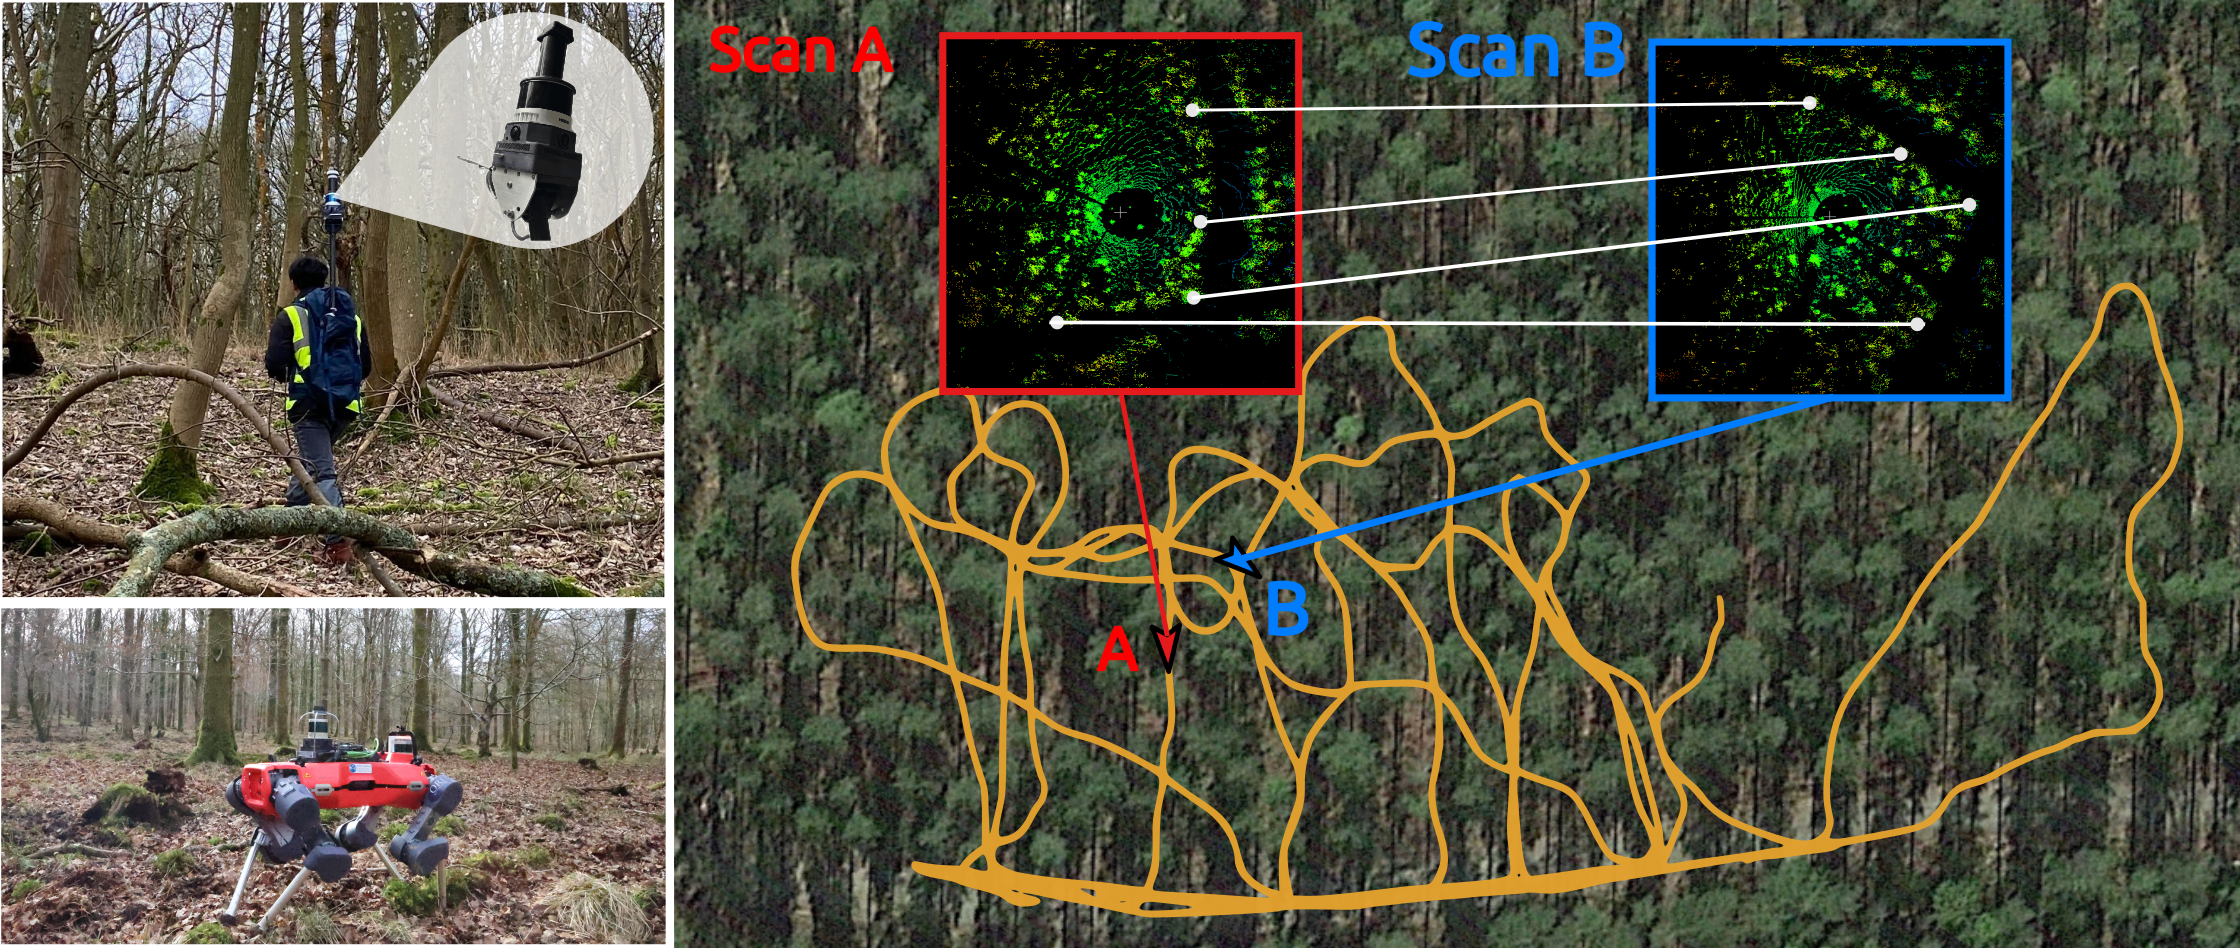
\includegraphics[width=\linewidth]{pics/header.png}
    \captionof{figure}{Place recognition in dense forest environments using a backpack-mounted LiDAR and legged robot equipped with LiDAR. Right: Illustration of loop closure detection within a deeply forested area, with offset distance of 9.2 meters and orientation of 56 degrees between the matched scans. White lines indicate some corresponding locations in the two point clouds (but no actual corresponces are used).
    }
    \label{fig:motivation}
\end{figure}

\subsection*{Motivation}
Place recognition is an essential capability used to minimize the drift in the pose estimate produce by a Simultaneous Localization and Mapping (SLAM), as well as to re-localize in previously mapped areas. 
LiDAR-based place recognition systems have demonstrated robustness by effectively capturing scene structure while showing low susceptibility to visual changes, making them suitable for long-term navigation. 
Previous methods have primarily focused on the problem of autonomous driving in urban environments (characterised by long linear sequences), with their efficacy in natural settings much less tested.
%\mfallon{Wildplaces dataset is a counter example of this.} 
Recent ongoing applications in natural environments, including agriculture, environmental monitoring, conservation, and search and rescue, highlight the significance of extending research efforts beyond urban landscapes.

\subsection*{Challenges in natural environments}
% Why natural environment 
Despite the advancements of LiDAR-based place recognition in urban areas, its application in unstructured natural environments like forests presents several notable challenges. 
Firstly, natural environments are irregular structures like trees, which not only lack fine structure but also undergo seasonal changes, affecting their shape and density over time. This complicates the creation of consistent geometric representations crucial for accurate place recognition.
Secondly, a limited field of view and occlusions of a LiDAR sensor pose a loss of information. In large-scale natural environment, LiDAR sensors often struggle to capture the complete vertical extent of the environment. 
This issue is particularly common in areas with tall, cluttered trees.  Undulating terrains and dense trees cause occlusions resulting in incomplete scans of a LiDAR sensor. 
Lastly, unique, undefined trajectories or paths when exploring dense forests pose another challenge: a place recognition capability of identifying its location not exctly at the same visited place but 'near by' location. 


%%%%%%%%%%%%%%%%%%%
%% WHICH PROBLEM
% Second, explain WHICH problem you are solving/address to solve: Compare WildPlace  
\subsection*{Objectives}
Recently, the Wild-Places dataset \cite{knights2023icra} has been made available. In it a large-scale forest dataset was captured by hand-held spinning LiDAR, capturing seasonal changes within the forest. The dataset was used to evaluate different stete-of-the-art place recognition models in forest environments focusing on localization tasks along the access roads of a national park. The main outcome of their work was that learning-based descriptors such as Logg3dNet \cite{vidanapathirana2022icra} showed better performance compared to handcrafted methods such as ScanContext \cite{kim2018iros}. While the findings suggested that LiDAR-based methods could provide a solution for place-based localization in forest environments, it was not conclusive if the results transferred to dense forest areas, without the strong structural cues that access roads provide roads. Additionally we are also interested in testing the accuracy of precise 6DoF pose estimation for forestry or biodiversity monitoring applications.


%%%%%%%%%%%%%%%%%%%
%% HOW & WHAT
% Third, explain briefly how one can address the problem in general and mention 
% briefly what others/we before have done. Prepare the reader for your contribution that comes in the next section (and not here!).
%\mfallon{this paragraph should be a little literature review - NOT about what we did}
%\haedam{I changed the paragraph to be more about WildPlace}

% In this paper, we extend the evaluation of place recognition models to dense forest environments, employing various setups of LiDAR sensors. For instance, we consider scenarios involving legged robots or backpack-mounted LiDAR devices, which explore the forest in a more unstructured manner, without relying on defined access roads for detecting loop-closures.
% This extension enables for efficient forest mapping and surveying applications in scenarios including single-session and multi-session SLAM, as well as relocalization within a pre-existing map.

%%%%%%%%%%%%%%%%%%%
%% MAIN CONTRIBUTION & WHAT FOLLOWS FROM THAT
% Explain your contribution in one paragraph. This is a very important paragraph. 
% Always start that paragraph with: ``The main contribution of this paper is''
\subsection*{Contributions}

In this work, we present an evaluation of place recognition models to dense forest environments. We employ different LiDAR sensors with sequences recorded with backpack-mounted devices or mobile robots, such as legged platforms, to perform a rigorous analysis of existing learning-based and handcrafted LiDAR place recognition systems. Further, we present a LiDAR-based SLAM system to assess the proposed loop-closure pairs and subsequently validate them through fine-registration in both online and offline modes. Finally, we demonstrate the approach being use for a purely relocalization task, wherein the system continuously localizes its position within a prior point cloud map made up of individual LiDAR scans.

% \mfallon{Note: alternatively you could simply localise in a single giant point cloud of the forest - if you knew the starting point - but that would not scale well. But it would work!}

%%%%%%%%%%%%%%%%%%%
%% OUR KEY CLAIMS (can be merged with the main contribution above if desired)
% Explicitly(!) state your claims in one (short) paragraph and make
% sure you pick them up again in the experiments and support every claim.

In summary, the contributions of this thesis are:
\begin{itemize}

\item Evaluation of the performance of four LiDAR place recognition models, both handcrafted and learning-based, in dense forest environments.

\item Analyzis of loop-closure performance as a function of the relative distance and orientation between candidate loop pairs.

\item Demonstration of the best performing method in online/single-session and offline/multi-session SLAM modes, as well as in relocalization tasks for forest inspection in a prior environment map. 

\item Release of our dense forest datasets with ground truth, collected with a backpack-mounted LiDAR across three different countries\footnote{Our datasets will be published at \url{https://ori.ox.ac.uk/labs/drs/datasets-drs/}} 
\end{itemize}






% \section{Motivation}

% Legged robots have the potential to perform tasks that are extremely challenging or risky for humans, such as exploration of unknown locations or rescue operations. The recent \gls{darpa} SubT challenge (2018-2021) was a clear demonstration of the advantages of such platforms for exploration in urban and underground environments~\cite{Ackerman2022}. When the challenge started in 2018, 3 out of 11 teams were using legged robots for the competition; 3 years later almost every team relied on them as their core platforms~\cite{Chung2023}. Their versatility when negotiating different kinds of terrain compared to wheeled robots, as well as their increased payload capabilities compared to aerial ones offer a good balance for their deployment in the field.

% A key aspect of this success has been the impressive mobility skills achieved by the locomotion controllers developed by the research community over the last few years~\cite{Gangapurwala2020, Miki2022a, Kumar2021}, combined with the consolidation of commercial platforms such as the Boston Dynamics' Spot~\cite{BostonDynamics} and ANYbotics' ANYmal~\cite{Anybotics} quadrupeds, and humanoids such as the Agility Robotics' Digit~\cite{AgilityRobotics}. This offers an unprecedented scenario for their mass adoption in applications such as last-mile delivery, industrial inspection, monitoring, or rescue.

% The new locomotion controllers have unlocked new environments where legged robots can operate: not only warehouses with flat terrain but also industrial environments with complex staircases~\cite{BostonDynamics}, urban and disaster scenarios~\cite{Lee2020}, underground environments~\cite{Miki2022a}, as well as natural scenes such as foThe main objectives are to evaluate the performance of existing LiDAR-based place recognition models in dense forest environments.motivation/motivation.jpg}
% 	\caption{Autonomous deployments of legged robots using the contributions presented in this thesis. They include industrial environments, underground mines, public parks, and forests.}
% 	\label{fig:motivation}
% \end{figure}

% \section{Objective}
% The main objective of this thesis is to develop new navigation systems for legged robots. We define navigation as the problem of safely moving between two locations A and B while avoiding obstacles and other risky areas~\cite{Corke2011,Lynch2017,Ekstrom2018}. While the definition is concise, developing such capabilities for robotic systems is a complex problem that requires a strong coordination of perception, planning, and control methods.

% The second objective is then to develop the specific systems and methods that, when seamlessly integrated, enable legged robot navigation.

% Last, we aim to achieve navigation in challenging environments: spaces that can be dynamic, difficult to access by humans, or simply risky. Specific examples include  industrial facilities, mines, tunnels, or open natural scenes.

% %In this work we present three solutions for this purpose. They address localisation, scene understanding and local planning with legged platforms. These have been tested onboard, in closed-loop, demonstrating real-world navigation in environments such as structured industrial facilities, underground mines, and forests, .

% \section{Contributions}
% The main contribution of this thesis is the investigation, implementation, and field deployment of new navigation systems to expand the use of legged robots in challenging environments, as shown in \figref{fig:motivation}. The systems were designed to be simple but principled, exploiting fundamental ideas of optimisation methods as well as the constraints and advantages that legged robots present.

% The specific contributions of this work include:
% \begin{itemize}[leftmargin=*]
% 	\item An entropy-based approach for active camera selection that robustifies multi-camera localisation systems under transient scene changes.
% 	\item A local planning system that relies on local scene representations to achieve safe and reactive navigation.
% 	\item A framework for self-supervised online traversability learning that enables fast deployment in unknown environments.
% 	\item A mission planning system for autonomous forest inventory with legged robots.
% 	\item Hardware integration and deployment of these systems on legged platforms in industrial, underground, and natural environments.
% \end{itemize}



% \section{Thesis Outline}
% This thesis is presented in the \emph{integrated format} of the University of Oxford. Chapters 4-6 consist of peer-reviewed publications, each one accompanied by additional discussion as well as a Statement of Authorship declaring the author's contribution to each work. Chapter 7 is an original chapter describing a real-world application.

% The remainder of the thesis is structured as follows:
% \begin{itemize}[leftmargin=*]
% 	%\item \textbf{Chapter 1 -- Introduction:} The present chapter, summarising the objectives, contributions, and achievements.
% 	\item \textbf{Chapter 2 -- Background:} Presentation of the main definitions, theory, and methods used in the thesis.
% 	\item \textbf{Chapter 3 - Related Work:} Review of the relevant literature on robot navigation, with a particular focus on legged platforms.
% 	\item \textbf{Chapter 4 -- Multi-camera Visual Localisation:} An approach to reliably localising robots by actively choosing the \emph{most informative} camera during deployment.
% 	\item \textbf{Chapter 5 -- Reactive Local Planning:} How to navigate in challenging, narrow environments using a reactive local planning approach.
% 	\item \textbf{Chapter 6 -- Online Traversability Learning:} Overcoming the challenges of data collection and curation in traversability estimation via online self-supervised learning.
% 	\item \textbf{Chapter 7 -- Autonomous Forest Inventory:} Conceptualisation and field deployment of autonomous legged robots for forestry applications.
% 	\item \textbf{Chapter 8 -- Conclusion:} Discussion on the achievements and limitations of this work, lessons learned, and future directions for the field.
% \end{itemize}
% \chapter{Background}
\label{chap:background}

% This chapter introduces the main concepts and methods used in the remainder of this thesis. I begin by presenting basic notation and mathematical definitions in \secref{sec:preliminaries}. Then I present the core ideas of least squares optimisation in \secref{sec:optimisation}, as it is the core machinery used for the systems developed in this work. \secref{sec:platforms-sensors} introduces the main sensors used in this work, providing further discussion on camera modelling. I close this chapter with \secref{sec:algorithms-navigation} introducing algorithms for robot navigation, which will be further discussed in the Literature Review (\chapref{chap:lit-review}).

% % =============================================================================
% \section{Preliminaries}
% \label{sec:preliminaries}

% \subsection{Notation}
% To refer to different mathematical objects, such as vectors, matrices or reference frames, we will use different typography styles. The conventions adopted in this thesis are summarised in \tabref{tab:notation}.

% \begin{table}[h]
% 	\centering
% 	\caption{Notation used for mathematical objects.}
% 	\begin{tabular}{lll}
% 		\toprule
% 		\textbf{Quantity} & \textbf{Description}   & \textbf{Example}                         \\
% 		\midrule
% 		Scalars           & Upper/Lowercase italic & The traversability score $s$             \\
% 		Vectors           & Lowercase bold         & The 3D point $\mathbf{p}$                \\
% 		Matrices          & Uppercase bold         & The rotation matrix $\mathbf{R}$         \\
% 		Sets/Manifolds    & Uppercase calligraphic & The map points $\mathcal{P}$             \\
% 		Reference Frames  & Uppercase typewriter   & The \emph{map} frame $\M{}$            \\
% 		                  & (legacy expression)    & The \emph{world} frame $\legacyframe{W}$ \\
% 		\bottomrule
% 	\end{tabular}
% 	\label{tab:notation}
% \end{table}

% \subsection{Rotations and Poses}
% Rotation and rigid-body matrices are particularly important in robotics, as they are widely used to describe how objects are placed and moved in space. In this thesis we adopt the formalisation of \emph{Lie groups} to represent them.

% In brief, Lie groups are defined as both a \emph{group} and a \emph{differentiable manifold}. By being a group: (1) they define a binary operation, (2) the operation is associative, (3) there is an identity element, and (4) each element has an inverse. 
% For example, for rotation and rigid-body matrices (1) is defined by matrix multiplication, which also satifies (2). For (3) they have the identity matrix $\identity$, and (4) is the matrix inverse.

% Their differentiable manifold side reflects the smooth geometric constraints that define a valid member of the group. For example, a 3D orientation has 3 \gls{dof} and it can be represented by a 3D vector using Euler angles or an axis-angle representation~\cite{Barfoot2017}. However, not all vectors in $\R{3}$ are valid orientations, and the constraints that define a valid Euler angle are not encoded in the representation. In contrast, a rotation matrix is an over-parametrised representation ($9$ entries) but with orthonormality constraints; this allows them to effectively represent the intrinsic $3$ \gls{dof} of a valid orientation in a smooth manner---which defines the manifold.

% This section provides basic definitions used across the manuscript; additional machinery is further explained in the specific chapters when required. For an in-depth, technical presentation refer to \textcite{Sola2018} or \textcite{Calinon2020}; for a practical overview, see my tutorial~\cite{Mattamala2021b}.

% \subsubsection{Rotation Matrices}
% Rotation matrices are formally part of the \emph{Special Orthogonal Group} or $\SOn{}$. It is the set of all matrices $\rotation{}{}$ that satisfy orthonormality $\rotation{}{}^{\top}\rotation{}{} = \identity$, as well as $\det{\rotation{}{}} = 1$.

% In this thesis we are interested in the space of 2D rotations on the plane $\SOtwo$, as well as the space of 3D rotations $\SOthree{}$.

% \subsubsection{Rigid-body Matrices}
% The group of rigid-body matrices is known as \emph{Special Euclidean Group} or $\SEn$. They represent a relative 6 \gls{dof} transformation or \emph{pose}, i.e. traslation and rotation. Their matrix structure is given by:
% \begin{equation}
% 	\pose{}{} = \matrixSE{ \rotation{}{} }{ \nvec{t} }
% \end{equation}

% In this thesis we are concerned specifically about the group of planar transformations $\SEtwo$, where $\rotation{}{} \in \SOtwo$ and $\nvec{t} \in \R{2}$, as well as the group of 3D transformations $\SEthree$, where $\rotation{}{} \in \SOthree$ and $\nvec{t} \in \R{3}$.

% \subsection{Frames}
% The mathematical quantities we will use are not abstract concepts but they are associated to the physical world. Concretely, they are represented with respect to \emph{reference frames} that define a \emph{point-of-view} used to describe them. This is particularly important not only for modelling~\cite{Furgale2014} but also the definitions used in software tools widely used in robotics such as the \gls{ros}~\cite{Meeussen2010}. The main reference frames we use in this work are shown in \tabref{tab:frames}.
% \begin{table}[h]
% 	\centering
% 	\caption{Main reference frames used in this work.}
% 	\begin{tabular}{cl}
% 		\toprule
% 		\textbf{Frame} & \textbf{Description}                                                         \\
% 		\midrule
% 		$\B$           & \emph{base} or \emph{body} frame specified at the center of the robot's body \\
% 		$\I$           & \emph{odometry} or \emph{inertial} fixed frame used by odometry estimators   \\
% 		$\M$           & \emph{map} fixed frame to specify the origin of the robot's map              \\
% 		$\Sensor$      & \emph{sensor} frame usually defined with respect to the base frame           \\
% 		\bottomrule
% 	\end{tabular}
% 	\label{tab:frames}
% \end{table}

% We can then endow the aforementioned mathematical notation with special subindices to specify their relationship with the relevant frames. This is graphically illustrated in \figref{fig:frames}.

% \begin{figure}[t]
% 	\centering
% 	\includegraphics{figures/inkscape/frames}
% 	\caption[short version]{Main reference frames and frame-endowed notation used in this thesis. We adopt the axes colour convention with the \textcolor{CustomRed}{x-axis in \textbf{red}}, \textcolor{CustomGreen}{y-axis in \textbf{green}}, and \textcolor{CustomBlue}{z-axis in \textbf{blue}}. The inertial frame $\I$ and the map frame $\M$ are fixed, the base frame $\B$ moves with the robot, while the sensor frame $\Sensor$ is fixed relative to $\B$ through the rigid-body transformation $\pose{\M}{\B}$. The linear velocity of the base is given by the vector $\point{v}{\B}$. The fixed 3D point in the frame $\I$ is denoted by $\point{p}{\I}$.}
% 	\label{fig:frames}
% \end{figure}

% % =============================================================================
% \section{Optimisation}
% \label{sec:optimisation}
% Optimisation is at the core of many robotics problems. In particular, squared cost minimisation problems, known as \gls{ls}, are one of the most commonly used formulations to solve state estimation, motion planning, and learning~\cite{Dellaert2017,Bishop2006}. We review the basic concepts and methods that will be used in the following chapters of the thesis.

% \subsection{Linear Least Squares}
% We begin with the simplest \gls{ls} formulation. Let us consider a linear model:
% \begin{equation}
% 	f(\nvec{x}) = \nmat{A}\nvec{x} + \nvec{b}
% \end{equation}
% with $\nvec{x} \in \R{n}$ an unknown variable, and $\nvec{b} \in \R{m}$, and $\nmat{A} \in \R{m\times n}$ hyper-parameters of the model.

% We would like to estimate the value of the variable $\nvec{x}$, given empirical samples of the linear model $\nvec{y}_{i} \in \R{m}$, with $i=1,\ldots,N$. For some value of $\nvec{x}$, we can characterise how well the linear model approximates each sample $\nvec{y}_{i}$ by means of the \emph{residual function}:
% \begin{equation}
% 	\nvec{r}_{i} (\nvec{x}) =  \nmat{y}_{i} - \left(\nmat{A}_{i}\nvec{x} + \nvec{b}_{i} \right)
% \end{equation}

% Then, the \gls{ls} estimate of $\nvec{x}$, denoted $\nest{\nvec{x}}$, is the estimate that minimises the \emph{cost} or \emph{loss} function $\loss{}\left( \nvec{x}\right)$ defined as the sum of the squared residuals for all the data samples:
% \begin{align}
% 	\nest{\nvec{x}} & = \argmin_{\nvec{x}} \loss{}\left( \nvec{x}\right)                                                                         \\
% 	                & = \argmin_{\nvec{x}} \sum^{N}_{i} \lsq{\nvec{r}_{i} (\nvec{x})}{}                                                          \\
% 	                & = \argmin_{\nvec{x}} \sum^{N}_{i} \lsqexp{\left( \nmat{y}_{i} - \left(\nmat{A}_{i}\nvec{x} + \nvec{b}_{i} \right) \right)}
% \end{align}

% Sometimes not all the data samples have the same importance, and we would like to scale the contribution of the set of samples or specific dimensions. We introduce an additional matrix $\nmat{\Sigma}_{i}$, usually diagonal, as a hyper-parameter to control this:
% \begin{align}
% 	\label{eq:weighted-ls}
% 	\nest{\nvec{x}} & = \argmin_{\nvec{x}} \sum^{N}_{i} \lsq{\nvec{r}_{i} (\nvec{x})}{\nmat{\Sigma}_i}                                                                   \\
% 	                & = \argmin_{\nvec{x}} \sum^{N}_{i} \lsqexpcov{\nvec{r}_{i} (\nvec{x}) }{\nmat{\Sigma}_{i}}                                                          \\
% 	                & = \argmin_{\nvec{x}} \sum^{N}_{i} \lsqexpcov{\left( \nmat{y}_{i} - \left(\nmat{A}_{i} \nvec{x} + \nvec{b}_{i} \right) \right) }{\nmat{\Sigma}_{i}}
% \end{align}
% which corresponds to the most general version of linear \gls{ls} we will consider in the rest of the manuscript.

% \subsubsection{Solving the Problem}
% To solve \eqref{eq:weighted-ls}, it is necessary to linearise the quadratic cost. As the problem is convex, the linearisation produces a set of linear equations for each residual known as \emph{normal equations}:
% \begin{align}
% 	\nmat{A}_{1}^{\top}\, \nmat{\Sigma}_{1}^{-1}\, \nmat{A}_{1}\, \nest{\nvec{x}} & = \nmat{A}_{1}^{\top}\, \nmat{\Sigma}_{1}^{-1}\, \nvec{b}_{1} \\
% 	\cdots                                                                        &                                                               \\
% 	\nmat{A}_{N}^{\top}\, \nmat{\Sigma}_{N}^{-1}\, \nmat{A}_{N}\, \nest{\nvec{x}} & = \nmat{A}_{N}^{\top}\, \nmat{\Sigma}_{N}^{-1}\, \nvec{b}_{N}
% \end{align}

% which can be rearranged and stacked together as a single linear system:
% \begin{equation}
% 	\label{eq:normal-equations}
% 	\left( \nmat{A}^{\top}\, \nmat{\Sigma}^{-1}\, \nmat{A}\, \right) \nest{\nvec{x}} = \nmat{A}^{\top}\, \nmat{\Sigma}^{-1}\, \nvec{b}
% \end{equation}

% The matrix on the left-hand side is known as the \emph{Hessian}:
% \begin{equation}
% 	\label{eq:hessian}
% 	\nmat{A}^{\top} \nmat{\Sigma}^{-1} \nmat{A}
% \end{equation}

% By inverting the Hessian, we can recover the estimate of $\nest{\nvec{x}}$ in closed-form:
% \begin{equation}
% 	\nest{\nvec{x}} = \left( \nmat{A}^{\top} \nmat{\Sigma}^{-1} \nmat{A} \right)^{-1} \nmat{A}^{\top} \nmat{\Sigma}^{-1} \nvec{b}
% \end{equation}

% While this process is straightforward, it can be expensive to compute when the dimensionality of $\nvec{x}$ is large. Standard procedures to solve \gls{ls} include factorising the Hessian in the normal equations (\eqref{eq:normal-equations}) using Cholesky or QR factorisarion~\cite{Golub2013}.

% Exploiting the structure of the Hessian matrix with problem-specific knowledge has also been heavily exploited in robotics to achieve real-time performance. Some examples are Square Root SAM~\cite{Dellaert2006} and \gls{isam}~\cite{Kaess2008} for incremental state estimation, or KOMO for receding-horizon motion planning~\cite{Toussaint2017}.

% \subsubsection{Probabilistic Interpretation}
% The formulation of \gls{ls} used in \eqref{eq:weighted-ls} has a probabilistic interpretation: It is the \gls{map} formulation of an estimation problem with random variables that follow a Gaussian distribution. In particular, if we consider the residual to follow a zero-mean Gaussian distribution with covariance $\nmat{\Sigma}_{i}$:
% \begin{equation}
% 	\label{eq:gaussian-factor}
% 	\nvec{r}_{i} (\nvec{x}) \sim \gaussian{\nvec{0}}{\nmat{\Sigma}_{i}}
% \end{equation}

% Then the \gls{map} is given by:
% \begin{equation}
% 	\label{eq:map}
% 	\nest{\nvec{x}} = \argmax_{\nvec{x}} \prod_{i}^{N} { \fullgaussian{ -\frac{1}{2} \lsqexpcov{ \nvec{r}_{i} (\nvec{x}) }{\nmat{\Sigma}_{i} } }{ \nmat{\Sigma}_{i} }{m} }
% \end{equation}

% To show that it is equivalent to \gls{ls}, we simply compute the negative logarithm of \eqref{eq:map}:
% \begin{equation}
% 	\label{eq:map-sq}
% 	\nest{\nvec{x}} = \argmin_{\nvec{x}} \sum^{N}_{i} \frac{1}{2} \lsqexpcov{\nvec{r}_{i} (\nvec{x}) }{\nmat{\Sigma}_{i}} + \ln{\left( \gaussiannorm{\nmat{\Sigma}_{i}}{m} \right)}
% \end{equation}
% As we are only interested in the terms that depend on $\nvec{x}$, we can disregard the term on the right, as well as the scaling $\frac{1}{2}$. This optimisation is then equivalent to \eqref{eq:weighted-ls}.

% Additionally, we can rewrite \eqref{eq:map} as:
% \begin{equation}
% 	\label{eq:factors}
% 	\nest{\nvec{x}} = \argmax_{\nvec{x}} \prod_{i}^{N} { \phi(\nvec{x}) }
% \end{equation}
% Which expresses the problem as a product of factors. This has an equivalent representation in the graphical models literature, known as a \emph{factor graph}~\cite{Dellaert2017}. Hence, for the particular case of Gaussian factor graphs, where factors are defined by \eqref{eq:gaussian-factor}, solving an inference problem on the factor graph is equivalent to \gls{ls}.


% \subsubsection{Interpretations of the Hessian}
% The Hessian (\eqref{eq:hessian}) has important interpretations. Geometrically, the Hessian is the second derivative of the \gls{ls} cost function. Hence, it represents the curvature around the minimum. If we consider the cost function as a manifold, then the Hessian also defines the \emph{Riemannian metric} of the manifold~\cite{Toussaint2017}---this idea will be important for the local planner presented in \chapref{chap:local-planning}. Probabilistically, it is the \emph{Fisher Information Matrix} $\nmat{I}_{\mathrm{Fisher}}$. Its inverse corresponds to the covariance matrix of the \gls{map} estimate $\nmat{I}_{\mathrm{Fisher}}^{-1} = \nest{\nmat{\Sigma}}$. When the posterior of the \gls{map} is fitted with $\gaussian{ \nest{\nvec{x}} }{\nest{\nmat{\Sigma}}}$, the approximation is known as \emph{Laplace approximation}~\cite{Bishop2006}.

% The probabilistic interpretation allows us to study the \gls{ls} solution further. For example, under the Gaussian approximation we can determine the \emph{entropy} $H$ of the estimate, which represents its quality. It is defined as:
% \begin{equation}
% 	H\left(\nest{\nvec{x}} \right) = \frac{1}{2}n \left(1 + \ln{(2\pi)}) \right) + \frac{1}{2} \ln{\left( \det{\nest{\nmat{\Sigma}}} \right)}
% \end{equation}

% We can use the entropy to compare the quality different \gls{ls} estimates. However, we observe that (1) it only depends on $\nest{\nmat{\Sigma}}$, so we can ignore the constant terms, (2) we require to invert $\nmat{I}_{\mathrm{Fisher}}$ to obtain $\nest{\nmat{\Sigma}}$. Hence, we can use the \emph{negative entropy} as proposed by \textcite{Kuo2020}:
% \begin{equation}
% 	E\left( {\nest{\nvec{x}}} \right) = \ln{\left( \det{ \nmat{I}_{\mathrm{Fisher}} } \right)} = \ln{\left( \det{ \left( \nmat{A}^{\top} \nmat{\Sigma}^{-1} \nmat{A} \right) } \right) }
% \end{equation}
% This is a positive scalar value that will be used in \chapref{chap:visual-localisation} to compare different estimates obtained from \gls{ls}.

% \subsection{Non-linear Least Squares}
% The previous formulation of \gls{ls} is useful to understand the basic principles but it is not the one usually found in real robotics problems. A more general approach is minimise a cost $\loss{}\left( \nvec{x}\right)$ with squared non-linear residuals, known as \gls{nls}:
% \begin{align}
% 	\label{eq:weighted-nls}
% 	\nest{\nvec{x}} & = \argmin_{\nvec{x}} \sum^{N}_{i} \lsq{\nvec{r}_{i} (\nvec{x})}{\nmat{\Sigma}_i}     \\
% 	                & = \argmin_{\nvec{x}} \sum^{N}_{i} \lsq{ f(\nvec{x}, \nvec{y}_{i}) }{\nmat{\Sigma}_i}
% \end{align}
% with $f$ a non-linear function of the variables $\nvec{x}$ and the data $\nvec{y}_{i}$.

% \subsubsection{Solving the Problem}
% To solve \gls{nls}, the most standard procedure is linearising the residuals in \eqref{eq:weighted-nls} with respect to an operation point $\nlin{\nvec{x}}$:
% \begin{equation}
% 	\label{eq:linearisation}
% 	\nvec{r}_{i} (\nvec{x}) \approx \nvec{r}_{i} (\nlin{\nvec{x}} + \delta\nvec{x}) \approx \nvec{r}_{i} (\nlin{\nvec{x}}) + \jac{\nvec{r}_{i}} \left( \nlin{\nvec{x}} \right) \delta\nvec{x}
% \end{equation}
% where $\jac{\nvec{r}_{i}}$ is the \emph{Jacobian} of the residual function with respect to $\nvec{x}$.
% Then, \eqref{eq:weighted-nls} becomes a \gls{ls} problem on the increment $\delta\nvec{x}$ that we can solve in closed-form:
% \begin{align}
% 	\label{eq:linearised-nls}
% 	\delta\nest{\nvec{x}} & = \argmin_{\delta\nvec{x}} \sum^{N}_{i} \lsq{ \nvec{r}_{i} (\nlin{\nvec{x}}) + \jac{\nvec{r}_{i}} \left( \nlin{\nvec{x}} \right) \delta\nvec{x} }{\nmat{\Sigma}_{i}} \\
% 	                      & = \left( \jac{}^{\top} \nmat{\Sigma}^{-1} \jac{} \right)^{-1} \jac{}^{\top} \nmat{\Sigma}^{-1} \nlin{\nvec{x}}
% \end{align}
% with $\jac{}$ a matrix built by stacking the Jacobians of all the residuals $\jac{\nvec{r}_{i}}$.
% The increment $\delta\nest{\nvec{x}}$ is used to update the current estimate of $\nvec{x}$ by using the rule:
% \begin{equation}
% 	\label{eq:update-rule}
% 	\nvec{x} \leftarrow \nlin{\nvec{x}} + \delta\nest{\nvec{x}}
% \end{equation}

% This is the basis of the \gls{gn} algorithm. It solves the \gls{nls} problem by starting from an initial estimate, linearising the cost around it (\eqref{eq:linearisation}), solving the normal equations (\eqref{eq:linearised-nls}), and iteratively updating the estimate (\eqref{eq:update-rule}) until convergence.

% \subsubsection{Alternative Optimisation Approaches}
% Although \gls{gn} provides an straightforward framework to solve \gls{nls}, it has some drawbacks, as computing and inverting the Hessian can be expensive. This is particularly the case when the nonlinear function $f$ is parametrised by a neural network. An alternative approach is defining a simpler rule based on the gradient of the cost function $\grad{\loss{}\left( \nvec{x}\right)}$, known as \emph{gradient descent}:
% \begin{equation}
% 	\label{eq:gradient-descent-rule}
% 	\nvec{x} \leftarrow \nlin{\nvec{x}} - \gamma \grad{\loss{}} \left( \nlin{\nvec{x}} \right)
% \end{equation}

% Where $\gamma$ is known as \emph{step size} or \emph{learning rate}.
% In practice, due to the non-convexity of neural networks, \gls{gd} will not lead to the steepest descent direction. Instead, we can sample random data batches of size $B$ to evaluate the gradient for each sample $i$, $\grad{\loss{i}}\left( \nvec{x}\right)$. Then, we can use the average gradient for the update rule, which is known as \gls{sgd}:
% \begin{equation}
% 	\label{eq:sgd-rule}
% 	\nvec{x} \leftarrow \nlin{\nvec{x}} -  \frac{\gamma}{B} \sum_{i}^{B}{\grad{\loss{i}}\left( \nlin{\nvec{x}} \right)}
% \end{equation}

% Nowadays more sophisticated optimisation methods exists, such as Adam~\cite{Kingma2015}, which are based on \gls{sgd}. Adam is later used to solve an online learning problem in \chapref{chap:traversability-learning}.

% \subsubsection{On the Interpretations of \gls{nls}}
% As a last remark, the same geometric and probabilistic interpretations of \gls{ls} hold for \gls{nls} but only for the current linearisation point. Further, as the optimisation is non-convex, the estimates of the mean and covariance from the Laplace approximation do not hold globally, and they can under or over estimate the covariance of the estimate~\cite[109]{Barfoot2017}.

% % =============================================================================
% \section{Platforms and Sensors}
% \label{sec:platforms-sensors}
% In this section we review the main sensors and platforms used in this work. We first discuss \emph{exteroceptive} sensors, which measure the environment external to the robot. We focus on visual sensors, i.e. cameras, as they are the main sensor used in this thesis. \gls{lidar} sensing is also discussed as it is used in later chapters. \emph{Proprioceptive} sensing, which provides information about the robot's internal state, is just briefly presented.

% We then provide a general overview about legged robots, their distinctive features, and how they differ from other platforms such as wheeled and aerial. This will prepare us for the last section of this chapter, that discusses robot navigation systems.

% \subsection{Cameras}
% Cameras are ubiquitous sensors: they are low-cost, provide rich appearance information about the external world, and operate at reasonable frequency (\SIrange{10}{30}{\hertz}) given the typical speed of the majority of robotics platforms. When combined with other cameras (stereo systems) or active lighting (e.g. structured light), they can also measure 3D information. The main cameras used in this thesis are the Intel Realsense camera, and the Sevensense Core Research multi-camera unit, shown in \figref{fig:cameras}.

% \begin{figure}[t]
% 	\centering
% 	\includegraphics[height=3cm,clip,trim={0cm -0.2cm 0cm -0.2cm}]{figures/cameras/realsense.png}
% 	\hspace{1cm}
% 	\includegraphics[height=2.7cm,clip,trim={0cm -0.2cm 0cm -0.2cm}]{figures/cameras/alphasense.png}
% 	\caption{Main camera units used in this work. \textbf{Left:} Intel \emph{Realsense D435i} stereo and depth visual-inertial unit. Source: Intel. \textbf{Right:} Sevensense \emph{Core Research} multi-camera visual-inertial sensor (formerly \emph{Alphasense Core}). Source: Sevensense.}
% 	\label{fig:cameras}
% \end{figure}

% Their basic operating principle is based on a regular array of light-sensitive \emph{pixels}, known as \emph{digital image sensor}. Each pixel outputs a signal that is proportional to the number of photons received in a fixed \emph{exposure time}, which also determines the maximum operating frequency (\SIrange{10}{30}{\hertz}). Colour cameras additionally have colour filters for each pixel (red, green, blue); their arrangement is known as \emph{Bayer pattern}.

% Producing a visually appealing image from the pixels' signals and the Bayer pattern requires low-level processing provided by a \gls{isp}. The \gls{isp} is usually implemented on dedicated hardware, and it performs different operations that include demosaicing, gamma correction, white balance, and tone mapping~\cite{Delbracio2021}. While this is usually provided by manufacturers for commercial cameras, this is not necessarily the case for experimental kits such as the Alphasense.

% As part this thesis, a \gls{ros}-compatible \gls{isp} for the Alphasense was developed, which performs debayering, white balancing, and lens undistortion, among other steps. The package is open-source and available as \texttt{raw\_image\_pipeline}\footnote{\url{https://github.com/leggedrobotics/raw_image_pipeline}}.

% Once monochromatic (greyscale) or colour (RGB) images are produced, we can perform further processing~\cite{Corke2011}. As we are interested in obtaining 3D information from the world, we need to model the geometry of the image projection process. This is explained in the following sections.

% \subsubsection{Camera Projection Geometry}
% We begin by modelling the geometry of the projection process, as it has a primary role in \chapref{chap:visual-localisation} and \chapref{chap:traversability-learning}.

% We consider that the camera has a pose $\pose{\M}{\C} \in \SEthree$ in a fixed frame $\M$. In computer vision textbooks~\cite{Szeliski2022,Hartley2004,Ma2004}, this matrix is known as the \emph{camera extrinsics}. In robotics we usually estimate the pose of the robot body's instead of the sensor's, so we define the extrinsics as the product $\pose{\M}{\C} = \pose{\M}{\B} \pose{\B}{\C}$, where $\pose{\M}{\B}$ is the \emph{robot's body pose}, and $\pose{\B}{\C}$ is the \emph{extrinsic calibration matrix of the camera with respect to the robot's body}, which is obtained from prior calibration.

% Then, a 3D point in homogeneous coordinates $\point{p}{\M} = \left[ X, Y, Z, 1 \right] \in \R{4}$ in the map frame $\M$ is related to the point $\point{p}{\Sensor}$ in sensor frame $\Sensor$ by the projection model $\mathbf{\pi}\left(\point{p}{\Sensor}, \point{p}{\M}\right)$, which is illustrated in \figref{fig:pinhole-model}. The specific steps to achieve this are explained as follows.

% \begin{figure}[h]
% 	\centering
% 	\includegraphics[width=\textwidth]{figures/inkscape/pinhole.pdf}
% 	\caption{The pinhole camera model $\mathbf{\pi}\left(\point{p}{\Sensor}, \point{p}{\M}\right)$ projects the 3D point $\point{p}{\M}$ in the map frame, to the image cordinates $\point{p}{\Sensor}$, given the extrinsic matrix $\pose{\M}{\C}$.}
% 	\label{fig:pinhole-model}
% \end{figure}

% \paragraph{Step 1: Represent the Point in the Camera Frame}
% We first change the reference frame of $\point{p}{\M}$ from $\M$ to the \emph{camera} frame $\C$ (also called \emph{optical frame}):
% \begin{equation}
% 	\label{eq:pinhole-extrinsics}
% 	\point{p}{\C} = \pose{\M}{\C}^{-1}\, \point{p}{\M}
% \end{equation}
% The resulting point $\point{p}{\C}$ is also in homogeneous coordinates but now with respect to the frame $\C$.

% \paragraph{Step 2: Pinhole Projection}
% We then apply the \emph{pinhole projection model}:
% \begin{equation}
% 	\label{eq:pinhole-proj}
% 	\point{p}{\Sensor}' = \Kmat{\Sensor}{\C}\, \point{p}{\C}
% 	%
% 	= \begin{bmatrix}
% 		f_x & 0   & c_x & 0 \\
% 		0   & f_y & c_y & 0 \\
% 		0   & 0   & 1   & 0 \\
% 		0   & 0   & 0   & 1
% 	\end{bmatrix}
% 	\begin{bmatrix}
% 		X\ \\
% 		Y\ \\
% 		Z\ \\
% 		1\
% 	\end{bmatrix}
% 	%
% 	= \begin{bmatrix}
% 		f_x X + c_x Z\ \\
% 		f_y Y + c_y Z\ \\
% 		Z\             \\
% 		1\
% 	\end{bmatrix}
% 	=
% 	\begin{bmatrix}
% 		x \\
% 		y \\
% 		z \\
% 		1
% 	\end{bmatrix}
% \end{equation}

% Where $\Kmat{\Sensor}{\C} \in \R{4\times4}$ is the \emph{intrinsic calibration} matrix. $f_x$ and $f_y$ are the camera focal lengths, while $c_x$ and $c_y$ are the coordinates of the center of the image. They are obtained used standard camera calibration packages, such as Kalibr~\cite{Furgale2013,Rehder2016}.

% \paragraph{Step 3: Normalise the Coordinates}
% The point on the image plane $\I$, denoted $\point{p}{\Sensor}$, is obtained by dividing $\point{p}{\Sensor}'$ by the third component. This produces the normalised image coordinates (\textcite{Szeliski2022}):
% \begin{equation}
% 	\label{eq:pinhole-proj-norm}
% 	\point{p}{\Sensor} = \frac{\point{p}{\Sensor}'}{\point{p}{\Sensor}'_{\left[ 3 \right]}}
% 	=
% 	\frac{1}{z}
% 	\begin{bmatrix}
% 		x \\
% 		y \\
% 		z \\
% 		1
% 	\end{bmatrix}
% 	=
% 	\begin{bmatrix}
% 		x / z \\
% 		y / z \\
% 		1     \\
% 		1 / z
% 	\end{bmatrix}
% 	%
% 	= \begin{bmatrix}
% 		u \\
% 		v \\
% 		1 \\
% 		d
% 	\end{bmatrix}
% \end{equation}

% Here $(u,v)$ denote the pixel coordinates of the projected point on the image plane, and $d$ its \emph{disparity} (inverse depth).

% \subsubsection{Moving Back from Images to 3D}
% An advantage of this formulation, is that in order to \emph{back-project} an image point back into the 3D world, we can easily invert the operations:

% \paragraph{Step 1: De-normalisation} Using the disparity $d$:
% \begin{equation}
% 	\label{eq:pinhole-backproj-norm}
% 	\point{p}{\Sensor}' = \frac{\point{p}{\Sensor}}{\point{p}{\Sensor}_{\left[ 4 \right]}}
% 	=
% 	\frac{1}{d}
% 	\begin{bmatrix}
% 		u \\
% 		v \\
% 		1 \\
% 		d
% 	\end{bmatrix}
% 	=
% 	\begin{bmatrix}
% 		u / d \\
% 		v / d \\
% 		1 / d \\
% 		1
% 	\end{bmatrix}
% \end{equation}

% \paragraph{Step 2: Back-project} Using the inverse of the camera instrinsics matrix:
% \begin{equation}
% 	\label{eq:pinhole-backproj}
% 	\point{p}{\C} = \Kmat{\Sensor}{\C}^{-1}\, \point{p}{\I}'
% 	%
% 	= \begin{bmatrix}
% 		1 / f_x & 0       & -c_x / f_x & 0 \\
% 		0       & 1 / f_y & -c_y / f_y & 0 \\
% 		0       & 0       & 1          & 0 \\
% 		0       & 0       & 0          & 1
% 	\end{bmatrix}
% 	\begin{bmatrix}
% 		u / d\ \\
% 		v / d\ \\
% 		1 / d\ \\
% 		1\
% 	\end{bmatrix}
% 	%
% 	= \begin{bmatrix}
% 		f_x / d \left( u - c_x \right) \ \\
% 		f_y / d \left( v - c_y \right)   \\
% 		1 / d\                           \\
% 		1\
% 	\end{bmatrix}
% \end{equation}

% Please note that this is not possible for all kinds of cameras. Monocular cameras only provide the image coordinates $(u,v)$ and the disparity $d$ is not observable. In this case, the resulting $\point{p}{\C}$ is valid \emph{up to a scale factor} $1/d$. This is also interpreted as monocular cameras being \emph{bearing sensors}: they can only measure a ray (direction) to the true 3D point.

% For stereo cameras, we can estimate the disparity by using the \emph{baseline} $b$ of the camera, which is typically provided by the manufacturer or custom calibration. Given the measurements $(u_l, v_r)$ and $(u_r, v_r)$ from the left and right cameras of a stereo pair, the disparity is determined by:
% \begin{equation}
% 	\label{eq:disparity-stereo}
% 	d = \frac{u_l - u_r}{b}
% \end{equation}

% For depth cameras, the distance to the 3D point, denoted $z$, is measured directly via structured light or \gls{tof} imaging:
% \begin{equation}
% 	\label{eq:disparity:depth}
% 	d = \frac{1}{z}
% \end{equation}

% \paragraph{Step 3: Back to World Frame} Finally we obtain the 3D point in the world frame $\M$ using the extrinsics matrix:
% \begin{equation}
% 	\label{eq:pinhole-backproj-extrinsics}
% 	\point{p}{\M} = \pose{\M}{\C}\, \point{p}{\C}
% \end{equation}

% The aforementioned steps are usually summarised by the \emph{projection function} $\mathbf{\pi}(\cdot)$ and \emph{back-projection function} $\mathbf{\pi}^{-1}(\cdot)$.

% \subsubsection{Applications}
% The pinhole model expresses the fundamental principles that relate images with the 3D structure of the environment. This enables different applications for robotics that are used in the subsequent chapters of this thesis, which are briefly discussed here.

% \paragraph{Visual Localisation} In \chapref{chap:visual-localisation} we will apply the pinhole model for visual localisation using the \gls{pnp}~\cite{Fischler1981} algorithm and factor graph-based pose estimation. These methods minimise the \emph{reprojection error} between a set of image measurements $\point{z}{\Sensor}_{i}$ and the 2D projection of 3D map points $\point{p}{\M}_{i}$, as illustrated in \figref{fig:pinhole-application-localisation} and further discussed in \secref{sec:navigation-state-estimation}.
% \begin{figure}[h]
% 	\centering
% 	\includegraphics{figures/inkscape/visual_localisation.pdf}
% 	\caption{\emph{Visual localisation} methods minimise the reprojection error the idealised projection of 3D points $\point{p}{\M}_{i}$ and image measurements $\point{z}{\Sensor}_{i}$. We use these principles in \chapref{chap:visual-localisation}.}
% 	\label{fig:pinhole-application-localisation}
% \end{figure}

% \paragraph{Elevation Mapping} The principles of camera geometry can be applied to produce dense point clouds using stereo cameras or \gls{tof} imaging, and then generate a local 2.5D elevation map, as shown in \figref{fig:pinhole-application-elevation}. This local representation is used for efficient local planning in \chapref{chap:local-planning}.
% \begin{figure}[h]
% 	\centering
% 	\includegraphics{figures/inkscape/elevation_mapping.pdf}
% 	\caption{\emph{Elevation mapping} relies on the back-projected image points using stereo or depth information to ray-cast them onto a planar grid that encodes the point's height. This grid representation is used for local planning in \chapref{chap:local-planning}. }
% 	\label{fig:pinhole-application-elevation}
% \end{figure}

% \paragraph{Self-supervision} In \chapref{chap:traversability-learning}, we will use the projection model to project the path traversed by the robot by integrating the footprint over time (see \figref{fig:pinhole-application-selfsupervision}). We will use this information as a supervision signal to learn a model to predict which areas are accessible by the robot. 
% \begin{figure}[h]
% 	\centering
% 	\includegraphics{figures/inkscape/self_supervision.pdf}
% 	\caption{By integrating the robot's traversed path over time and projecting it onto past images, we can generate a \emph{supervision signal} used to train models of terrain traversability, as will be shown in \chapref{chap:traversability-learning}}.
% 	\label{fig:pinhole-application-selfsupervision}
% \end{figure}

% \subsubsection{Lens Distortion}
% In the previous applications we did not consider the non-linear effects produced by the camera lenses, which distort how the points are projected on the image plane. Lens distortion models compensate for these effects, so the projections and other operations stay invariant.

% For cameras such as the Realsense (\figref{fig:cameras}, left), these effects can be compensated using a \emph{radial-tangential} model~\cite{Brown1966}. Wide-angle cameras such as the Alphasense unit (\figref{fig:cameras}, right) are modelled by \emph{equidistant} distortion~\cite{Xiong1997} instead. Both models are available in camera calibration packages such as Kalibr~\cite{Furgale2013,Rehder2016}, which enable us to use the same projection principles regardless of the specific camera being used.

% \begin{figure}[t]
% 	\centering
% 	\includegraphics[height=5cm]{figures/cameras/alphasense_color.png}
% 	\hspace{0.4cm}
% 	\includegraphics[height=5cm]{figures/cameras/alphasense_undistorted.png}
% 	\caption{Fisheye lens distortion in the Sevensense Core Research sensor. \textbf{Left:} Distorted output before fisheye correction, henceforth displaying curved trees. \textbf{Right:} Undistorted image, correctly displaying the trees standing straight. The empty pixels (black) represent areas that are not observed in the original input; these are introduced to match the specified intrinsics after undistortion.}
% 	\label{fig:fisheye-distortion}
% \end{figure}

% \subsection{LiDAR}
% \gls{lidar} is another common exteroceptive sensor in robotics, which provides 3D information about the environment. In contrast to (monocular) cameras, they can directly measure distance, achieving centimetre-accurate range measurement up to \SI{100}{\meter}. 

% Distance measurements are obtained by projecting a laser beam into the environment and measuring the time it takes to return. As this process occurs along a single ray, \glspl{lidar} use fixed laser arrays and rotating mirrors to generate 2D or 3D scans. As a result, \glspl{lidar} operate at slightly lower frequencies than cameras, up to \SI{20}{\hertz}. 

% In the remainder of the thesis, \glspl{lidar} are used only as a complementary sensor for evaluation purposes (\chapref{chap:visual-localisation}), or as another complementary source of 3D information (\chapref{chap:local-planning} and \chapref{chap:traversability-learning}). In \chapref{chap:autonomous-forest-inventory} they will acquire a more important role as they provide the main data input for autonomous forest inventory. Some of the devices discussed in this thesis are shown in \figref{fig:lidars}.

% \begin{figure}[t]
% 	\centering
% 	\includegraphics[height=3cm,clip,trim={0cm -0.2cm 0cm -0.2cm}]{figures/lidars/velodyne.png}
% 	\hspace{2cm}
% 	\includegraphics[height=3cm,clip,trim={0cm -0.2cm 0cm -0.2cm}]{figures/lidars/bpearl.png}
% 	\hspace{2cm}
% 	\includegraphics[height=3cm,clip,trim={0cm -0.2cm 0cm -0.2cm}]{figures/lidars/tls.png}
% 	% \caption{Some \gls{lidar} units relevant for the thesis. \textbf{Left:} Velodyne \emph{VLP-16} \SI{360}{\degree} \gls{lidar}. \textbf{Center:} RoboSense \emph{BPearl} \SI{360}{\degree} $\times$ \SI{90}{\degree} unit. \textbf{Right:} Leica \emph{RTC360} \gls{tls} laser scanner.}
% 	\caption{\glspl{lidar} relevant to this thesis. \textbf{Left:} Velodyne \emph{VLP-16} \gls{lidar}. \textbf{Center:} RoboSense \emph{BPearl}. \textbf{Right:} Leica \emph{RTC360} \gls{tls}.}
% 	\label{fig:lidars}
% \end{figure}


% \subsection{Proprioceptive Sensing}
% Proprioceptive sensors provide information about the robot's internal state. The main examples we consider are \glspl{imu} and joint sensors, as they give important context for the navigation algorithms that will be discussed in \secref{sec:algorithms-navigation}, although their are not the main focus of this thesis.

% \emph{\glspl{imu}} provide high-frequency ($>$\SI{100}{\hertz}) angular velocity and linear acceleration measurements. This enables robots to have access to their attitude with respect to gravity, as well as an estimate of the relative translation by time-integration of the measurements~\cite{Woodman2007}. However, they can suffer from thermo-mechanical effects that degrade this estimate, which depends on the \gls{imu} grade, and additional actions need to be taken to compensate for this effects, such as sensor fusion~\cite{Corke2007}.

% \emph{Joint sensors} provide the position, velocity, or torque of a specific joint. As they are usually part of the actuators' hardware for joint-level control, they also operate at higher frequencies ($>$\SI{1}{\kilo\hertz}). In combination with the robot description (e.g. \gls{urdf}), they can provide real-time information about the kinematic configuration of the robot or interacting forces.

% \subsection{Legged Robots}
% Legged robots are a type of mobile robot characterised by the use of limbs to locomote. Among legged platforms, the main distinctive feature is the number of legs used for locomotion. Engineers have developed single-leg hoppers (1 leg), bipeds and humanoids (2 legs), quadrupeds (4 legs), and hexapods (6 legs)~\cite{Kajita2016}.

% In this thesis we focus on quadrupedal platforms. Quadrupeds offer a good balance between robustness, cost, and control complexity compared to other legged robots, as they have the minimal number of legs to statically locomote~\cite{Hutter2013}.

% The main advantage legged robots offer over other ground platforms, such as wheeled robots, is their advanced mobility skills to traverse different types of terrain, including human-made and natural ones. Compared to aerial platforms such as small-size drones, they can carry heavier payloads in longer missions.

% In \tabref{tab:robot-comparison} we compare the main legged platforms commercially available (as of the writing of this manuscript), to other popular platforms such as wheeled robots and drones. This will be relevant in \chapref{chap:autonomous-forest-inventory} to contextualise the use of legged robot in forestry. It also summarises the general characteristics of the ANYbotics ANYmal~\cite{Hutter2017, Anybotics} robot, which is the main platform used for the development of this thesis.

% % Add table
% \begin{table}[h]
% 	\centering
% 	\caption{Specifications of different commercial robotic platforms. ANYmal C is the main robot used in this thesis.}
% 	% \begin{threeparttable}
% \scriptsize
% \renewcommand{\arraystretch}{2}
% %               Robot            & Image          & Type           & Dimensions       & Weight          & Payload         & Max Speed       & Run time        & IP Rating}      & Website}
% \begin{tabular}{m{0.1\textwidth} m{0.1\textwidth} m{0.07\textwidth} m{0.08\textwidth} m{0.07\textwidth} m{0.08\textwidth} m{0.06\textwidth} m{0.05\textwidth} m{0.05\textwidth} m{0.04\textwidth}}
% \toprule
% \textbf{Name}                                & \textbf{Robot}                                                                                                                                           & \textbf{Type} & \textbf{Size (LxWxH)}                                       & \textbf{Weight}        & \textbf{Payload}     & \textbf{Max Speed}                              & \textbf{Run time} & \textbf{IP rat.}   & \textbf{Web}                                                                           \\ \midrule
% \rowcolor{CustomLightGrey}ANYbotics ANYmal C & \begin{minipage}{.09\textwidth}\includegraphics[width=\textwidth, height=\textwidth, keepaspectratio]{figures/robots/anymalc.png}        \end{minipage}  & Legged        & \qtyproduct{1054 x 520 x 830}{\milli\meter}\tnote{$\star$}  & \SI{50}{\kilo\gram}    & \SI{10}{\kilo\gram}  & \SI{1.0}{\meter\per\second}                     & \SI{1.5}{\hour}   & IP67               & --                                                                                     \\ %\hline
% ANYbotics ANYmal D                           & \begin{minipage}{.1\textwidth}\includegraphics[width=0.9\textwidth, height=0.9\textwidth, keepaspectratio]{figures/robots/anymald.png}   \end{minipage}  & Legged        & \qtyproduct{930 x 530 x 890}{\milli\meter}\tnote{$\star$}   & \SI{50}{\kilo\gram}    & \SI{10}{\kilo\gram}  & \SI{1.3}{\meter\per\second}                     & \SI{1.5}{\hour}   & IP67               & \href{https://www.anybotics.com/anymal-autonomous-legged-robot/}{link}                 \\ %\hline
% BD Spot                                      & \begin{minipage}{.1\textwidth}\includegraphics[width=0.9\textwidth, height=0.9\textwidth, keepaspectratio]{figures/robots/spot.png}      \end{minipage}  & Legged        & \qtyproduct{1100 x 500 x 610}{\milli\meter}\tnote{$\star$}  & \SI{32.7}{\kilo\gram}  & \SI{14}{\kilo\gram}  & \SI{1.6}{\meter\per\second}                     & \SI{1.5}{\hour}   & IP54               & \href{https://www.bostondynamics.com/products/spot}{link}                              \\ %\hline
% Unitree B1                                   & \begin{minipage}{.1\textwidth}\includegraphics[width=0.9\textwidth, height=0.9\textwidth, keepaspectratio]{figures/robots/b1.png}        \end{minipage}  & Legged        & \qtyproduct{1126 x 467 x 636}{\milli\meter}\tnote{$\star$}  & \SI{50}{\kilo\gram}    & \SI{20}{\kilo\gram}  & \SI{1.2}{\meter\per\second}                     & \SI{2}{\hour}     & IP68               & \href{https://shop.unitree.com/en-fr/products/unitree-b1?variant=44408645583081}{link} \\ %\hline
% Clearpath Husky                              & \begin{minipage}{.1\textwidth}\includegraphics[width=0.9\textwidth, height=0.9\textwidth, keepaspectratio]{figures/robots/husky.png}     \end{minipage}  & Wheeled       & \qtyproduct{990 x 760 x 390}{\milli\meter}                  & \SI{50}{\kilo\gram}    & \SI{20}{\kilo\gram}  & \SI{1.0}{\meter\per\second}                     & \SI{3}{\hour}     & IP44               & \href{https://clearpathrobotics.com/husky-unmanned-ground-vehicle-robot/}{link}        \\ %\hline
% Clearpath Warthog                            & \begin{minipage}{.1\textwidth}\includegraphics[width=0.9\textwidth, height=0.9\textwidth, keepaspectratio]{figures/robots/warthog.png}   \end{minipage}  & Wheeled       & \qtyproduct{1520 x 1380 x 830}{\milli\meter}                & \SI{590}{\kilo\gram}   & \SI{272}{\kilo\gram} & \SI{5.0}{\meter\per\second}                     & \SI{2.5}{\hour}   & IP65               & \href{https://clearpathrobotics.com/warthog-unmanned-ground-vehicle-robot}{link}       \\ %\hline
% Leica BLK2Fly                                & \begin{minipage}{.1\textwidth}\includegraphics[width=0.9\textwidth, height=0.9\textwidth, keepaspectratio]{figures/robots/blk2fly.png}   \end{minipage}  & Aerial        & \qtyproduct{530 x 600 x 190}{\milli\meter}                  & \SI{2.6}{\kilo\gram}   & --                   & \SI{3.0}{\meter\per\second}\tnote{$\dagger$}    & \SI{13}{\minute}  & IP54               & \href{https://shop.leica-geosystems.com/leica-blk/blk2fly/overview}{link}              \\ %\hline
% %Skydio X2E                                   & \begin{minipage}{.1\textwidth}\includegraphics[width=0.9\textwidth, height=0.9\textwidth, keepaspectratio]{figures/robots/skydiox2d.png} \end{minipage}  & Aerial        & \qtyproduct{660 x 560 x 200}{\milli\meter}                  & \SI{1.3}{\kilo\gram}   & --                   & \SI{11}{\meter\per\second}\tnote{$\ddagger$}    & \SI{35}{\minute}  & --                 & \href{https://www.skydio.com/skydio-x2}{link}                                          \\ %\hline
% DJI Matrice 600                              & \begin{minipage}{.1\textwidth}\includegraphics[width=0.9\textwidth, height=0.9\textwidth, keepaspectratio]{figures/robots/m600.png}      \end{minipage}  & Aerial        & \qtyproduct{1668 x 1518 x 759}{\milli\meter}                & \SI{9.1}{\kilo\gram}   & \SI{5}{\kilo\gram}   & \SI{18}{\meter\per\second}\tnote{$\ddagger$}    & \SI{35}{\minute}  & --                 & \href{https://www.dji.com/matrice600/info}{link}                                       \\ %\hline
% %DJI Matrice 350                              & \begin{minipage}{.1\textwidth}\includegraphics[width=0.9\textwidth, height=0.9\textwidth, keepaspectratio]{figures/robots/m350.png}      \end{minipage}  & Aerial        & \qtyproduct{810 x 670 x 430}{\milli\meter}                  & \SI{6.47}{\kilo\gram}  & \SI{1}{\kilo\gram}   & \SI{23}{\meter\per\second}\tnote{$\ddagger$}    & \SI{55}{\minute}  & IP54               & \href{https://enterprise.dji.com/matrice-350-rtk?site=enterprise\&from=nav}{link}      \\
% Avartek Boxer                                & \begin{minipage}{.1\textwidth}\includegraphics[width=0.9\textwidth, height=0.9\textwidth, keepaspectratio]{figures/robots/boxer.png}     \end{minipage}  & Aerial        & \qtyproduct{990 x 745 x 570}{\milli\meter}                  & \SI{16.5}{\kilo\gram}  & \SI{5}{\kilo\gram}   & --                                              & \SI{1.5}{\hour} & --                   & \href{http://avartek.fi}{link}      \\ \bottomrule
% \end{tabular}
% \begin{tablenotes}
%   \item[$\star$] Height when standing in nominal configuration.
%   %\item[$\dagger$] Maximum horizontal speed when flying around obstacles.
%   \item[$\ddagger$] Maximum horizontal speed in free space with no wind.
% \end{tablenotes}
% \end{threeparttable}



% 	\label{tab:robot-comparison}
% \end{table}

% % =============================================================================
% \section{Algorithms for Robot Navigation}
% \label{sec:algorithms-navigation}

% In this last section we discuss algorithms for robot navigation. We consider the robot navigation pipeline shown in \figref{fig:navigation-pipeline}. It involves the interaction of these modules that address capabilities and representations a robot needs to move in the environment. We will discuss them in the following sections.

% \begin{figure}[h]
% 	\centering
% 	\includegraphics{figures/flowcharts/navigation.pdf}
% 	\caption{Modular robot navigation pipeline. We have highlighted in blue the main modules we are concerned with in this thesis. Please refer to \secref{sec:algorithms-navigation} for more details.}
% 	\label{fig:navigation-pipeline}
% \end{figure}

% \subsection{State Estimation}
% \label{sec:navigation-state-estimation}
% State estimation creates representations from sensor data, which are used by the downstream tasks. They include internal state representations (odometry, localisation) as well as scene representations (global and local maps). This is illustrated in \figref{fig:navigation-state-estimation}.

% \begin{figure}[h]
% 	\centering
% 	\includegraphics{figures/inkscape/state_estimation.pdf}
% 	\caption{Odometry vs localisation systems as explained in \secref{sec:navigation-state-estimation}. \textbf{(a) Odometry:} It determines the robot's state, usually its pose in the inertial frame $\I$ and the body velocity. \textbf{(b) Localisation:} It is concerned with estimating a consistent pose of the robot with respect to a map in the frame $\M$.}
% 	\label{fig:navigation-state-estimation}
% \end{figure}

% \subsubsection{Odometry}
% \emph{Odometry} systems mainly provide a high-frequency ($>$\SI{100}{\hertz}) estimate of the robot's pose and velocity. The pose estimate is smooth but only locally accurate as it suffers from incremental drift. For this reason, it is represented in a fixed, inertial frame $\I$, known as \emph{odom} frame. This frame will change every time the robot is deployed, as it is usually set at the starting location.

% For legged robots, the odometry is estimated via multi-sensor fusion, in which high-frequency proprioceptive sensing and legged kinematics are combined with low-rate exteroceptive sensors using filtering algorithms~\cite{Bloesch2012,Bloesch2017} or factor graph-based smoothing~\cite{Hartley2018,Wisth2023}. In this thesis, we assume that the robot odometry is given, hence we always have access to the robot's pose in the $\I$ frame as well as the base velocity.

% \subsubsection{Localisation}
% On the other hand, \emph{localisation} systems provide a pose estimate that is consistent with the environment and repeatable with every deployment. Hence they rely on a representation of the environment---a map---which defines its own reference frame $\M$. Localisation systems use exteroceptive sensing to find the robot's location within the map, which is usually implemented in two steps, first finding initial candidates of its approximate location (\emph{place recognition}), and then a metric pose verification from the place candidates (\emph{registration}).

% Compared to odometry systems, localisation is less robot-specific, as it mainly relies on exteroceptive sensing. Still, the sensor setup of each robot is important to define the localisation strategy. In \chapref{chap:visual-localisation} we exploit the different cameras available on a legged robot to achieve robust visual localisation.

% \subsubsection{Global and Local Mapping}
% \emph{Global mapping} systems build large-scale maps, which are used for localisation and global planning. Global maps do not necessarily need to be globally accurate but they must connect all the overlapping areas.
% \emph{Local mapping} systems instead only represent the local neighborhood around the robot, being particularly useful for local planning. For this reason, they usually keep a rolling estimate of the map around the robot, which updates as the robot moves.

% Mapping systems can produce different kinds of maps, which are tailored to different applications. We describe some possible distinctions as follows, following the presentation of \textcite{Burgard2016}.

% \paragraph{Metric vs Topological:} \emph{Metric maps} represent the world with precise coordinates, while \emph{topological maps} represent places and relationships between them. \emph{Topo-metric maps} combine elements of both approaches by using a topological representation for large-scale that defines local reference frames for each place~\cite{Howard2006}.

% \paragraph{2D vs 2.5D vs 3D:} \emph{2D maps} are better suited for flat areas, single-floor indoor environments, such as occupancy-based floor maps. \emph{2.5D} maps also include elevation or height information, which is useful for field applications but cannot characterise overhanging obstacles. \emph{3D maps}, such as voxel or octree maps, fully describe the space and are the most general though more computationally expensive.

% \paragraph{Sparse vs Dense:} \emph{Sparse maps} only store landmarks, i.e. features that are mainly useful for localisation (e.g. ORB-SLAM's map~\cite{MurArtal2015}). \emph{Dense maps} characterise surfaces and volumes, which can be easier for humans to understand, as well as being more suitable for collision avoidance and navigation (e.g. OctoMaps~\cite{Hornung2013}).

% \paragraph{Discrete vs Continuous:} Most of the maps we are familiar with are \emph{discrete}, as they explicitly represent the space as nodes, points, 2D cells, or voxels, among others. Maps can also parametrise the space using continuous functions such as a mixture of Gaussian distributions, making them \emph{continuous maps} (e.g. Hilbert maps~\cite{Ramos2015}).

% \paragraph{Geometric vs Semantic:}	\emph{Geometric maps} only represent geometric features such as volume, normals, or occupancy. \emph{Semantic maps} store human-understandable features, such as classes, object labels, or other task-dependent features, such as energy consumption or \emph{traversability}.

% \subsection{Local Planning}
% Local planning systems aim to safely drive the robot through the environment to reach a goal. To achieve this they typically use the local map, and execute path planning or reactive control algorithms to output a \emph{twist} command (linear and angular velocity) to be executed by the locomotion controller.  \figref{fig:navigation-local-planning} illustrates this process.

% \begin{figure}[h]
% 	\centering
% 	\includegraphics{figures/inkscape/local_planning.pdf}
% 	\caption{Local planning systems aim to reach a goal while avoiding obstacles. To achieve this, they use the traversability information encoded in the local map to find a safe path (white) used to determine the twist command which would allow the locomotion controller to follow it.}
% 	\label{fig:navigation-local-planning}
% \end{figure}

% \subsubsection{Traversability}
% In order to determine what effort is required to reach the goal and which hazards exist along the route, local planners must know which areas are accessible by the robot, and what is the effort and hazards associated to move there as well as user preferences---this is known as \emph{traversability}~\cite{Borges2022}. The concept of traversability is abstract, and for it to be useful we need to represent it numerically. In the literature, it is more common to use \emph{occupancy}, which corresponds to a binary metric of traversability. More broadly, the concepts of \emph{cost}, \emph{risk}, \emph{reward}, or simply \emph{traversability score}, are continuous metrics of traversability used to distinguish between different levels of navigation preference. 

% \figref{fig:background-traversability} presents a taxonomy for traversability estimation approaches we use in \secref{sec:traversability-estimation} to review the state of the art. This will be useful to contextualise the contributions of \chapref{chap:traversability-learning}, where we present an online learning approach to determine traversability in legged platforms.

% \begin{figure}[t]
% 	\centering
% 	\includegraphics{figures/inkscape/traversability.pdf}
% 	\caption{Different approaches to determine the traversability score in a local map. \textbf{(a) From geometry:} It is obtained from geometric features of the local map, such as surface normals. \textbf{(b) From semantics:} By using semantic segmentation approaches, it is possible to determine what is traversable by assigning costs to different semantic classes. \textbf{(c) From self-supervision:} It uses information that the robot generates itself from past trajectories or future predictions. \textbf{(d) From anomalies:} It considers the visited places as traversable, and any out-of-distribution sample as untraversable. \textbf{(e) From demonstrations:} It obtains a cost map from demonstrations in an inverse reinforcement learning fashion.}
% 	\label{fig:background-traversability}
% \end{figure}

% \subsubsection{Motion Generation Strategies}
% The traversability map is used to find a safe path or control command to steer the robot towards the goal. There are different strategies to generate the desired motion:

% \paragraph{Grid-based Local Planning:} It uses a grid representation of the environment that encodes the traversability. By considering the grid as a lattice graph, we plan using algorithms such as Dijkstra~\cite{Dijkstra1959}, A$^\ast$~\cite{Hart1968}, or \gls{fmm}~\cite{Sethian1996}. The path is then tracked by a dedicated module that produces twists commands. 

% \paragraph{Sampling-based Local Planning:} This approach finds explicit paths by sampling the space and checking the validity of the paths by evaluating its traversability and other costs. If the sampling is guided to find a path towards the goal, it is known as a \emph{single-query planner}; RRT~\cite{LaValle1998} is a classical example. If the search covers the full local map and the path network can be reused if the goal changes, it is a \emph{multi-query planner}---such as PRMs~\cite{Kavraki1996}. These methods also need a dedicated module to track the found path.

% \paragraph{Optimisation-based Local Planning:} Instead parametrises the path with a continuous function and formulates an optimisation that enforces a minimum cost, defined by a combination of the traversability along the path, plus other criteria like path smoothness. Some examples are CHOMP~\cite{Zucker2013} and GPMP2~\cite{Mukadam2018}.

% \paragraph{Motion Primitives:} Also known as \emph{lattice planners}, these methods directly define candidate paths by kinematic models (e.g. Dynamic Window Approach ~\cite{Fox1997}), sampling (e.g. Model Predictive Path Integral (MPPI) control~\cite{Williams2016}), or pre-computed trajectories (e.g. FALCO~\textcite{Zhang2020}).

% \paragraph{Reactive Approaches:} These approaches do not find an explicit path but determine the output twist based on the instantaneous local map information or raw sensing data. This is achieved by generating potential functions or manifolds for navigation, such as \glspl{apf}~\cite{Khatib1985} and \glspl{rmp}~\cite{Ratliff2018}, or via end-to-end neural networks~\cite{Kahn2021}.

% Deciding which local planning approach to use ultimately depends on the robot platform, its sensing capabilities, computation budget, and locomotion strategy. Grid-based, sampling, and optimisation approaches are usually preferred when the robot has slow dynamics and the planning horizon is larger, so finding an optimal path that leverages all the costs is more important that the time it takes to determine it. Motion primitives and reactive approaches are instead preferred when the platforms are highly dynamic, and staying safe is a stronger requirement than the optimality of the path. In \chapref{chap:local-planning} we present a local planner that enables a legged robot to navigate in challenging narrow spaces leveraging reactive and grid-based ideas.


% \subsection{Locomotion Control}
% The twist command produced by the local planner is executed by a \emph{low-level locomotion controller}, which translates the reference into position and torque commands for the actuators using robot-specific models. For legged robots, these are \emph{whole-body locomotion} controllers that fully specify the body configuration to generate the walking motion. If the controllers integrate exteroceptive sensing or local maps they are named \emph{perceptive}; otherwise, they are called \emph{blind} controllers.

% \paragraph{Model-based Controllers:} They implement the walking behaviour as an optimisation problem~\cite{Wieber2016, Farshidian2017, Mastalli2020}. Given a desired gait pattern and reference base pose, they solve a \gls{to} or \gls{mpc} problem to determine the footstep sequence and base configuration. This allows for precise control of the gait and feet positions but they are less robust to unmodelled perturbations or perception noise.

% \paragraph{Reinforcement Learning-based Controllers:} They frame legged locomotion as learning a \emph{policy} that maximises a reward function that motivates walking behaviour~\cite{Hwangbo2019, Siekmann2021}. They are usually trained in simulation through millions of trials, where the robot specifications, perception input, and environment conditions are heavily randomised to handle unexpected situations during real deployment. Although they have demonstrated impressive performance in real-world applications, they still lack the precise locomotion control from model-based approaches.

% In this thesis we do not approach the legged locomotion problem and we assume that controllers are available from the manufacturer or research collaborators~\cite{Lee2020, Miki2022a}. However, the solutions we present are designed to comply with their specifications and build on top of their capabilities to achieve autonomous navigation. 

% \subsection{Mission Planning}
% For the purposes of this thesis, we will consider as a \emph{mission} a list of potential goals the robot must navigate to. Then, \emph{mission planners} are the interface to design and execute missions: on the one hand, they enable human operators to specify the places that must be visited; on the other, they schedule the goals and interact with the local planner to execute the navigation behaviour.

% In \chapref{chap:visual-localisation} and \chapref{chap:local-planning}, the mission planner will be specified by a \gls{vtr} system, in which a human operator defines a path in advance, and then the robot has to track it for inspection and monitoring applications. Later, in \chapref{chap:autonomous-forest-inventory} we will present a mission planner to autonomously survey forests.
\chapter{Related Work}
\label{sec:related}

% PointNetVlad, Logg3dNet, EgoNN / ScanContext, STD  / Ransac, ICP, 
% Other papers to cite:
% Handcrafted: SegMap (Dube), M2DP (He)   
% ScanContext modifications: Intesity ScanContext, Semantic ScanContext (SSC) 
% Learned: Locus, Minkloc3d


% Paragraph 1: Overall Introduction
In this section, we first review different LiDAR-based place recognition methods. Specifically, we consider place recognition using a single LiDAR scan (\emph{single-shot localization}) scenario.
There are several methods designed for: \emph{Global Place Recognition Only} (only retrive most similar place based on descriptors), or \emph{Place Recogntion with Local Pose Estimation} (two stages process using both local features to estimate relative transformation and global features to retrive the most simillar place). In particular, we only focus on the latter methods, as relative 6-DoF transform between the matches is essential for integrating loop-closures within a SLAM system.  


Various LiDAR-based place recognition approaches exist on extracting descriptors: handcrafted models that extract geometric features and summary statistics \cite{kim2018iros, yuan2023icra}, and learning-based approaches that employ Convolutional Neural Networks (CNNs) and Transformers to compute high-level descriptors capable of distinguishing between different places \cite{vidanapathirana2022icra, komorowski2022ral}. Also, there are methods only consider global place recognition (retrive the most simillar place) and local pose estimation.
 
% \mfallon{also your framing is too narrow - you are talking about systems creating whole scan descriptors. Other methods work by matching segments/clusters.}
% \mfallon{SegMatch is a well cited handcrafted approach. And our own work called NSM (Georgi Tinchev) adapted it to natural environments.}
% \mfallon{SegMap and Georgi's follow up paper extended this approach to use learned descriptors.}
% \mfallon{so I think you should present (a) learned vrs handcrafted; and (b) whole scan vrs cluster based.}
% \haedam{Okay, I try to give an overview. Nived: Can you please check this ?}

% Paragraph 2: Place recognition models, hand crafted 
% ScanContext, Varients, STD
% \section{Handcrafted Descriptors} 
Among handcrafted approaches, ScanContext\cite{kim2018iros,kim2021tro} stands out as a widely adopted technique that generates a descriptor by encoding the point cloud as a bird’s-eye view representation. It captures height information within defined sectors and integrates them into a 2D descriptor. 
%The matching of these descriptors enables the estimation of translational and rotational differences between two corresponding point clouds.
ScanContext has also been enhanced by incorporating additional information such as intensity~\cite{wang2020icra} and semantics~\cite{li2021iros} to create more informative descriptors. 
Another type of handcrafted descriptor, STD~\cite{yuan2023icra}, encodes boundaries of planes as vertices and connects them to create multiple triangles. STD operates without requiring a 360-degree scan, making it compatible with LiDAR systems with a 90-degree field of view (e.g. Livox Aria). Both ScanContext and STD can estimate a relative transformation between corresponding scans by matching their descriptors, which is useful for loop closures candidates in SLAM or relocalization tasks. However, the previous methods have been primarily tested in urban scenarios. In this work we specifically aim to study their performance in unstructured, natural environments such as forests.
% \mfallon{you need to unravel this paragraph. it should be 1 ScanContext, 2 extensions of ScanContext and then 3 STD. At the moment it is all rolled together}
% \mfallon{you should cite ScanContext++ - extension by original authors.}
% \mfallon{BTW, the key feature of STD is that it works without needing a 360 scan. For example it works with a Livox Aria 90 degreee lidar.} 
% \haedam{rephrase the order of paragraph. Nived can you check this ?}

% Paragraph 3: Place recognition models, learning based 
% \section{Learning-based Descriptors}
Alternatively, recent learning-based models, such as Logg3dNet~\cite{vidanapathirana2022icra}, MinkLoc3D~\cite{komorowski2021wacv}, and EgoNN~\cite{komorowski2022ral} employ discretized representations and contrastive learning schemes to compute point-based local descriptors. This process is followed by generating a global descriptor of aggregated local features using methods like GeM~\cite{radenovic2019pami}, P2O~\cite{vidanapathirana2021icra}, and NetVLAD~\cite{arandjelovic2018pami}.  
% Add P2O high order pooling 
Particularly, Logg3dNet~\cite{vidanapathirana2022icra} uses a sparse convolutional network with both local consistency and global scene losses learned in a contrastive manner. Similarly, EgoNN~\cite{komorowski2022ral} employs a deep CNN architecture to extract local descriptors and key points through regression, subsequently aggregating them using GeM to form a global descriptor.
Both models facilitate relative transformation by matching local keypoints with RANSAC, which enables a finer resolution registration using ICP. 
While Transformer variants \cite{zhang2019cvpr, xia2021cvpr, zhou2021icra, xu2021transloc3d} are known for their ability to capture long-term dependencies, they have high computational costs and  often focus on global-level place recognition without explicitly estimate the relative transformation between candidates. 
% \mfallon{we need to talk about this - its still too abrupt}
% \mfallon{is the `inability to provide relative pose estimation' inherent in Transformer methods? If not your comment at the end is ill fitting. }
% \haedam{Haedam: Transformer models here only provide global-level place recognition not local-level pose estimation for those cited papers}

% \mfallon{please use `relative transformation' not `relative pose'. Pose is a transformation relative to a fixed coordinate frame (e.g. Odom,.}
% \haedam{Done}
As an alternative to a whole scan descriptor, some methods utilize segments to capture the important elements, effectively compressing the information in the entire point cloud map into a more compact representation. SegMatch \cite{dube2017icra} by Dubé et al. computes local segments and extracts geometric features as a descriptor. In their follow-up work, SegMap \cite{dube2018rss}, these features were learned via a CNN, showing improved overall performance. Tinchev et al. \cite{tinchev2018iros, tinchev2019ral} have applied the segment-based approach to natural environments, showing promising results. However, these methods are vulnerable when these segments cannot be reliably detected due to occlusions in dense forest environments, as well as long-term changes in the environment.


% Paragraph 4: Environmental forest data, benchmarking , SLAM system, Wildplace
Several LiDAR point cloud datasets are available for benchmarking place recognition models in urban scenarios \cite{maddern2017ijrr, behley2019iccv, kim2020icra}. However, there are few datasets  for natural environments \cite{triest2022icra, knights2023icra}. In particular, the Wild-Places dataset \cite{knights2023icra} is tailored to large-scale place recognition in forests. This dataset provides point clouds and ground truth poses collected in a forest national park in Australia using hand-held spinning LiDAR at various times of the year.

In this paper, we assess the performance of four different place recognition models including both handcrafted (ScanContext and STD) and learning-based (Logg3dNet and EgoNN) models on our dense forest datasets collected across three different countries using a backpack LiDAR mapping device, in contrast to previous methods that often concentrated on access roads. 
% These datasets comprise both 32-beam narrow FOV (field-of-view) and 64-beam wide FOV setups . We then integrate these models into our SLAM system and evaluate their performance in identifying robust loop-closure pairs and providing accurate 6-DoF pose estimations within dense forest environments.  Our study focuses on loop-closure capability within dense forest areas, in contrast to previous methods that often concentrated on access roads. 



\chapter{Methods}
\label{ch:methods}

\section{Overview}
\label{sec:overview}
Our objective is to evaluate the capacity of existing LiDAR place recognition models to successfully produce robust loop closure candidates within dense forest environments. Our evaluation considers three distinct tasks: 
\begin{itemize}
  \listparindent=-20pt
  % \itemindent=-10pt
  \item \emph{Task A: Online SLAM}: the proposed loop candidates contributing to a globally-consistent pose graph mapping system in an incremental manner.
  \item \emph{Task B: Offline multi-mission SLAM}: loop candidates used to link different physically overlapping missions collected at different times.
  \item \emph{Task C: Relocalization}: place recognition in a prior map made up of individual scans enabling autonomy within the map such as longer term monitoring or harvesting.
\end{itemize}

Our system infrastructure is shown in \figref{fig:pipeline}. For state estimation, we use a LiDAR-inertial odometry system---VILENS~\cite{wisth2023tro}---, in conjunction with a pose graph SLAM framework~\cite{proudman2022ras}. Additionally, we implemented a \emph{place recognition \& verification server}, which not only provides a common interface for the different LiDAR-based place recognition models but also multi-stage verification procedures for its use in the different proposed tasks.

In the following sections, we present the technical details of the place recognition server, and then we present its integration to solve the three aforementioned tasks.

%\mfallon{The Wisth paper is an odometry system - not the SLAM system. We have no SLAM system paper. You can refer to Proudman's paper
%`As a basis we use the VILENS lidar-inertial odometry system and a pose graph SLAM. See Proudman et al where this is described in more detail'}
%\mfallon{Please make Fig 2 show "VILENS Lidar Inertial Odometry" and Pose Graph SLAM (without VILENS)}
%\haedam{Edit figure and text accordingly}

% \mfallon{Above you say `we too VILENS and merged it with Logg3dNet. But we want to present the paper as a study of the different methods followed by further experiments with Logg3dNet. So remove the reference above.}

% \haedam{changed last sentence pretending we integrated all four models. Nived can you check this?}
% \mfallon{you are missing the formalism which says that `the prior map is made up a set of V nodes each with a point cloud and a representative pose'. You need not say `pose graph' because the only difference between Online SLAM and relocalisation is the nodes positions is that the list of nodes continuously.}
% \haedam{Haedam: I added Joe's figure, and will explain this more clearly in next section}

\begin{figure}[t]
  \centering
  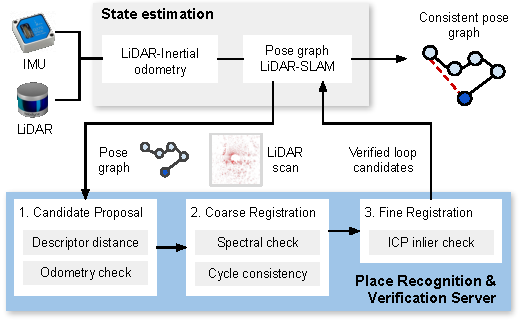
\includegraphics[width=\columnwidth]{pics/method_pipeline.pdf}
  \caption{Our place recognition pipeline. VILENS provides a continuous odometry estimate at 10 Hz. Pose graph SLAM is used to optimize poses after successful loop closure verification. 
  The place recognition module consists of three steps: Loop candidate proposal, coarse registration, and fine registration. We verify loop candidates
  at the global descriptor-level, local feature-level consistency, and finally fine registration level. A loop candidate is integrated in the pose graph only if it passes these three stages.}
  \label{fig:pipeline}
\end{figure}


% Overall Pipeline
% This star removes this subsection from the A,B,C list. Such that the task A,B,C match
\section{Place Recognition \& Verification Server} \label{sec:pipeline}\haedam{reference to method figure which step is which}
Our place recognition pipeline consists of three steps: loop candidate proposal, coarse registration, and a final fine-registration. At each step, we perform appropriate checks to filter out incorrect loop closures.

The main inputs are the pose graph, with corresponding LiDAR scans attached to each pose, as well as the single query scan. The query scan is provided by different sources depending on the task we are solving. For example, in the relocalization task it will be a live scan directly from the LiDAR sensor. Further details are provided in the corresponding sections.

% 1.1 Descriptors (Descriptor distance,)
\subsection*{\textbf{Step 1: Loop candidate proposals}}
\label{subsubsec:loop-candidate}
Initial loop closure candidates are obtained by comparing global descriptors extracted from the pose graph scans as well as the query scan. In this paper, we evaluate four state-of-the-art methods for descriptor extraction: the learning-based Logg3dNet~\cite{vidanapathirana2022icra} and EgoNN~\cite{komorowski2022ral}, as well as the handcrafted ScanContext~\cite{kim2018iros} and STD~\cite{yuan2023icra}.

Given the reference pose graph and the query scan, we compute a database of descriptors using all the scans in the pose graph, given by the matrix $\mathbf{D} \in \R{N\times M}$, where $N$ is the number of poses in the pose graph and $M$ the descriptor dimension. Additionally, we compute the descriptor for the query scan, denoted by $\mathbf{d}_{q} \in \R{M \times 1}$. 

To obtain candidates, we simply compute the pairwise distances of the scan to the database using the cosine similarity:
\begin{equation}
  \mathbf{S} = \mathbf{D} \cdot \mathbf{d}_{q} \in \R{N \times 1}
\end{equation}
The vector of descriptor distances $\mathbf{S}$ is sorted by increasing distance, and only the top-$k$ candidates are selecting using a distance threshold $\tau_{s}$.

\mfallon{we should discuss this comment here - I dont know what it means:}
If a spatial prior is available, for example from LiDAR-inertial odometry, we also perform an additional spatial check discarding all the candidates that are more than \SI{20}{\meter} away from the query scan. The output is a set of candidate nodes $\{ n_c\}$.

% 2.1 Pose Estimation (RANSAC) ... notation is a bit confusing.
\subsection*{\textbf{Step 2: Coarse Registration}}
\label{subsubsec:coarse-registration}
Next, we estimate the relative 6DoF transformation that expresses the pose associated to the query scan w.r.t each candidate node, which we denote $\Delta \mathbf{T}$. For the handcrafted methods (ScanContext and STD), the relative transformation is directly an output of descriptor computation. For the learning-based approaches, we use the point-wise feature vectors outputted in the forward pass of Logg3dNet and EgoNN for point matching, which is used in a RANSAC-based pose estimation scheme~\cite{fischler1981ransac} to obtain the estimated relative transformation.

% \mfallon{please search for `relative' thoughout the paper and check that you use `relative transformation' not `relative pose'.}

% 2.2 SGV
We additionally verify the inlier matches using the \emph{Spectral Geometric Verification}~\cite{vidanapathirana2023ral} method, which provides an additional measure of the quality of the feature matches.

Lastly, we carry out a \emph{cycle consistency} verification, which checks whether the relative transformations between pairs of nodes are mutually consistent with one another. In brief, when given four pose graph nodes $n_i, n_j, n_k, n_l$, we test how close the following equivalence holds:
\begin{equation}
\Delta\mathbf{T}_{i,j}\, \Delta\mathbf{T}_{j,k}\, \Delta\mathbf{T}_{k,l}\, \Delta\mathbf{T}_{l,i}\, \approx \mathbf{I}_{4\times4} 
\end{equation}
If the difference around a cycle is more than a threshold of \SI{10}{\centi\meter} and \SI{1}{\degrees} we reject the candidate. This is shown in \figref{fig:cycle-consistency}, please refer to the corresponding sections for further details.

The interpretation of these transformations change if we discussing online SLAM (\secref{sec:online_slam_mode}), offline multi-mission SLAM (\secref{sec:offline}), or pure relocalization (\secref{sec:relocalization}). 

\begin{figure}[t]
  \centering
  \includegraphics*[width=\columnwidth]{pics/methods_pairwise_consistency.pdf}
  \caption{Our proposed cycle consistency check is general and applies to the online and offline multi-mission SLAM case, as well as relocalization tasks. We only need the relative transformation estimates and loop candidates between four nodes $n_i, n_j, n_k, n_l$ to verify the validity of a loop. Please refer to \secref{subsubsec:coarse-registration} for technical details.}
  \label{fig:cycle-consistency}
\end{figure}

% 3. ICP 
\subsection*{\textbf{Step 3: Fine Registration}}
\label{subsubsec:fine-registration}
Finally, we employ the Iterative Closest Point (ICP) algorithm~\cite{besl1992icp} for fine registration of the proposed candidates. We use the \emph{libpointmatcher} implementation~\cite{pomerleau2013iros}, which also provides information on the quality of the registration, such as the proportion inlier points and the Residual Error of each point to access the alignment.
% \mfallon{LibPM returns the residual error of each point. My code uses a threshold (20cm) to determine if a point is an inlier. This magic number is really undertuned}
% this magic number of 20cm is very very important:
% https://github.com/ori-drs/vilens/blob/develop/icp_odometry/icp_odometry/src/icp_odometry/registration_verification.cpp#L28

% since the number of points is fixed (20k I think), the number is really a proportion
We use the proportion of inliers and the residual error of \SI{20}{\centi\meter} as a final verification step to reject loop candidates. The verified candidates are then used for SLAM or relocalization tasks, which are detailed in the following sections.

\section{Task A: Online Single-mission SLAM} 
\label{sec:online_slam_mode}
\begin{figure}[t]
  \centering
  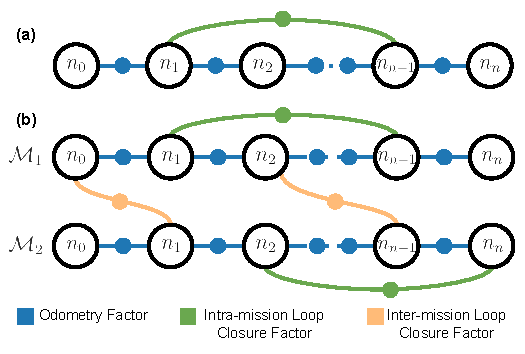
\includegraphics[width=0.99\columnwidth]{pics/factor_graph_v2}
  \caption{Pose graph formulation used for (a) online, and (b) offline multi-mission SLAM optimization. Each node $n_{i}$ has a 6DOF pose $\mathbf{x}_{i}$, which correspond to the main variables estimated on each case.}
  \label{fig:factor_graph}
\end{figure}

The first task we consider is LiDAR-based online SLAM. Our implementation defines it as an incremental pose graph estimation problem (see \figref{fig:factor_graph},(a)). Consider consecutive loop closures at nodes $n_{i}$, $n_{i+1}$ and $n_{j}$, $n_{j+1}$. Edges are provided by relative estimates from our LiDAR-inertial odometry system (odometry factors, denoted by $\Delta\mathbf{T}_{i,i+1}, \Delta\mathbf{T}_{j, j+1}$), and verified loop closure candidates from our place recognition server (loop closure factors, $\Delta\mathbf{T}_{i+1, j}, \Delta\mathbf{T}_{i, j+1}$).
\mfallon{a pose graph is a type of factor graph. no need to say factor graph here}

For the cycle consistency verification described in \secref{subsubsec:coarse-registration}, we consider the relative transformation change between consecutive loop closure candidates w.r.t the pose graph poses and the odometry change (\figref{fig:cycle-consistency}  $i$, $j$, $k$, $l$, replaced by ${i}$, ${i+1}$, ${j}$, ${j+1}$). Again, a cycle consistency needs to be satisfied:
\begin{equation}
  \label{eq:cycle-online}
  \Delta\mathbf{T}_{i,i+1}\, \Delta\mathbf{T}_{i+1, j}\, \Delta\mathbf{T}_{j, j+1}\, \Delta\mathbf{T}_{i, j+1}^{-1} \approx \mathbf{I}_{4\times4}
\end{equation}
\haedam{exp:cycle consistncy works well in this scenario,}
\section{Task B: Offline Multi-Mission SLAM}\label{sec:offline}
Offline multi-mission SLAM addresses the challenge of merging multiple pose graph SLAM missions ${\mathcal{M}_{1, \ldots, n}}$, collected over time, with partly overlapping area. 
The goal is to find inter-mission loop candidates to construct a unified map in a common reference frame. This application is relevant for forestry applications, where it is required to map larger areas by integrating surveys conducted over multiple missions or campaigns.

Unlike the scenario of on-road navigation, where similar routes (hence locations) are revisited, we considered off-road scenarios where the missions are collected in dense forests, where it is often unfeasible to retrace the same paths on each sequence. To avoid inefficiently retracing our steps, we wish to identify loop candidates when passing no closer than about \SI{10}{\meter}, providing the flexibility needed to merge two roughly overlapping missions.

Each mission ${\mathcal{M}_{i}}$ is defined by a pose graph with odometry factors and intra-mission loop closures, obtained during each independent online SLAM run. We aim to provide additional \emph{inter-mission} loop candidates that bridge nodes across missions, as shown in \figref{fig:factor_graph} (b). In this case, loop candidates are obtained by incrementally matching each mission of the nodes on matched missions and corresponding LiDAR scans across the missions.
\mfallon{do you actually do all-v-all? I incrementally build the database graph so its 1v1 and then 2v2.}
\haedam{you're right, we incrementally build it }
For the loop proposal step, we executed the same procedures described in \secref{subsubsec:loop-candidate}, but with the stringent descriptor distance threshold $\tau_{s}$. We observed that in the multi-session case, this was required to allow a larger set of candidates that were later verified by stronger procedures such as the cycle consistency check. 
For the cycle consistency step, we considered pairs of nodes within the same mission, namely $n_i, n_j \in \mathcal{M}_1$ and $n_k, n_l \in \mathcal{M}_2$. The intra-mission relative transformation were then $\Delta\mathbf{T}_{i,j}, \Delta\mathbf{T}_{k, l}$, while the inter-mission relative transformations between loop candidates were given by $\Delta\mathbf{T}_{i,k}, \Delta\mathbf{T}_{j,l}$:
\begin{equation}
  \label{eq:cycle-offline}
  \Delta\mathbf{T}_{i,j}\, \Delta\mathbf{T}_{j,l}\, \Delta\mathbf{T}_{k, l}^{-1}\, \Delta\mathbf{T}_{i,k}^{-1}\, \approx \mathbf{I}_{4\times4}
\end{equation}

\section{Task C: Relocalization} \label{sec:relocalization}
Lastly, we considered the case in which a prior map of the forest was available (from online SLAM). Our place recognition \& verification server could then be used as a relocalization module, by using the loop candidate proposals to produce initial pose estimates, then coarese-to-fine registration achieving real-time localization of the LiDAR sensor base $\B$ with the prior map's coordinate frame $\M$, denoted by $\mathbf{T}_{\M\B}$.

\mfallon{the following paragraph is confusing and poorly written. If we are doing cycle consistency checking we don't have a `successful relocalization' we only have a `possible candidate'}
\mfallon{can you try again?}
\haedam{Okay, I add a sentence above and below}
Similarly to the previous tasks, the main difference is in defining the cycle consistency check. For this case, it is between the current and the last successful relocalization: Given the last relocalization estimate $\mathbf{T}_{\M\B}(t-1)$ and the current estimate $\mathbf{T}_{\M\B}(t)$, we compared the  against the odometry estimates at the same timestamps $\mathbf{T}_{\Odo\B}(t-1)$ and $\mathbf{T}_{\Odo\B}(t)$, where $\Odo$ indicates the fixed odometry frame. The cycle consistency check is then defined as:

\begin{equation}
  \label{eq:cycle-relocalization}
  \underbrace{\mathbf{T}_{\M\B}(t)^{-1}\, \mathbf{T}_{\M\B}(t-1)}_{\Delta\mathbf{T} \text{ in $\M$ frame}}  \, \underbrace{ \mathbf{T}_{\Odo\B}(t-1)^{-1}\,  \mathbf{T}_{\Odo\B}(t)}_{\Delta\mathbf{T} \text{ in $\Odo$ frame}} \approx \mathbf{I}_{4\times4}
\end{equation}
This check is used to verify the relocalization estimate, and if successful, ICP is used to fine-localize the LiDAR sensor within the prior map.
\mfallon{again, we need to point out that localisation into a giant point cloud map would be very inconvenient.}

This relocalization capability facilitates various applications, such a enabling a harvester robot to operate autonomously within a prior map or enabling foresters to visualize a rendering of the virtual forest along with important information on a screen in real-time. An example demonstrating this capability is later presented in \secref{sec:exp_relocalization}, where a prior map of the forest is generated using a backpack-based LiDAR mapping system, and a legged robot continuously relocalizes itself within that prior map as part of an inspection task.
\mfallon{please don't over claim - we didnt do this. soften your comments here please}

\mfallon{But Matias: it would be awesome to do what is described here!}
\haedam{I will try this experiment and see if it works.}

\chapter{Experiments}
\label{chapter:experiments} 

% \section{Experimental Evaluation Overview}\label{sec:exp}
In this section, we rigorously evaluate our place recognition pipeline to assess its performance in dense forest environments. Our evaluation includes four distinct test sites featuring varying forest compositions: Evo (Finland) characterized by coniferous trees; Stein-Am-Rhein (Switzerland) Wytham Woods (UK) and Forest of Dean (UK) containing both broad-leaf and coniferous tree species. We evaluate all three operational modes of our system: Online SLAM, Offline Multi-Mission SLAM, and Relocalization.
% We can remove the summary of experiments to save space if needed
The experiments conducted are as follows:
\begin{enumerate}[label=\Roman*.]
  \item Evaluation of four different place recognition models at the descriptor-level, tested across multiple forest environments with different LiDAR setups. (\secref{sec:exp_desc_analysis}) 
  \item Performance assessment during both online and offline SLAM operations within dense forest settings. (\secref{sec:exp_online_slam} \& \secref{sec:offline_multi_mission}).
  \item Analysis of successful loop closures, based on baseline distance and orientation differences. (\secref{sec:exp_online_slam})
  \item Demonstration of the relocalization application in a previously mapped forest environment, showcasing its utility in an inspection task performed by a quadruped robot. (\secref{sec:exp_relocalization})
\end{enumerate}

\begin{figure}[htbp]
  \centering
  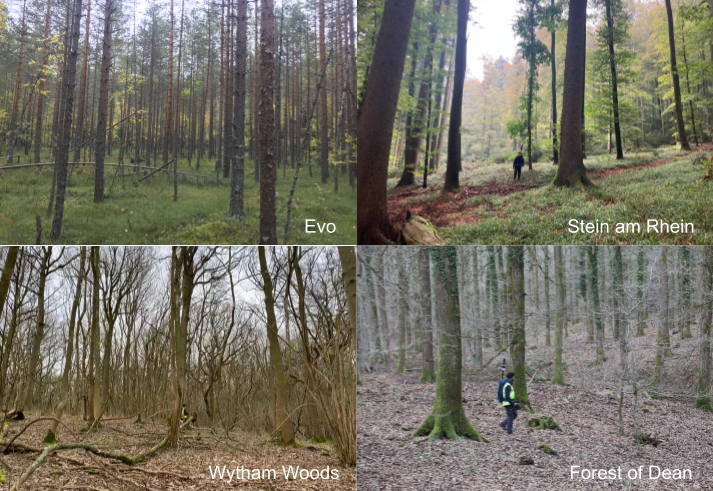
\includegraphics[width=\columnwidth]{pics/exp_0_missions_dataset.pdf}
  \caption{Illustrative examples of four forests used in the experiments. From top left to bottom right: Evo (Finland, May), Stein am Rhein (Switzerland, Sep), Wytham Woods (UK, Feb), and Forest of Dean (UK, March). The datasets were collected using backpack-LiDAR systems across different seasons and forest types.}
  \label{fig:missions_dataset}
\end{figure}


% First experiment: descriptors
\section{Place Recognition Descriptors}
\label{sec:exp_desc_analysis} 
In this experiment, we evaluated the descriptors of four different place recognition models (Logg3dNet, EgoNN, ScanContext, STD) focusing on their ability to accurately capture loop-candidates in forest environments. Logg3dNet and EgoNN models are learning-based methods and were pre-trained on the Wild-Places dataset. 
\subsection*{Datasets}
We collected the dataset with two different LiDAR sensors mounted on a backpack: Hesai XT32 and Hesai QT64  as discussed in previous \secref{sec:system_setup}. Note that Wild-Place\cite{knights2023icra} dataset was collected using a inclined VLP-16 LiDAR mounted on spinning motor. This enabled capturing the canopy of the forest, which is difficult for our backpack LiDAR setup. Below summarises the characteristic of different forests:
\begin{itemize}
  \item \textbf{Evo:} Evo dataset was collected in forests in Finland. The dataset was collected in May using the Hesai XT32 LiDAR sensor. The forest is characterized by tall coniferous trees with medium tree density.
  
  \item \textbf{Stein am Rhein:} Stein am Rhein dataset was collected in a forest in Switzerland in October. The dataset was collected using the Hesai XT32 LiDAR sensor. It displays mixed species and bushes with a low tree density.   

  \item \textbf{Wytham Woods:} Wytham Woods dataset was collected in a densely wooded area in the UK in February. The dataset was collected using the Hesai QT64 LiDAR sensor. It is characterized by a high tree density with complex terrains featuring hills and valleys.
  
  \item \textbf{Forest of Dean:} Forest of Dean dataset was collected in a forest in the UK in March. The dataset was collected using the Hesai QT64 LiDAR sensor. The dataset displays a sparser plantation with a low tree density. 

  \item \textbf{Wild-Place:} Wild-Place dataset was collected in a forest in Australia over different seasons. The dataset was collected using a VLP-16 LiDAR sensor mounted on a spinning motor. The trajectories were along the open access roads and the forest canopy was captured. The dataset is characterized by a low tree density.  
\end{itemize}

% \begin{table}[ht]
%   \centering
%   \label{tab:lidar_specs}
%   \begin{tabular}{|p{2.5cm}|p{2cm}|p{2.3cm}|p{2.3cm}|c|}
%     \hline
%     \centering \textbf{Location} & \centering  \textbf{LiDAR} & \centering  \textbf{Field of View (\textdegree)} &\centering  \textbf{Effective Range (m)} & \textbf{Tree Density} \\
%     \hline
%     \centering Wild-Place & \centering VLP-16 & \centering 30  & \centering 50 & Low \\
%     \hline
%     \centering Evo &  \centering XT32 &\centering 30 &\centering 50 & Medium \\
%     \hline
%     \centering Stein am Rhein &\centering  XT32 & \centering 30 & \centering 50 & Low \\
%     \hline
%     \centering Wytham Woods &\centering  QT64 &\centering 100 &\centering 30 & High \\
%     \hline
%     \centering Forest of Deans &\centering QT64 &\centering 100 &\centering 30 & Low \\
%     \hline
%   \end{tabular}
% \caption{Datasets and LiDAR specifications.}
% \end{table}


\begin{table}[htbp]
  \centering
  \caption{Evaluation running for a sequence of dataset.}
  \label{tab:eval_sequence}
  \small
  \centering
  \begin{tabular}{>{\centering\arraybackslash}m{1.5cm} >{\centering\arraybackslash}m{1.5cm} >{\centering\arraybackslash}m{1.5cm} >{\centering\arraybackslash}m{1.5cm} >{\centering\arraybackslash}m{1.5cm} >{\centering\arraybackslash}m{1.5cm} >{\centering\arraybackslash}m{1.5cm}}
  \toprule
  Dataset  & Eval Modes & Avg. Mapping area(ha) & Avg. Duration (min) & Avg. \#Indiv. pc  & Avg.\#points per indiv.pc  \\
  \midrule
  Evo  & Desc. Online. Offline. & 0.74 ha   & 24 min & 969 &  110k \\
  \midrule
  Stein am Rhein  & Desc. & 0.27 ha & 13 min & 363 &  120k \\
  \midrule
  Wytham Woods & Desc. Online. Offline.  & 1.2 ha & 22 min& 707 & 55k \\
  \midrule
  Forest of Deans & Online. Offline. Reloc. & 0.45 ha  & 17 min & 649 & 50k \\
  \midrule
  Wild-Place & Desc. & Perimeter 3.17km  & 48 min & 5805 & 300k \\
  \bottomrule
  \end{tabular}
\end{table}

\subsection*{Precision-Recall Curves}
Precision-recall curves (See \figref{fig:pr_curves}) show how accurately (precision) and frequently (recall) each  model detects correct loop candidates within a reasonable distance threshold (here set to 10\,m) at various descriptor thresholds $\tau_{s}$ in four different forests. Among positive candidates   (whose descriptor distance < $\tau_{s}$ ), we classify them into true positive(\emph{TP}) and false positive(\emph{FP}) depending on whether the candidate is actually located within the loop-closure distance threshold, 10 meter. 
Similarly, among negative candidates, we classify them into true negative(\emph{TN}) and false negative(\emph{FN}) depending on their true location. Thus:
\[ Precision = \frac{TP}{TP + FP} \quad   \ Recall = \frac{TP}{TP + FN} \]

From the precision-recall curves (\figref{fig:pr_curves}), it is evident that Logg3dNet consistently outperforms the other models across the four different forests. Particularly, on the Evo and Stein am Rhein datasets, where a longer range with narrow field of view Hesai XT32 LiDAR was employed, Logg3dNet showed the best performance both in terms of precision and recall, without experiencing any sudden drops in precision.
In contrast, ScanContext demonstrates a significant decrease in precision, attributed to a limited vertical field of view of LiDAR sensor. In more challenging scenarios such as Wytham Woods characterized by complex terrains featuring hills and valleys with dense tree clutter captured with a wide field of view QT64 LiDAR, handcrafted models show a notable decline in performance. However, Logg3dNet remains robust, successfully retrieving a substantial portion of correct loop-candidates, achieving a 70\% precision at a 50\% recall rate. 
\begin{figure}[htbp]
  \centering
  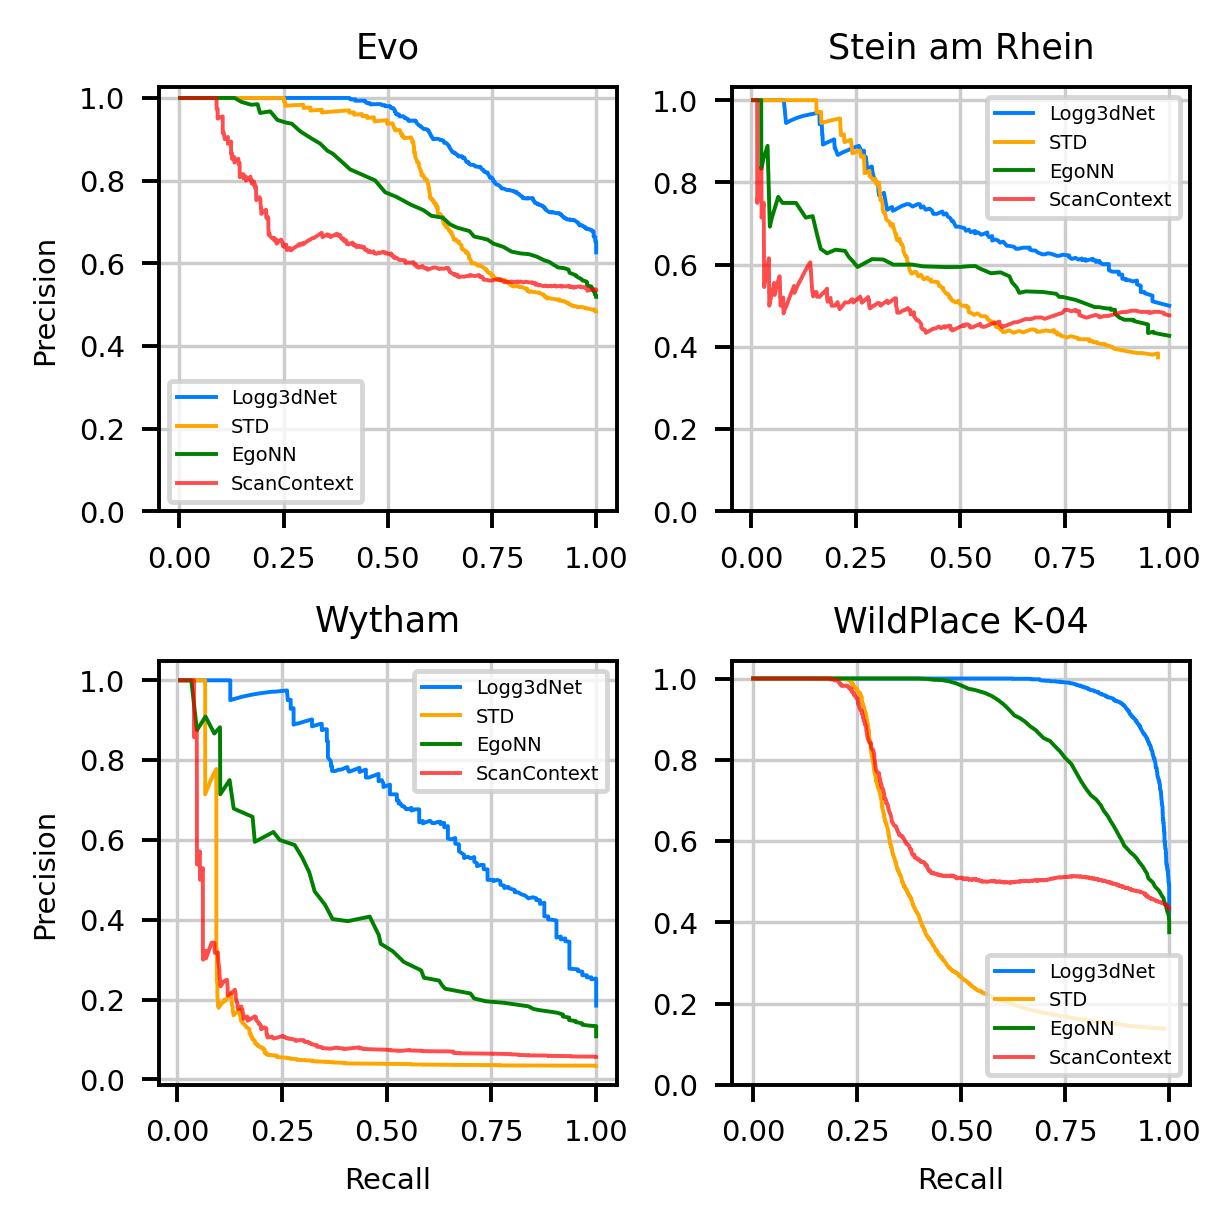
\includegraphics[width=0.9\linewidth]{pics/exp_1.1_pr_curves}
  \caption{Precision-recall curves on four different forest datasets. Evo (Finland, May), Stein am Rhein (Switzerland, Oct), Wytham woods (UK, Feb), Wild-Places \cite{knights2023icra} (Australia).
  Evo and Stein am Rhein datasets were collected by Hesai XT32, and Wytham woods dataset was collected by Hesai QT64. Datasets were collected by backpack-LiDAR within dense forests. Only top-1 candidate within 10\,m of the ground truth position is regarded as a true positive candidate.}
  \label{fig:pr_curves}
\end{figure}
% \mfallon{I get to this bit and there is just a hole in the work because nothing about Logg3dNet's algorithm is ever discussed. There is no tuning or ablation. It just presented `as is'.}
\subsection*{Heatmaps}
To further analyze the distinctiveness of each descriptor, we measured the descriptor distances between all query and database descriptors. This is shown in \figref{fig:heatmap_evo12} as a heatmap, which provides a visual representation of the discriminative potential of each descriptor. Consistent with the precision-recall curves, Logg3dNet descriptors exhibited higher similarity with the ground truth heatmap as observed in the highlighted areas, indicating a high true-positive rate and low false-positive rate, respectively. This implies that Logg3dNet descriptors can effectively detect corresponding loop-candidates during revisits, whereas EgoNN and ScanContext tend to be less discriminative, often returning numerous false-positive candidates. Based on this evidence, we chose Logg3dNet as main the place recognition method for the rest of the experiments.
\begin{figure}[htbp]
  \centering
  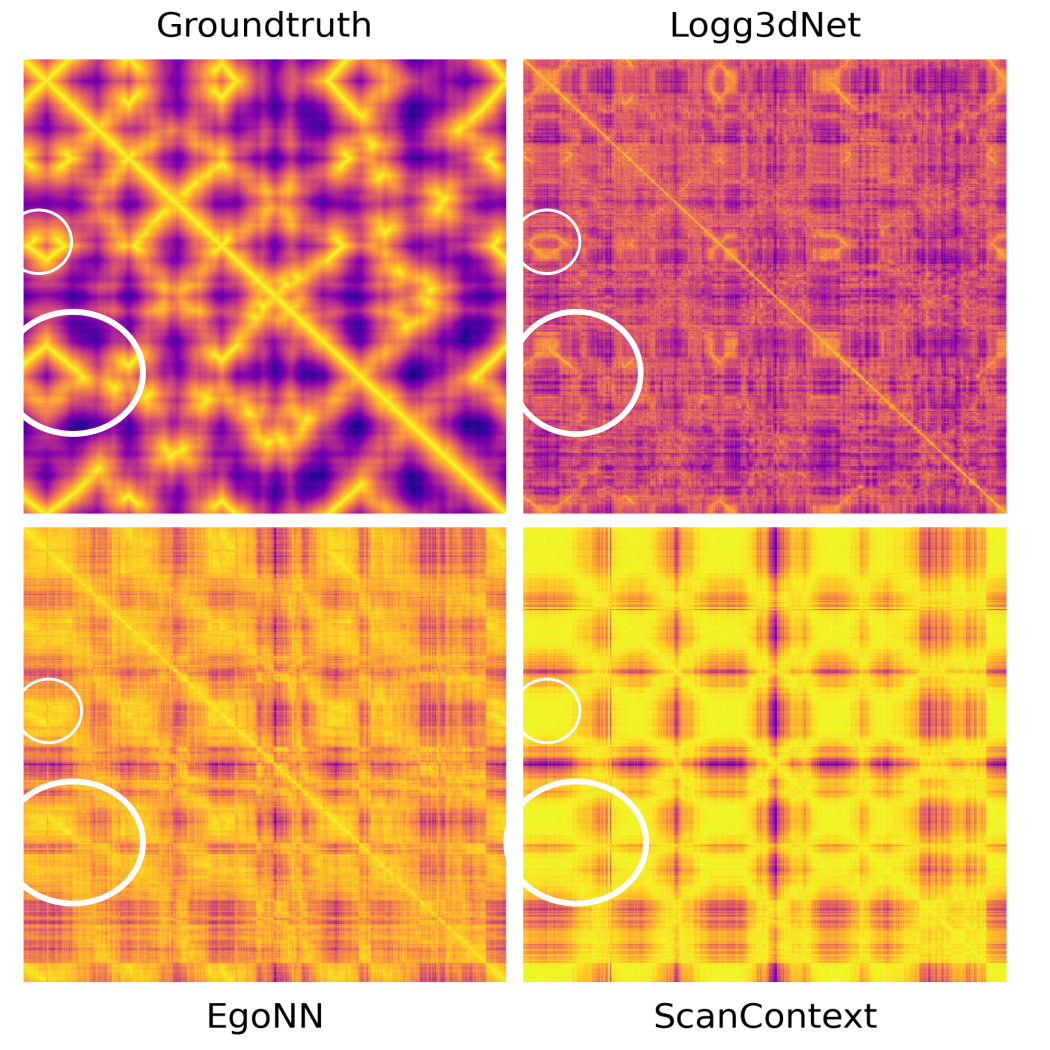
\includegraphics[width=0.9\linewidth]{pics/exp_1.2_heatmap_evo12_plasma_edit}
  \caption{Heatmaps depicting descriptor distances for the Evo dataset. Yellow hues denote a high descriptor similarity between scans, whereas purple indicates the low similarity. Patterns more closely resembling the ground-truth (top-left) indicate better descriptor performance. Logg3dNet descriptors shows the most similar patterns, whereas ScanContext descriptors are least discriminative among these models. We use $\tau_{s}$ that corresponds to the $F_1$-max score in evaluation.}
  \label{fig:heatmap_evo12}
\end{figure}





%%% Second experiment: Online SLAM
\section{Online Single Mission SLAM}
\label{sec:exp_online_slam}
In this experiment, we investigate the online place recognition capability of our system, wherein loop closures from the place recognition module are integrated into the SLAM system. The database $D$, is incrementally built as the sensor moves through the environment. When matching, we exclude the most recent 30 seconds of data to prevent loop closures with immediately recent measurements.
\begin{figure}[htbp]
  \centering
  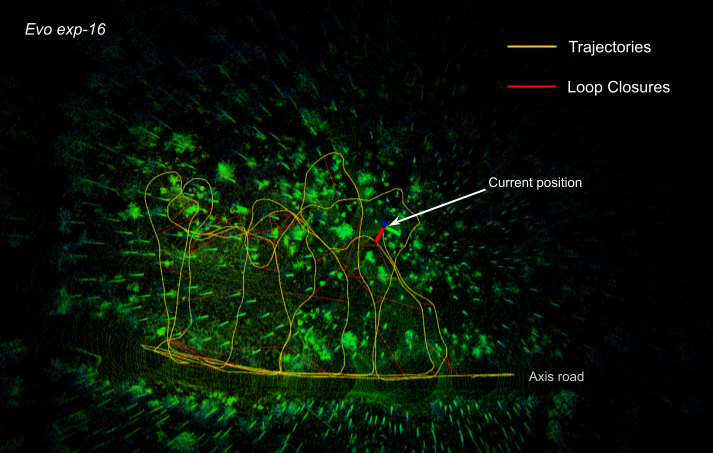
\includegraphics[width=0.9\columnwidth]{pics/exp_2_0_rviz.png}
  \caption{Online SLAM Operation visualizations through Rviz on Evo exp16 sequence. }
  \label{fig:exp_2_0_rviz}
\end{figure}



\subsection*{Online Place Recognition}
% Interpret results exp_2_1
\figref{fig:exp_2_1_evo_online} presents an illustrative example of online SLAM performance on the Evo datasets, depicting the sets of loop candidates after each verification step. Initially, many loop closure candidates are proposed (shown in blue) under a descriptor matching threshold $\tau_{s}$ of $F_1$-max score. Loop closures beyond a conservative estimate of \SI{20}{\meter} are rejected using the odometry information. After this, a subset of loop closure candidates are identified using RANSAC matching (highlighted in orange), and finally, a refined set of loop closures that pass the consistency and ICP steps are integrated into the SLAM framework. Final loop closures (shown in red) are one of ICP verified loop candidates by checking pose graph density to avoid over-constraining the pose graph. We tested on two sequences on Evo and Wytham dataset. 
\newline
\textbf{Evo}\hspace{0.5em} We tested on Evo dataset as shown \figref{fig:exp_2_1_evo_online}. Evo16 sequence is densly scanned where each zigzag turn is about 10-15m apart, whereas Evo12 is mapped sparsely with about 20-30m apart. For Evo16, we can observe frequent loop candidates upto \SI{20}{\meter} between each zigzag turn, whereas for Evo12, loop closures are less frequent and more candidates (above \SI{15}{\meter}) are strongly rejected before RANSAC registration(Blue lines). In summary, we observed that the system can reliably detect loop closures inside the dense forest in both cases and correct the drift. 
\begin{figure}[htbp]
  \centering
  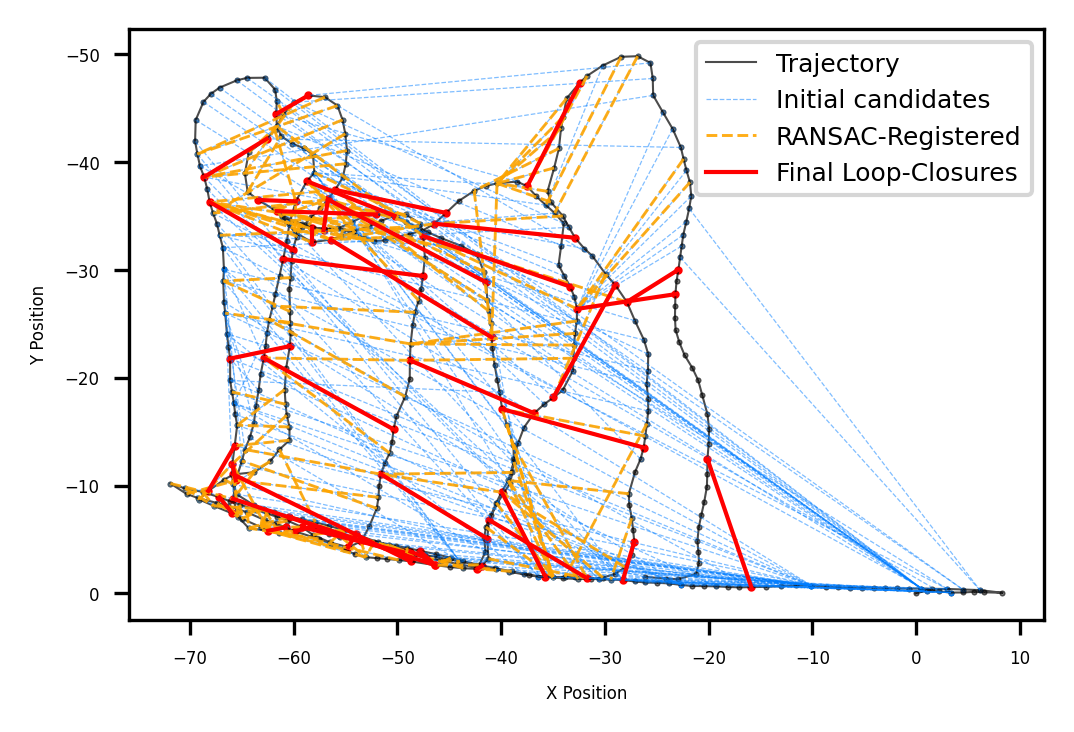
\includegraphics[width=0.54\columnwidth]{pics/exp_2_1_evo16_online2.png}
  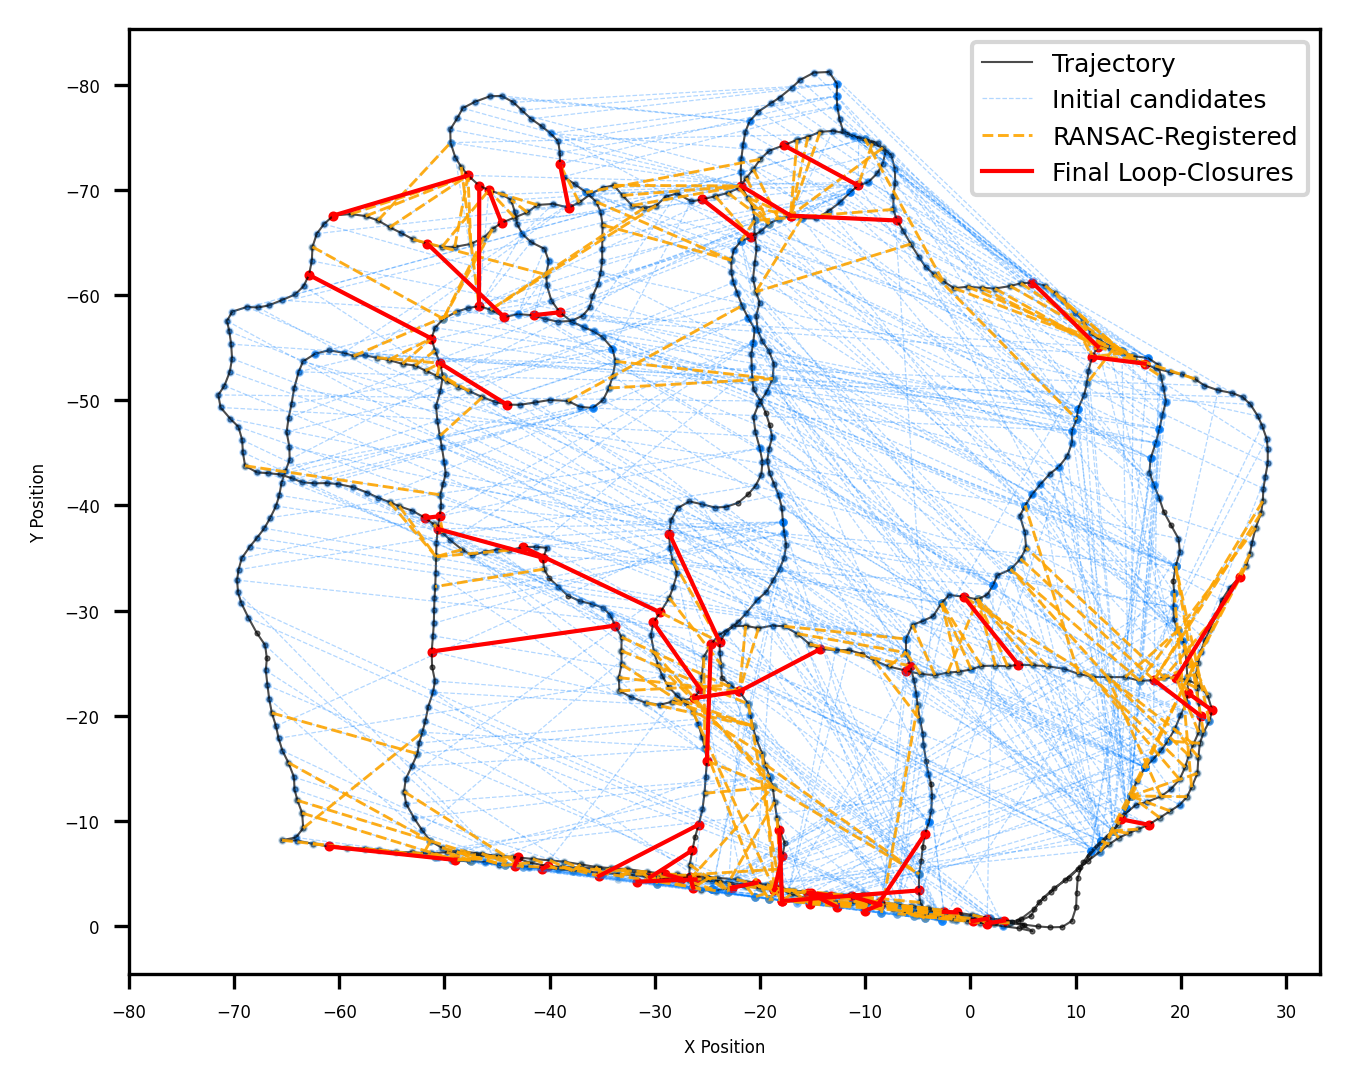
\includegraphics[width=0.44\columnwidth]{pics/exp_2_1_evo12_online.png}
  \caption{Online SLAM results on Evo dataset. Evo16(Left) and Evo12(Right). Initial candidates (Blue) proposed by descriptor distance and odometry check. Yellow lines are successfully RANSAC-registered candidates which passed SGV and pairwise consistency checks. Red lines are final loop closures after ICP verification and checking constraints density in pose graph.}
  \label{fig:exp_2_1_evo_online}
\end{figure}
\newline
\textbf{Wytham Woods}\hspace{0.5em} We further tested on more challenging dataset, Wytham Woods, which is a densely wooded area with uneven terrain, including hills. In \figref{fig:exp_2_1_ewytham_online}, we observed that there are still enough numbers of correct RANSAC-registered loop candidates, but ICP could not fine-register them. For example, regarding Mission D(top figure) of \figref{fig:exp_2_1_ewytham_online}, our system correctly detected loop candidates and RANSAC registered them (Yellow lines) at each turns. However, the ICP rejected almost all candidates due to very small number of overlapping point clouds between two scans (usually 2k-3k out of 20k points, $\sim$\SI{10}{\percent} overlaps). Unfortunately, lowering ICP thresholds to less than $\sim$ 3k points resulted in failure of system. Our system suffers from high outliers rate due to occlusions and sparse point clouds at the far distance making ICP registration challenging. As a result, our system partly corrected the drifts in both sequences, failing to correct drifts at the start. 
\begin{figure}[htbp]
  \centering
  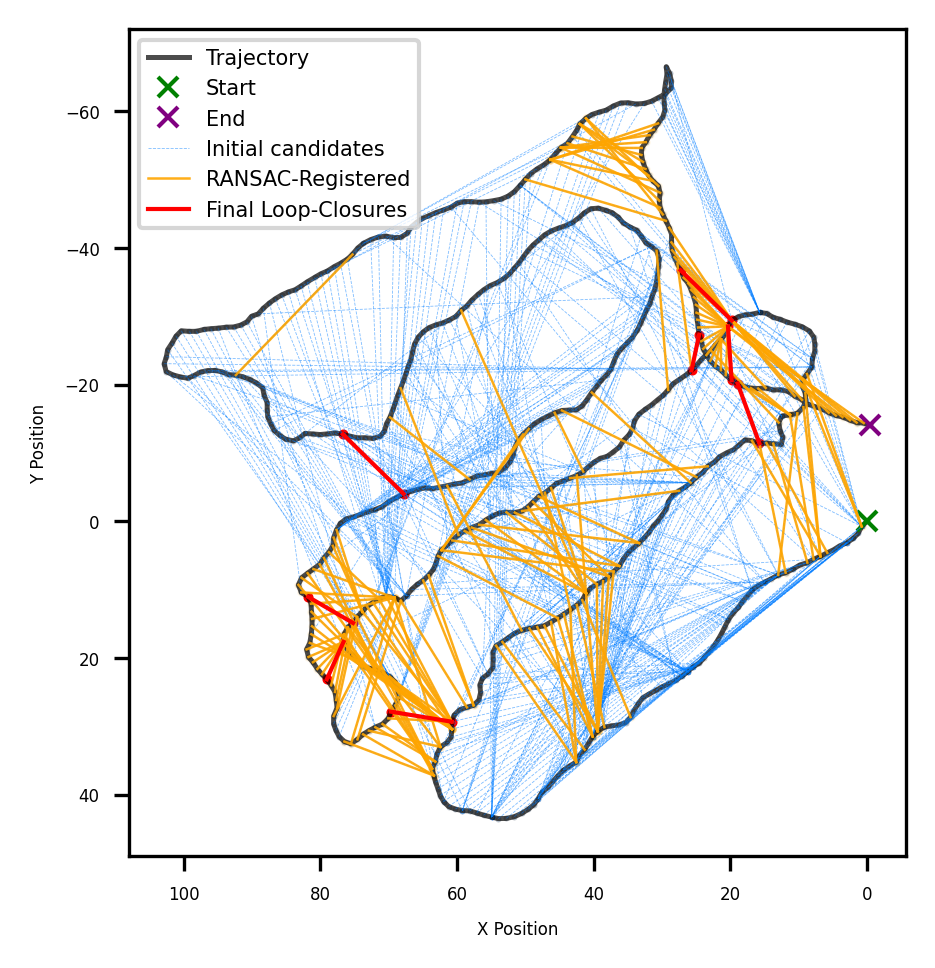
\includegraphics[width=0.49\columnwidth]{pics/exp_2_1_wytham_D.png}
  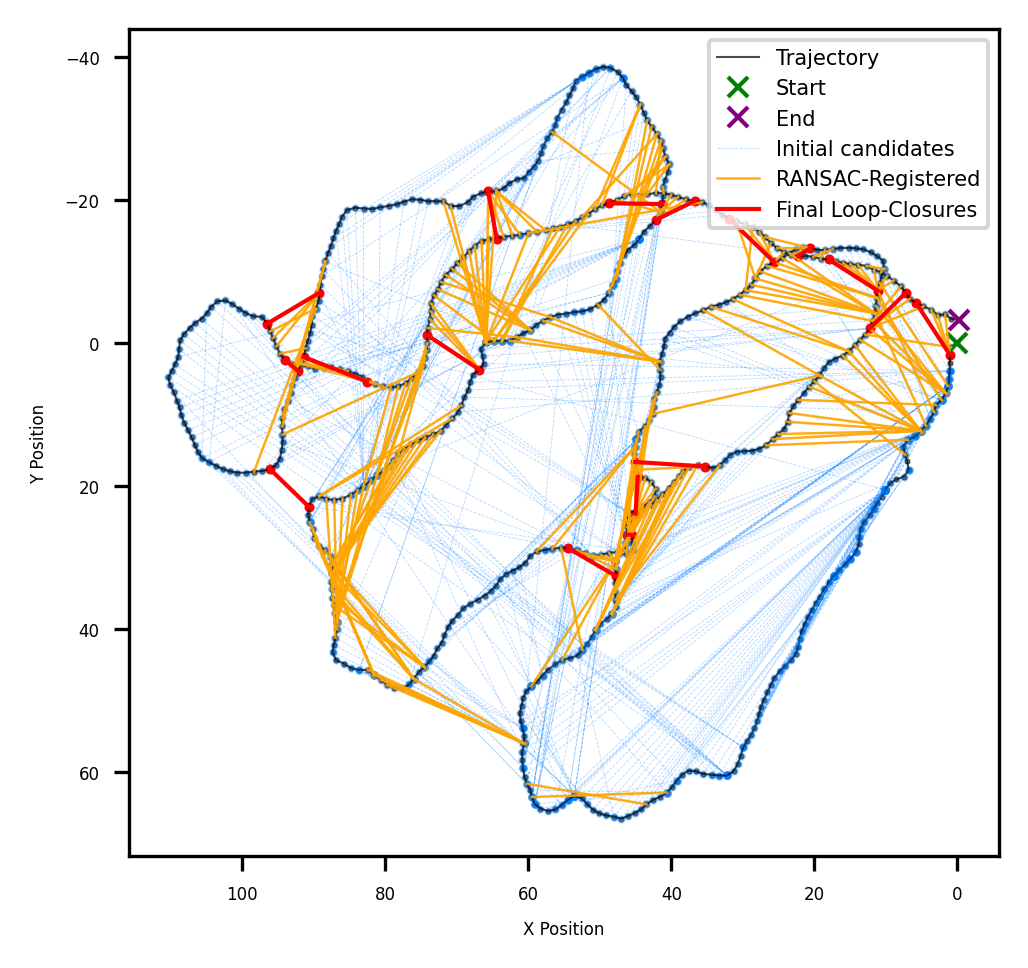
\includegraphics[width=0.49\columnwidth]{pics/exp_2_1_wytham_C.png}
  \caption{Online SLAM results on Wytham Woods, two sequences Mission D(Left) and Mission C(Right) are shown. Blue lines are initial candidates proposed by descriptor distance and odometry check. Yellow lines are successfully RANSAC-registered candidates which passed SGV and pairwise consistency checks. Red lines are final loop closures after ICP verification and checking constraints density in pose graph.}
  \label{fig:exp_2_1_ewytham_online}
\end{figure}


\subsection*{Loop Closure Statistics}
% Present results in exp2_2
Alongside visual illustrations of loop closures, we conducted a comprehensive analysis of loop closure statistics based on distance and viewpoint angles, shown \figref{fig:exp_2_2_loop_closure_histograms}. Our findings show that the system can successfully identify loop closure pairs across considerable baseline distances (\SIrange{10}{20}{\meter}). 
\newline
\textbf{Baseline distance}\hspace{0.5em} We observed that despite the large baseline, a significant portion of initial candidates can be registered using RANSAC-based matching, indicating that the correspondences are accurate. However, the proportion of candidates verified by ICP decreases as the distance between scans increases. Specifically, when scans are \SI{10}{\meter} apart, $\sim$\SI{60}{\percent} of RANSAC-registered candidates are successfully verified by ICP, and when \SI{15}{\meter} apart, only $\sim$\SI{40}{\percent} remains verified. This decrease is due to the diminishing overlap ratio between corresponding scans with increasing distance, making convergence of ICP challenging. \\
\textbf{Viewpoints difference}\hspace{0.5em} Similarly, in terms of viewpoint orientation difference, we observed that a large proportion of the loop candidates up to \SI{90}{\degree} difference are verified both at the RANSAC-registration and ICP-based checks. However, we observed a degradation of performance over \SI{90}{\degree}, which can be attributed to the occlusions in the scans present at large orientation differences. Nonetheless, despite this degradation, the number of final loop closures integrated into the SLAM system proved to be sufficient for correcting the drift.   

\begin{figure}[htbp]
  \centering
  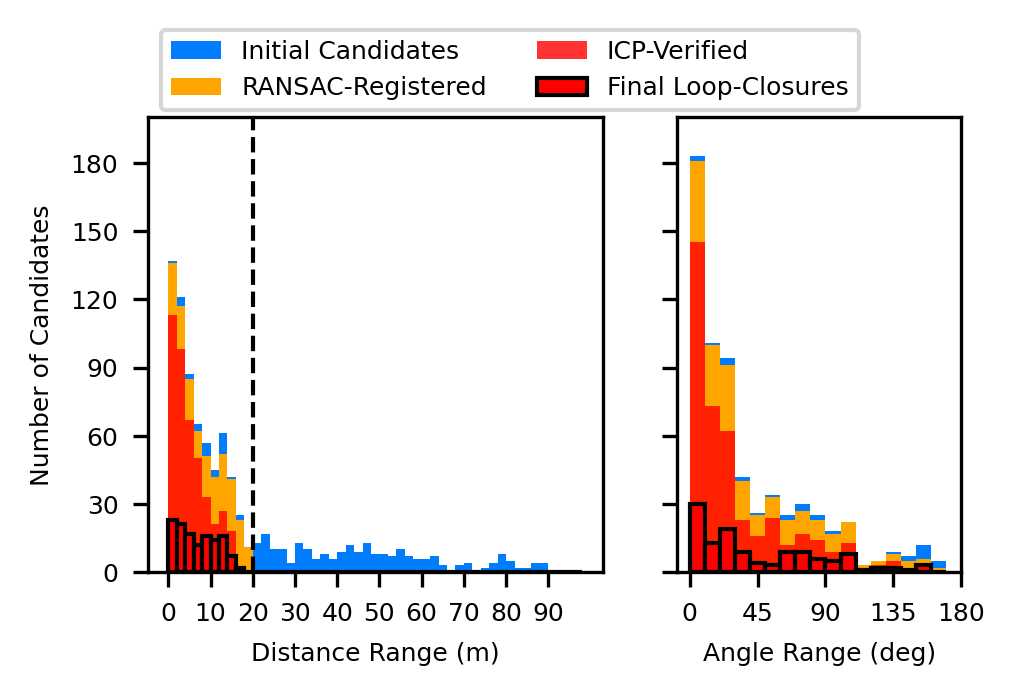
\includegraphics[width=0.85\columnwidth]{pics/exp_2_2_loop_closure_histograms}
  \caption{Loop closures distribution by distance and angle at various stages of the pipeline on Evo dataset.
   Initial candidates based on descriptor distance are shown in blue. Candidates beyond \SI{20}{\meter} are rejected using odometry information. Candidates within \SI{20}{\meter} undergo RANSAC pre-registration with additional verification steps of SGV\cite{vidanapathirana2023ral} and pairwise checks (Yellow). Then these candidates are refined using ICP fine-registration (Red), and final loop closures in the pose graph after checking constraints density in pose graph (red with black outlined).}
  \label{fig:exp_2_2_loop_closure_histograms}
\end{figure}



\subsection*{Model Comparison}
\textbf{ScanContext}\hspace{0.5em} So far we have shown capability of Logg3dNet reliably finding loop closures inside the forest. We now shows ScanContext implemented on our SLAM system on Evo16 dataset to compare with Logg3dNet. It was evident ScanContext shows a drop in performance in \ref{sec:exp_desc_analysis}, and now we evaluate if ScanContext can detect any loop candidates and find 6DoF transformation reliably inside the forest.  
\begin{figure}[htbp]
  \centering
  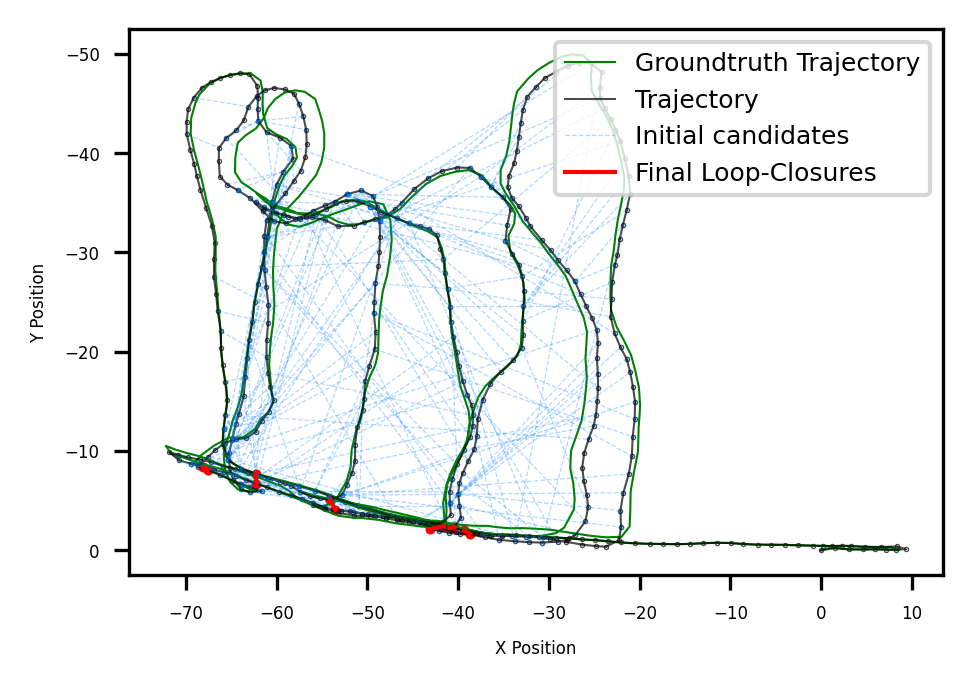
\includegraphics[width=0.75\columnwidth]{pics/exp_2_sc_loop_closure.png}
  % 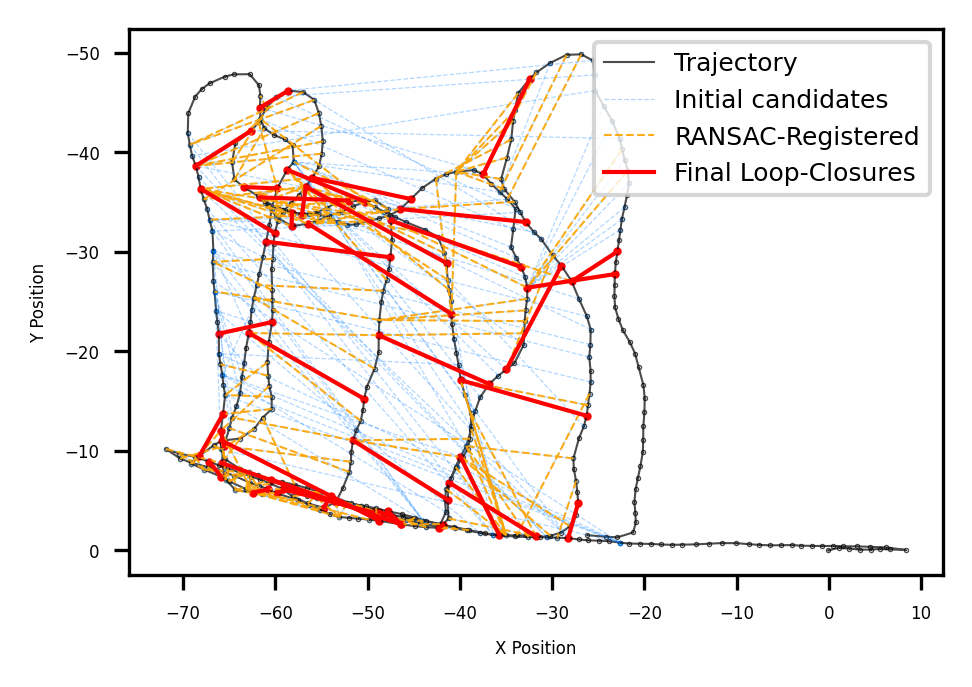
\includegraphics[width=0.49\columnwidth]{pics/exp_2_logg3dnet_loop_closure.png}
  \caption{Loop closures with ScanContext on Evo exp16 dataset. ScanContext could not detect any loop closures inside the dense forest but only in open access roads, whereas Logg3dNet successfully found loop closures inside the forest. Also ScanContext only detected loop closures within 3m(same location), whereas Logg3dNet detected loop closures upto 15m. Finally, Scancontext accumulated drift over time.}
  \label{fig:exp_2_3_loop_closure_comparison}
\end{figure}

From \figref{fig:exp_2_3_loop_closure_comparison}, we can observe that ScanContext could not detect any loop closures inside the dense forest producing very high number of false positives (shown in blue lines), and could detect only in open access roads. Among those loop closures along open access roads, ScanContext detected only within 3m(same location). Finally, Scancontext accumulated drift over time while Logg3dNet corrected drifts. This shows very limited capability of ScanContext compared to Logg3dnet, and this experiment validates the robustness of Logg3dNet compared to ScanContext (handcrafted method) in dense forest environments.



% Third experiment: Offline Multi-Mission SLAM
%%% 
\section{Offline Multi-Mission SLAM} 
\label{sec:offline_multi_mission}
In this experiment, we showcased the ability of our approach to obtain loop closures between different mapping missions and to merge those missions into a common map. In this task, we employed tighter descriptor thresholds ($\tau_{s}$) compared to the online SLAM task, in order to reduce the number of false positive loop candidates.
Below shows the results of merging different sequences within three different datasets: Wytham Woods, Evo, and the Forest of Dean. Each individual mission covers approximately one hectare, with merged map areas ranging from three to five hectares.
\newline
\textbf{Evo, \figref{fig:exp_multi_mission_evo}}\hspace{0.5em} We tested the robustness of our system on the Evo multi-mission dataset, where the XT32 LiDAR was placed at a \SI{45}{\degree} inclination aimed at capturing the forest canopy. Despite the asymmetry in point clouds introduced by this inclination change, which primarily captured points in the forward direction, our approach successfully identified loop closures and achieved multi-mission map merging.
\begin{figure}[htbp]
  \centering
  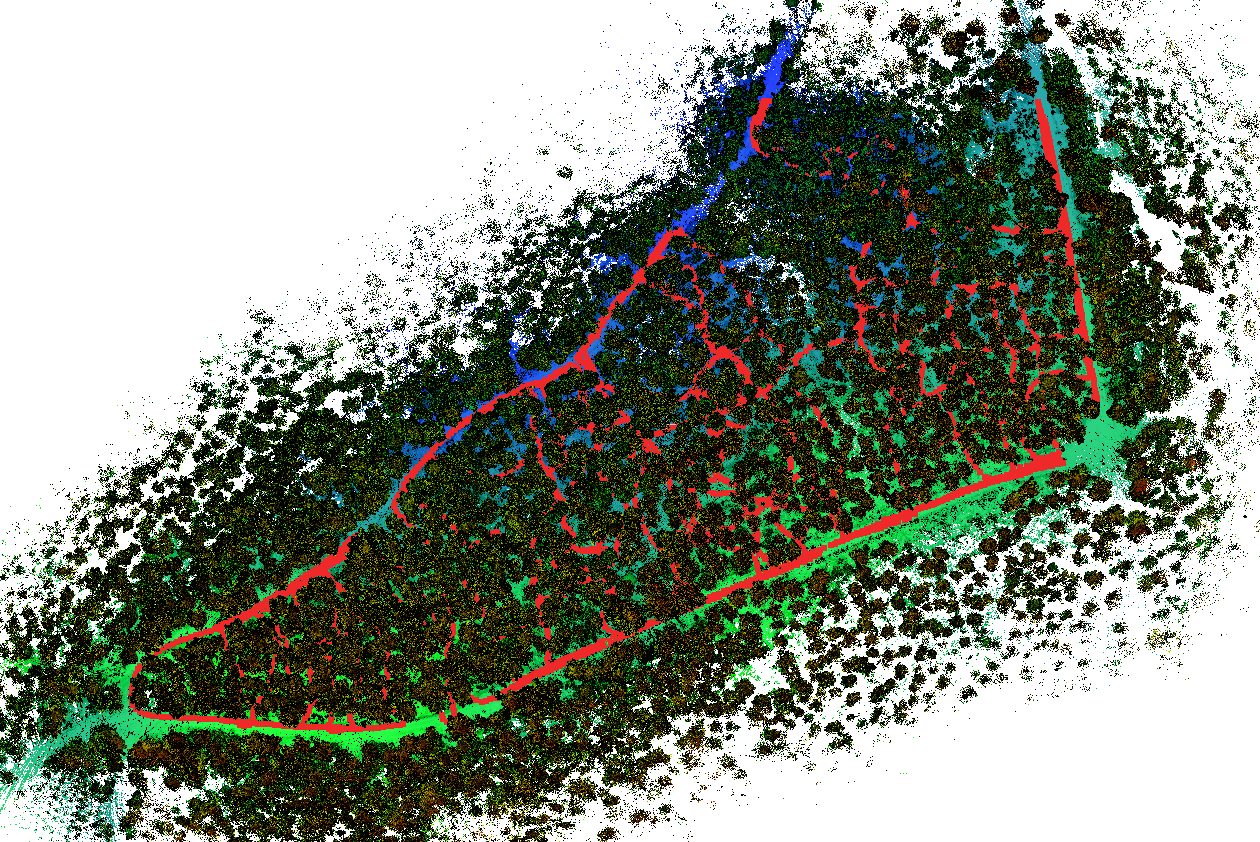
\includegraphics[width=\columnwidth]{pics/exp_3_offline_evo_pcd.png}
  % \caption{Offline multi-mission SLAM point clouds output.}
  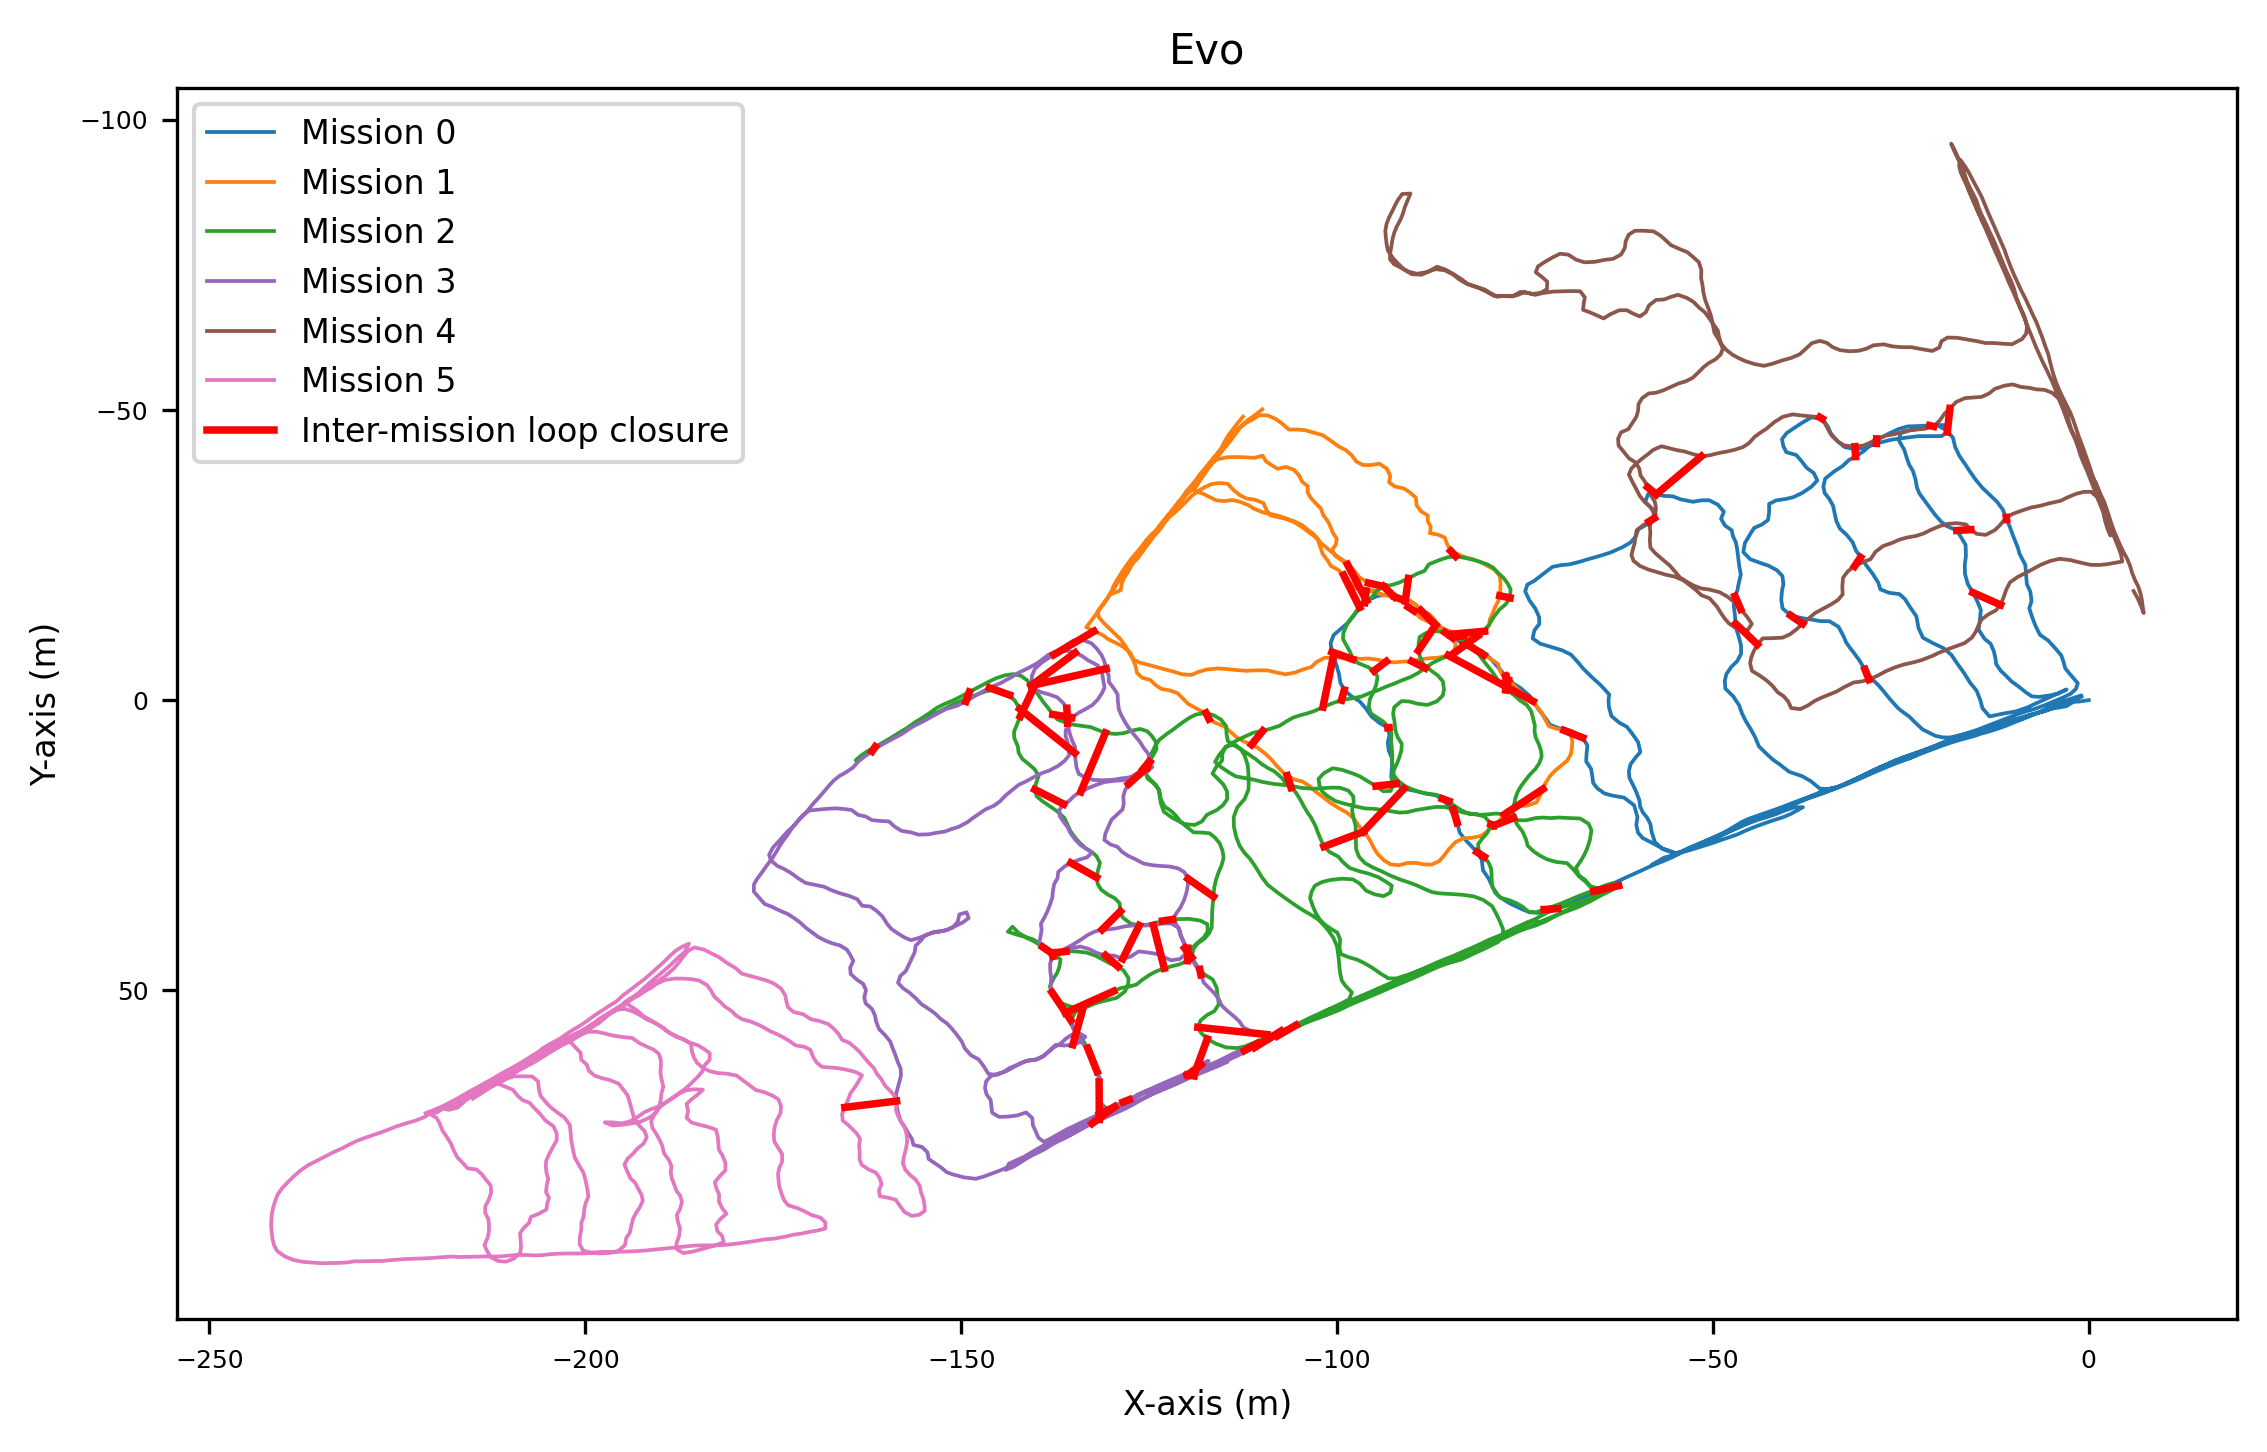
\includegraphics[width=\columnwidth]{pics/exp_3_1_multimission_slam_evo.png}
  \caption{Offline multi-mission SLAM (Evo).}
  \label{fig:exp_multi_mission_evo}
\end{figure}
\newline
\textbf{Wytham Woods, \figref{fig:exp_multi_mission_wytham}} \hspace{0.5em}  Wytham Woods were challenging due to the high tree density, foliage, and vegetation present captured with wide field of view Hesai QT64 LiDAR. Despite these challenges, our system successfully identified loop closures between different missions and merged them as shown in \figref{fig:exp_multi_mission_wytham}. During individual mission processing, slight drifts were noted at the beginning and end of each mission. However, through the multi-mission map merging process, the system successfully corrected these drifts occurring in overlapping areas. Nevertheless, minor drifts still persisted at the edges of the map. 
\begin{figure}[htbp]
  \ContinuedFloat
  \centering
  \includegraphics[width=\columnwidth]{pics/exp_3_offline_wytham_pcd1.png}
  % \caption{Wytam Woods: Offline multi-mission SLAM pointclouds}
  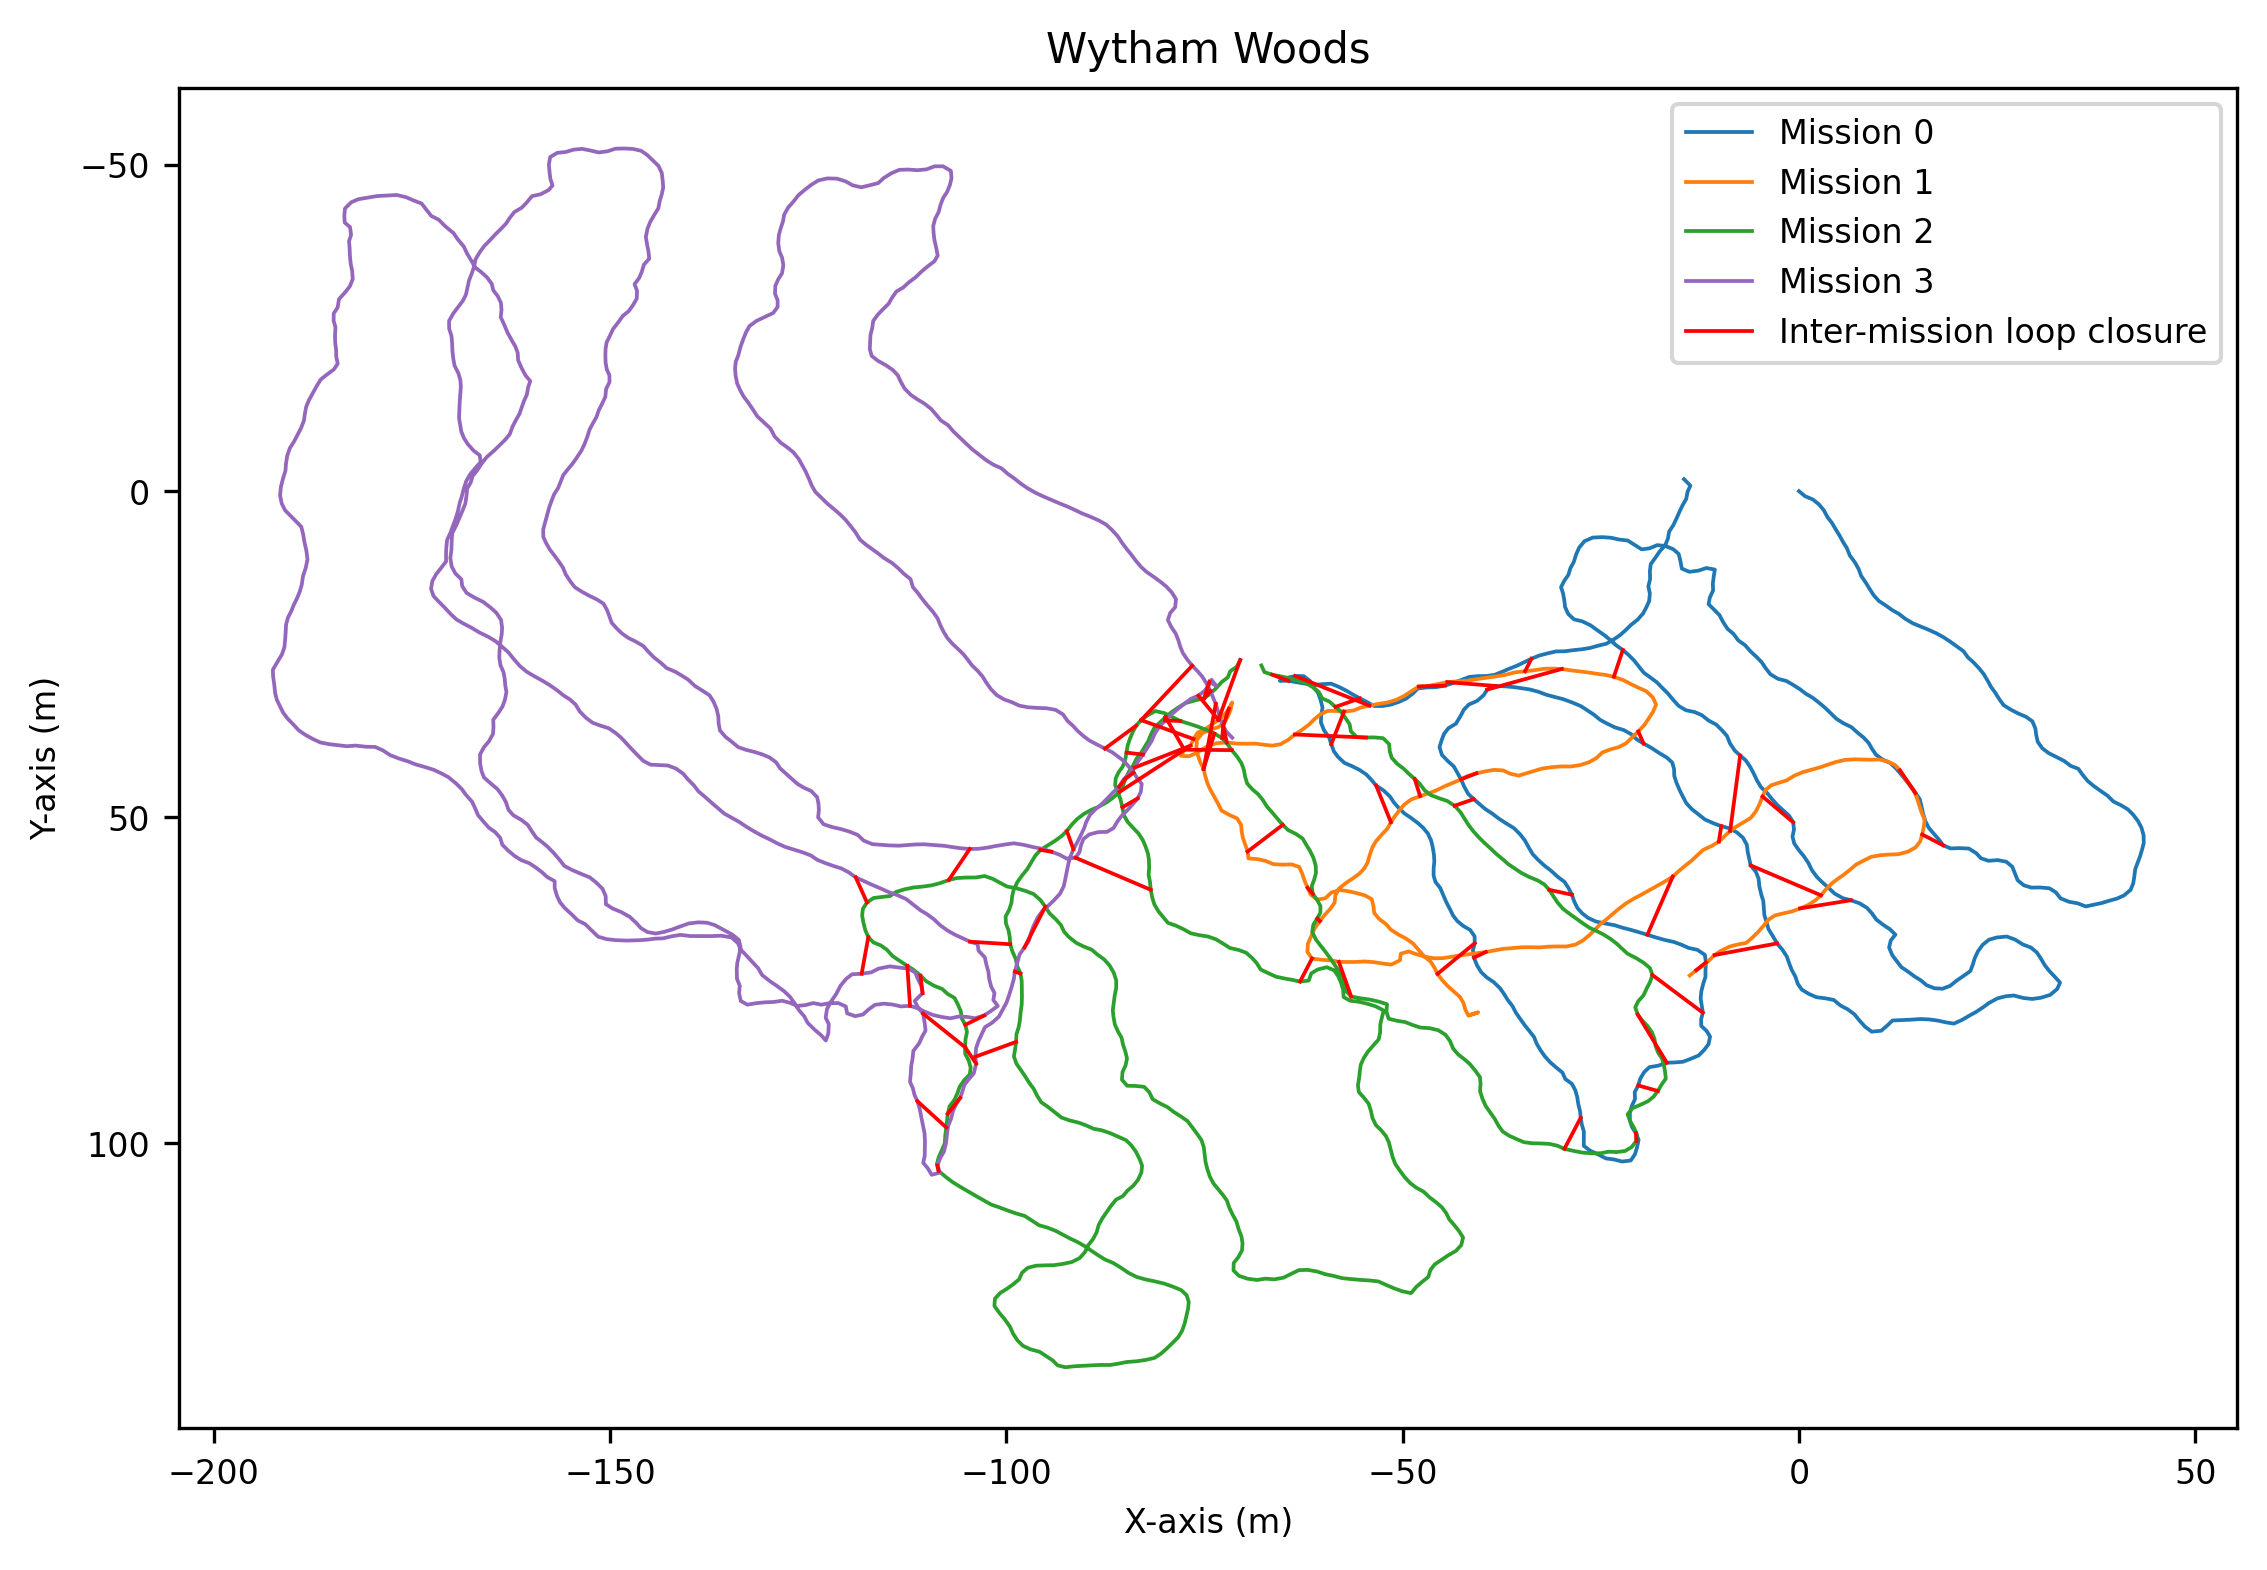
\includegraphics[width=\columnwidth]{pics/exp_3_1_multimission_slam_wytham.png}
  \caption{Wytham Woods: Offline multi-mission SLAM Loop Closures.}
  \label{fig:exp_multi_mission_wytham}
\end{figure}
\newline
\textbf{Forest of Dean, \figref{fig:exp_multi_mission_dean}}\hspace{0.5em} Forest of Dean is less dense forest and 3 missions were merged easily. We observed that there were more frequent \emph{intermission} loop closures in the Forest of Dean compared to Wytham in overlapping areas. 
\begin{figure}[htbp]
  \ContinuedFloat
  \centering
  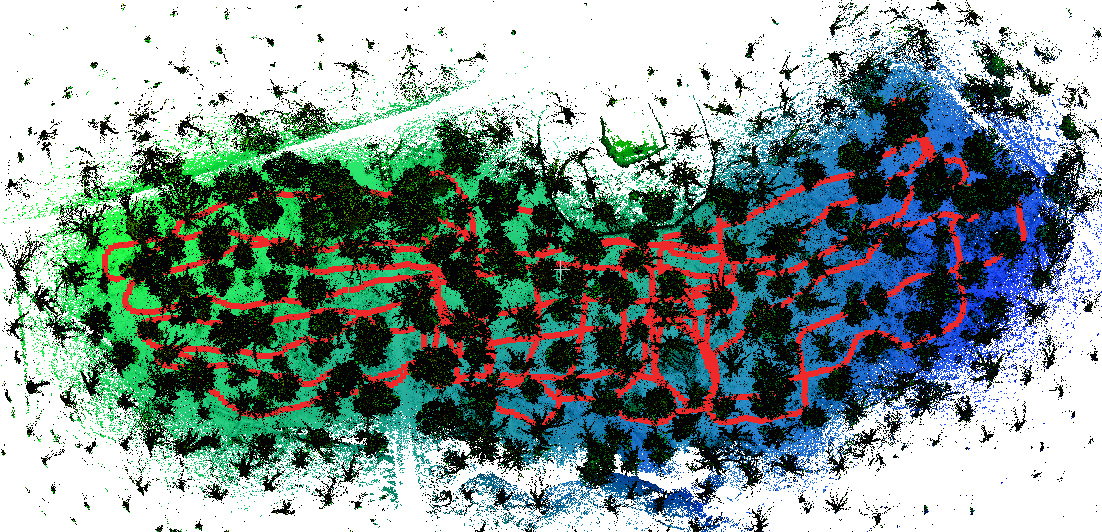
\includegraphics[width=\columnwidth]{pics/exp_3_offline_Dean_pcd3.png}
  % \caption{Forest of Dean: Offline multi-mission SLAM pointclouds}
  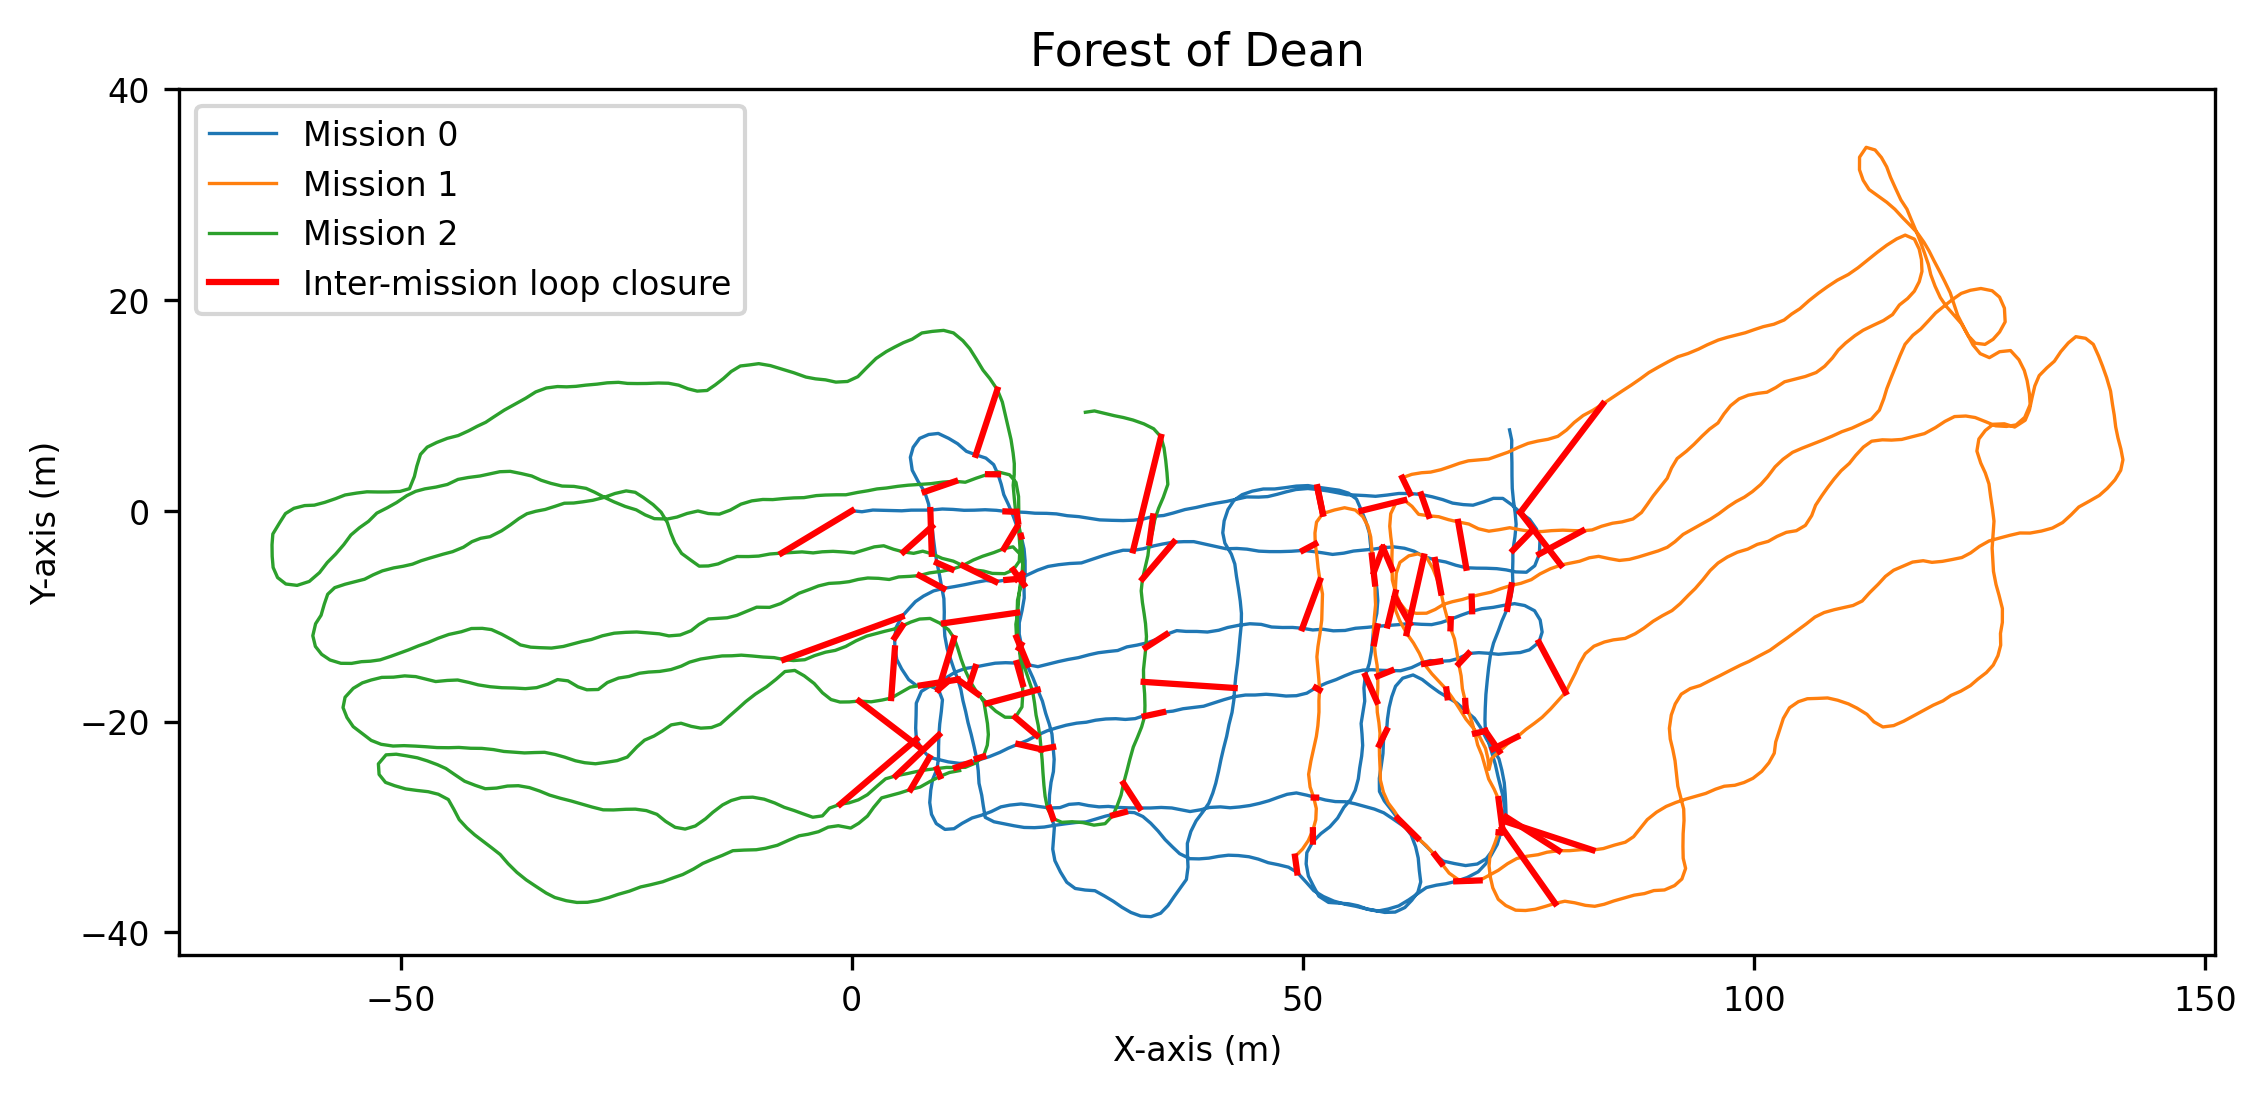
\includegraphics[width=\columnwidth]{pics/exp_3_1_multimission_slam_dean.png}
  \caption{Forest of Dean: Offline multi-mission SLAM Loop Closures.}
  \label{fig:exp_multi_mission_dean}
\end{figure}


Overall, our experiments showed potential for efficient large-scale mapping, as we did not require to start at the open access roads nor following exactly the same paths to achieve loop closures between inter-missions. We also built the map incrementally, one section at a time, hence overlapping areas could only be guaranteed for subsequent missions.

% \tabref{tab:exp_offline_distance_table} provides summary statistics of the distribution of loop closures at different distance ranges. Our multi-stage verification pipeline effectively filters out unreliable loop candidates, with approximately 90\% of successful candidates found within 10\,m of each other. Notably, experiments conducted in Wytham Woods and the Forest of Dean highlight that our system can identify loop closures within the forests, eliminating the need to precisely retrace previously mapped areas to achieve loop closures. This underscores the versatility and robustness of our approach in real-world forest mapping scenarios.

%MF: I removed these comments. I dont think they were adding
%, and facilitates loop-closures with much smaller overlapping areas between inter-missions
%Also, most of them occurred at the start and end of each missions. 
\begin{figure}[t]
  \centering
  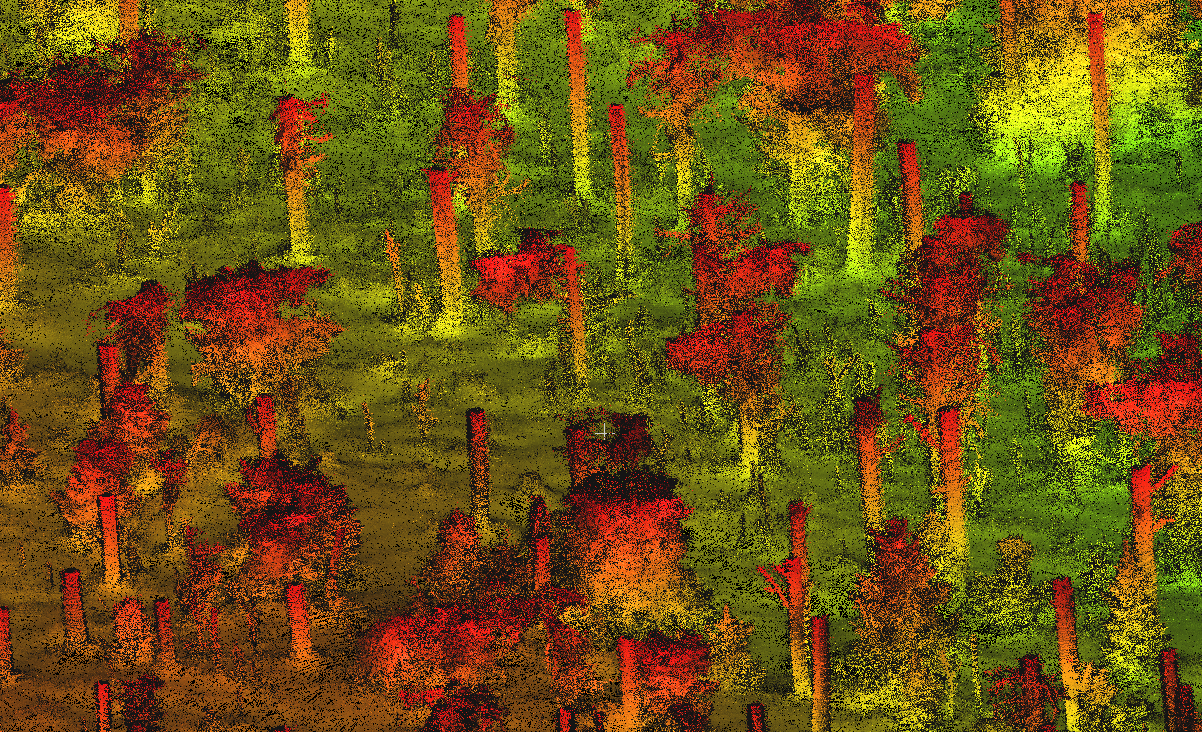
\includegraphics[width=0.9\columnwidth]{pics/exp_3_offline_pointclouds_trunk.png}\label{fig:truk of trees}
  \caption{A region of Evo merged forest map point clouds coloured by height. I cropped canopies to check trunks of trees. Trunks are very distinct showing no evidence of drift occured.}
  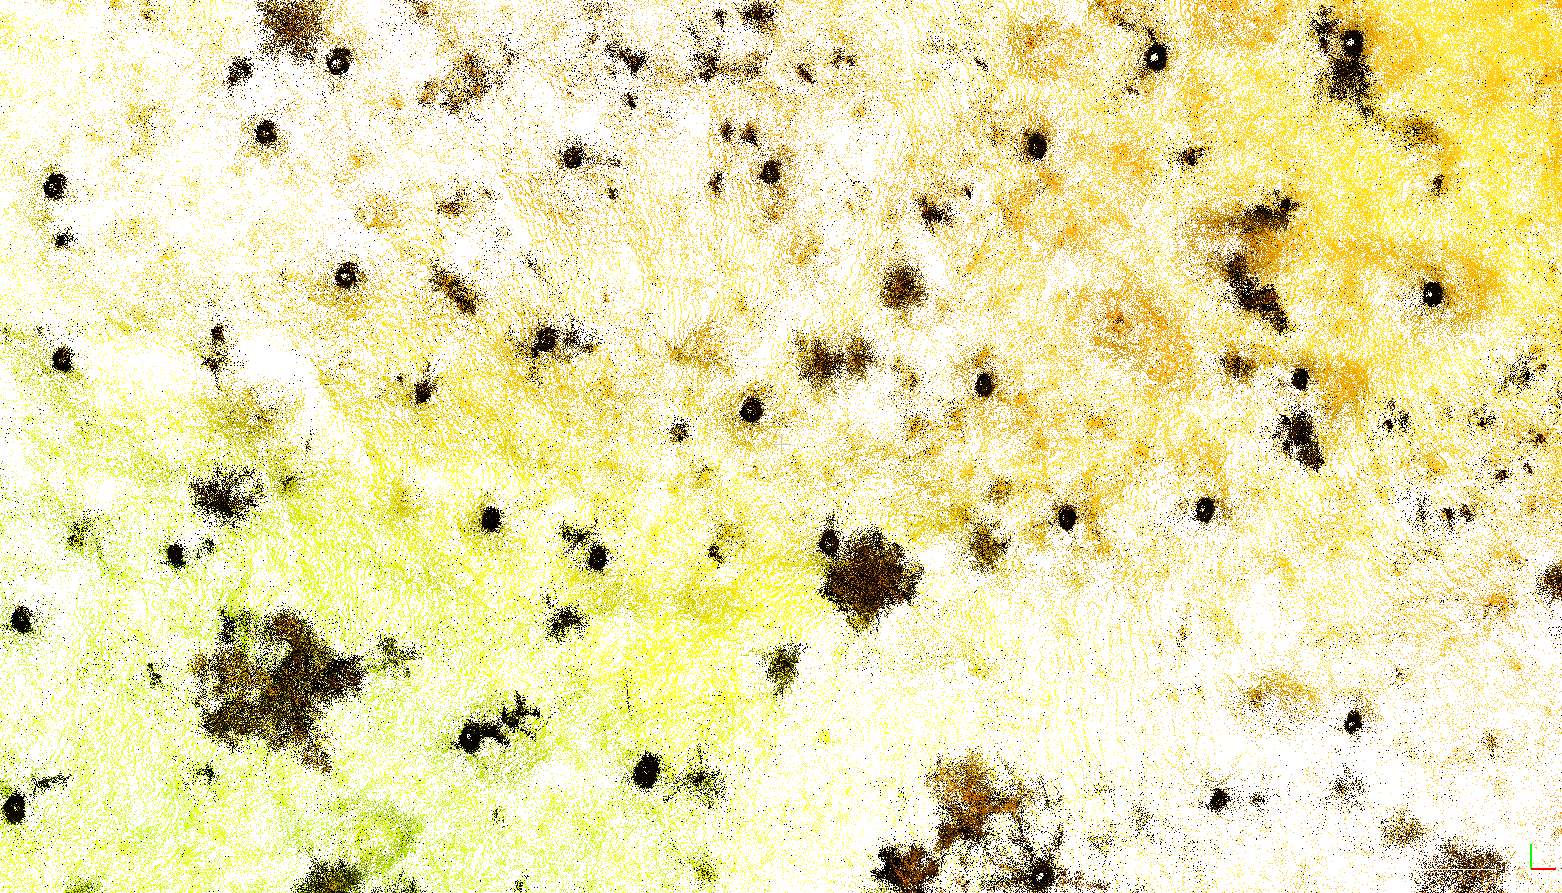
\includegraphics[width=0.9\columnwidth]{pics/exp_3_offline_pointclouds_trunk_BV3.png}\label{fig:trunk of trees BV}
  \caption{Trunks of trees from Berd's eye view. We observed circular shapes for tree trunks clearly seen in the point clouds, indicating the map scanned in different viewpoints were registered correctly.}
\end{figure}


% \begin{figure*}[htbp]
%   \centering
%   \includegraphics[width=0.90\columnwidth]{pics/exp_3_1_multimission_slam_wytham.png}
%   \includegraphics[width=0.90\columnwidth]{pics/exp_3_1_multimission_slam_evo.png}
%   \includegraphics[width=0.90\columnwidth]{pics/exp_3_1_multimission_slam_dean.png}
%   \caption{Offline multi-mission SLAM. Left: Wytham - a densely wooded area with uneven terrain, including hills. Center: Evo - featuring a LiDAR setup on an incline, with loop closures occurring primarily when viewpoints are closely aligned. Right: Forest of Dean - flatter terrain compared to Wytham, with a sparser plantation, allowing for loop closures to be captured at greater distances. }
%   \label{fig:exp_multi_mission}
% \end{figure*}


% \begin{table}[htbp]
%   \centering
%   \small
%   \begin{tabular}{p{2cm}cccc}
%       \toprule
%       \multicolumn{1}{l}{loop closures} & \multicolumn{3}{c}{Dataset} \\
%       \multicolumn{1}{l}{distance range (m)} & Wytham & Evo & Forest of Dean \\
%       \midrule
%       0-5\,m &41 / 53\%  &83 / 78\%  &73 / 78\% \\
%       \midrule
%       5-10\,m &29 / 37\%  &19 / 18\% &15 / 16\%\\
%       \midrule
%       10-15\,m &8 / 10\%  &4 / 4\%   &6 / 6\% \\
%       \midrule
%       Total  & 78 / 100\%  & 106 / 100\%  & 94 / 100\% \\
%       \bottomrule
%   \end{tabular}
%   \caption{Offline Multi-mission map merging results corresponding to \figref{fig:exp_multi_mission}: Number and percentage of final inter-mission loop closures detected by distance between matched poses.}
%   %Setting rigorous thresholds on number of descriptors, SGV, pairwise consistency check and ICP registration allows robust loop-closure pairs to be found, with any loop-candidates more than 15m away rejected  
%   \label{tab:exp_offline_distance_table}
% \end{table}




% Fourth experiment: Relocalization 
\section{Relocalization} 
\label{sec:exp_relocalization}
% What is this experiment about?
This experiment showcases a relocalization demonstration in a dense forest using our approach. In this scenario, our system demonstrates the ability to continuously track the position within a prior SLAM map once an initial loop closure is established.
% What are some particular characteristic?
%Unlike multi-mission, since prior map poses are fixed as ground truth,  we no longer jointly optimize poses.
%Instead, we found that precision of 6DOF localization itself affects pairwise consistency of loop-closures.
%Therefore, we limit the pairwise consistency threshold at few centimeter level. This enables continuous relocalization only within centimeter level of error, while reducing recall. 
Figure \ref{fig:relocalization} presents an illustrative example of this demonstration, where the quadruped robot shown in \figref{fig:relocalization} is localized with respect to a prior SLAM map generated using a backpack LiDAR system. This capability enables the real-time rendering of a virtual forest map overlaid with associated data, such as Diameter at Breast Height (DBH) and species information, onto the camera images. Such feedback is highly beneficial for tasks such as taking forest inventories by foresters or enabling autonomous harvesting.
\begin{figure}[htbp]
  \centering
  \includegraphics[width=0.99\linewidth]{pics/exp_4_relocalization_demo.png}
  \caption{Demonstration of relocalization capability. LiDAR (illustrated by large marker) is relocalized in a prior map. We render a virtual view of the forest digital map synchronized with images from our camera (right). Red arrow shows a successful localization at that pose.}
  \label{fig:relocalization}
\end{figure}

\subsection*{Pairwise Cycle Consistency Check}
We can check how effective pairwise consistency check is in relocalization. We can see that the number of loop-closures detected by pairwise consistency check is reduced as the distance between the loop-candidates increases. This is because the precision of 6DOF localization itself affects pairwise consistency of loop-closures. Therefore, we limit the pairwise consistency threshold at few centimeter level. This enables continuous relocalization only within centimeter level of error, while reducing recall. 

\subsection*{Time / Distance to relocalize}
We checked how long it takes to relocalize and how far the robot can move before relocalization fails. We found that the system can relocalize within 1 second and 1 meter of distance. This is because we limit the pairwise consistency threshold at few centimeter level. This enables continuous relocalization only within centimeter level of error, while reducing recall.

%%%%%%%%%%%%%%%%%%%%%%%%
\section{Discussion \& Ablation Studies}


\subsection*{Study of ICP inlier-based check}
\label{sec:exp_icp_ablation}

Our final experiment investigates the ICP inlier-based check on loop closure integration within the final pose graph optimization process. This analysis is crucial for ensuring that incorrect loop closures are not introduced into the optimized pose graph.
\figref{fig:icp_inliers} illustrates the corrections (on top of the initial transformation prior) as estimated by the ICP registration at various distances. Additionally, the figure color-codes the points based on the number of inlier points obtained during the registration process, with blue indicating a large number of inliers and red indicating a smaller number.
Our observation suggests that loop closures occurring beyond 10\,m, which propose a substantial transformation correction often have fewer inlier ICP points and are thus less reliable.
Based on this analysis, we establish an inlier threshold to ensure that corrections are limited to ICP corrections of less than 1 meter (shown in dotted red line). This threshold further reduces the number of incorrect loop closures from being integrated into the pose graph.
\begin{figure}[t]
  \centering
  \includegraphics[width=0.99\linewidth]{pics/exp_4_ablation_icp_inliers_4cm}
  \caption{Analysis of final ICP registration check. X-axis shows the distribution of loop-candidates by distance after ICP.
  Y-axis shows ICP correction error w.r.t. the coarse-registration from RANSAC. Color indicates the number of ICP inliers,  30 iterations and RMSE= 0.01m, where clouds are cropped 50 by 50m, then downsampled to 20k points.}
  \label{fig:icp_inliers}
\end{figure}



% What is the interpretation of the figure?
% Alongside \figref{fig:exp_2_2_loop_closure_histograms}, further analysis has been done how robust the loop-candidates are. 
% \figref{fig:ablation_icp_inliers} shows that under 10m distance, ICP inliers are high as over 4k points, and correction error is below 1m. However, the distribution of loop-candidates start to diverge significantly after 10m: correction error no longer bounds to 1m and the number of inliers are much less than 4k points. 
% Setting a low ICP inlier threshold will provide far distance loop-closures, but there is a chance of getting False Positives.
\subsection*{Computation Analysis}
top-1 to top-5 candidates Run time analysis.

\subsection*{Parameters}
There are several important parameters that should be tuned in our system for ddifferent LiDAR setups and different forest environments. \\
\textbf{Voxel Size}\hspace{0.5em} During preprocessing step it is necessary to voxelize input point clouds for discritize representation using \emph{MinkosckiEngine, SparseTorch}. This voxel size is known to be critical for the performance of the model descriptors. Since both Logg3dNet and EgoNN are trained on WildPlace dataset, which is different from our dataset in terms of density and range of LiDAR point clouds, We empirically determined the optimal voxel size between \SIrange{0.1}{1.0}{\meter} through direct experimentation on our dataset. Tab.~\ref{tab:voxel_size} shows that optimal voxel sizes are \SI{0.1}{\meter} and \SI{0.6}{\meter} for Logg3dNet on Evo dataset. Since the difference is not significant, we decided to use voxel size of \SI{0.6}{\meter} considering computational efficiency.\\

\begin{table}[htbp]
  \centering
  \begin{tabular}{p{2cm} *{6}{c}}
      \toprule
      \multicolumn{1}{l}{Testing} & \multicolumn{6}{c}{Voxel size (cm)} \\
      \cmidrule{2-7}
      \multicolumn{1}{l}{Datasets} & 10 & 20 & 40 & 60 & 80 & 100 \\
      \midrule
      Evo-12 &\textbf{0.89} &0.79 &0.77 &\textbf{0.86} &0.79 &0.78 \\
      \addlinespace % Add space between rows
      Evo-16 & \textbf{0.74} & 0.66 & 0.66 & \textbf{0.66} & 0.64 & 0.63 \\
      \addlinespace % Add space between rows
      Evo-18  &0.71 & 0.75 & \textbf{0.75} & \textbf{0.76} & 0.73 & 0.71 \\
      \bottomrule
  \end{tabular}

  \caption{$F{1}_{max}$ score of Logg3dNet with different voxel sizes on Evo dataset. Bold numbers indicate the best and second best $F{1}_{max}$ score.}
  \label{tab:voxel_size}
\end{table}

  
\textbf{ICP inlier threshold} \hspace{0.5em} ICP inliers threshold is the least number of inliers to consider the ICP registration as successful at final verification step. As discussin in \secref{sec:icp_inliers}, the threshold is fine tuned to $sim$ 3k-5k points depending on the LiDAR setup and forest environments. 

  
\textbf{Failure cases}


- Descriptor distance 


- LIOSAM Odometry system 



% \include{chapters/ch6-wvn}
% \include{chapters/ch7-autonomous-inventory}
\chapter{Conclusion}
\label{chap:conclusion}

In this thesis, we conducted extensive testing of LiDAR place recognition systems in dense forest environments. We presented a place recognition and verification system that leverages three stages of loop-candidate verification: at the global descriptor-level, local feature-level, and fine point cloud level. These place recognition modules were seamlessly integrated into a pose graph SLAM system and evaluated across three distinct scenarios: online SLAM, offline multi-mission SLAM, and relocalization. Our experiments provide further insights on the performance of currently available LiDAR-based place recognition methods in dense forests. We also studied three different applications which could take advantage of this 6-DoF localization, opening future applications for forest inventory, inspection, and autonomous tasks. 

In future work, we plan to use this system to function as a standalone \textit{place recognition server}, allowing for easier integration of new LiDAR place recognition methods and to make it available for use by other members of the DRS group. We also plan to deploy the place recognition server in real-time on a Frontier device with an NVidia Jetson GPU board in future field trials. 


% %% APPENDICES %% 
% % Starts lettered appendices, adds a heading in table of contents, and adds a
% %    page that just says "Appendices" to signal the end of your main text.
% \startappendices
% % Add or remove any appendices you'd like here:
% 
\chapter{Other contributions}
\label{app:A}

\hyphenation{de-bayer-ing}

%\section{Software and tutorials}
In addition to the publications that were presented in \secref{sec:thesis-publications}, additional contributions of this thesis include open-source software and tutorials:

\begin{enumerate}[leftmargin=*]
	%\item \texttt{field\_local\_planner}: Implementation of the local planner presented in \textcite{Mattamala2022}:\\ \url{https://github.com/ori-drs/field_local_planner}
	%
	%\item \texttt{grid\_map\_filters\_drs}: Package for local map procesing, including implementations of \gls{sdf} and \gls{gdf}:\\
	%\url{https://github.com/ori-drs/grid_map_filters_drs}
	%
	\item \texttt{raw\_image\_pipeline}: An open-source raw image processing pipeline for debayering, white balancing, and undistortion:\\
	\url{https://github.com/leggedrobotics/raw_image_pipeline}
	%
	\item \texttt{digiforest\_analysis} and \texttt{digiforest\_analysis\_ros}: A Python package and ROS wrapper that implement the forest analysis pipeline presented in \chapref{chap:autonomous-forest-inventory}:\\
	\url{https://github.com/ori-drs/digiforest_drs}
	%
	\item \textbf{Tutorial on optimisation-based state estimation}: A comprehensive review of optimisation on manifolds and uncertainty propagation on Lie groups.
	\begin{itemize}
		\item Linear and non-linear state estimation:\\
		\url{https://gtsam.org/2021/02/23/uncertainties-part1.html} 
		%
		\item Frames frames, manifolds, and Lie groups:\\
		\url{https://gtsam.org/2021/02/23/uncertainties-part2.html} 
		%
		\item Uncertainty propagation on Lie groups:\\
		\url{https://gtsam.org/2021/02/23/uncertainties-part3.html} 
	\end{itemize}
\end{enumerate}
% 
\chapter{Autonomous Legged Forester Robot: Additional Plots}
\label{app:B}

% \section{Reconstructions}
% \begin{figure}[!htb]
% 	\includegraphics[width=\textwidth]{figures/legged_forester/m1-map-labeled.png}
% 	\caption{Map and trajectory obtained in Mission 1, executed on site B. This was the first large-scale deployment.}
% 	\label{fig:alf-m1-map}
% \end{figure}

% \begin{figure}[!htb]
% 	\includegraphics[width=\textwidth]{figures/legged_forester/m2-map-labeled.png}
% 	\caption{Map and trajectory obtained in Mission 2, executed on site B. This mission was fully autonomous.}
% 	\label{fig:alf-m2-map}
%   \end{figure}
  
% \begin{figure}[!htb]
% 	\includegraphics[width=\textwidth]{figures/legged_forester/m3-map-labeled.png}
% 	\caption{Map and trajectory obtained in Mission 3, executed on site B. This mission was interrupted, due to the robot getting stuck on a damp area.}
% 	\label{fig:alf-m3-map}
% \end{figure}
  
% \begin{figure}[!htb]
% 	\includegraphics[width=\textwidth]{figures/legged_forester/m4-map-labeled.png}
% 	\caption{Map and trajectory obtained in Mission 4, executed on site C.}
% 	\label{fig:alf-m4-map}
% \end{figure}
  
% \begin{figure}[!htb]
% 	\includegraphics[width=\textwidth]{figures/legged_forester/m5-map-labeled.png}
% 	\caption{Map and trajectory obtained in Mission 5, executed on site A. State estimation errors caused a significant drift that impeded the robot from returning to the operator's location.}
% 	\label{fig:alf-m5-map}
% \end{figure}

\section{Speed Profiles}
We report detailed speed profiles to provide further details on the performance of the autonomous legged forester robot on the five missions described in \tabref{tab:alf-campaign}. The speed profiles show the commanded velocity (from the local planner), the measured velocity (from the odometry system), as well as the safety interventions (done by the safety operator).

\begin{figure}[ht]
	\centering
	\includegraphics[width=\textwidth]{figures/legged_forester/mission_velocity_m1.pdf}
	\caption{Speed profile and interventions in mission M1.}
	\label{fig:alf-m1-speed}
\end{figure}

\begin{figure}[ht]
	\centering
	\includegraphics[width=\textwidth]{figures/legged_forester/mission_velocity_m2.pdf}
	\caption{Speed profile and interventions in mission M2.}
	\label{fig:alf-m2-speed}
\end{figure}

\begin{figure}[ht]
	\centering
	\includegraphics[width=\textwidth]{figures/legged_forester/mission_velocity_m3.pdf}
	\caption{Speed profile and interventions in mission M3.}
	\label{fig:alf-m3-speed}
\end{figure}

\begin{figure}[ht]
	\centering
	\includegraphics[width=\textwidth]{figures/legged_forester/mission_velocity_m4.pdf}
	\caption{Speed profile and interventions in mission M4.}
	\label{fig:alf-m4-speed}
\end{figure}


\begin{figure}[!ht]
	\centering
	\includegraphics[width=\textwidth]{figures/legged_forester/mission_velocity_m5.pdf}
	\caption{Speed profile and interventions in mission M5.}
	\label{fig:alf-m5-speed}
\end{figure}



%%%%% REFERENCES

%IEEE
%Can I Reuse My Published Article in My Thesis?
%
%You may reuse your published article in your thesis or dissertation without requesting permission, provided that you fulfill the following requirements depending on which aspects of the article you wish to reuse.
%
%Text excerpts: Provide the full citation of the original published article followed by the IEEE copyright line: © 20XX IEEE. If you are reusing a substantial portion of your article and you are not the senior author, obtain the senior author’s approval before reusing the text.
%Graphics and tables: The IEEE copyright line (© 20XX IEEE) should appear with each reprinted graphic and table.
%Full text article: Include the following copyright notice in the references: “© 20XX IEEE. Reprinted, with permission, from [full citation of original published article].”
%
%When posting your thesis on your university website, include the following message:
%
%“In reference to IEEE copyrighted material which is used with permission in this thesis, the IEEE does not endorse any of [name of university or educational entity]’s products or services. Internal or personal use of this material is permitted. If interested in reprinting/republishing IEEE copyrighted material for advertising or promotional purposes or for creating new collective works for resale or redistribution, please go to http://www.ieee.org/publications_standards/publications/rights/rights_link.html to learn how to obtain a License from RightsLink. If applicable, University Microfilms and/or ProQuest Library, or the Archives of Canada may supply single copies of the dissertation.”
%
%Only the accepted version of your article, not the final published version, may be posted online in your thesis.

% \setlength{\baselineskip}{0pt} % JEM: Single-space References


\printbibheading
% \printbibliography[type=book,heading=subbibliography,title={References}]
\printbibliography
% {\renewcommand*\MakeUppercase[1]{#1}%
% \printbibliography[heading=bibintoc,title={References}]}


\end{document}
